\chapter{Test Beam Calibration Validation Plots}\label{sec:AppTBCalibValid}

\section{Distributions for Stopping Muons}

\begin{figure}[!ht]
  \begin{subfigure}{\textwidth}
  \centering
    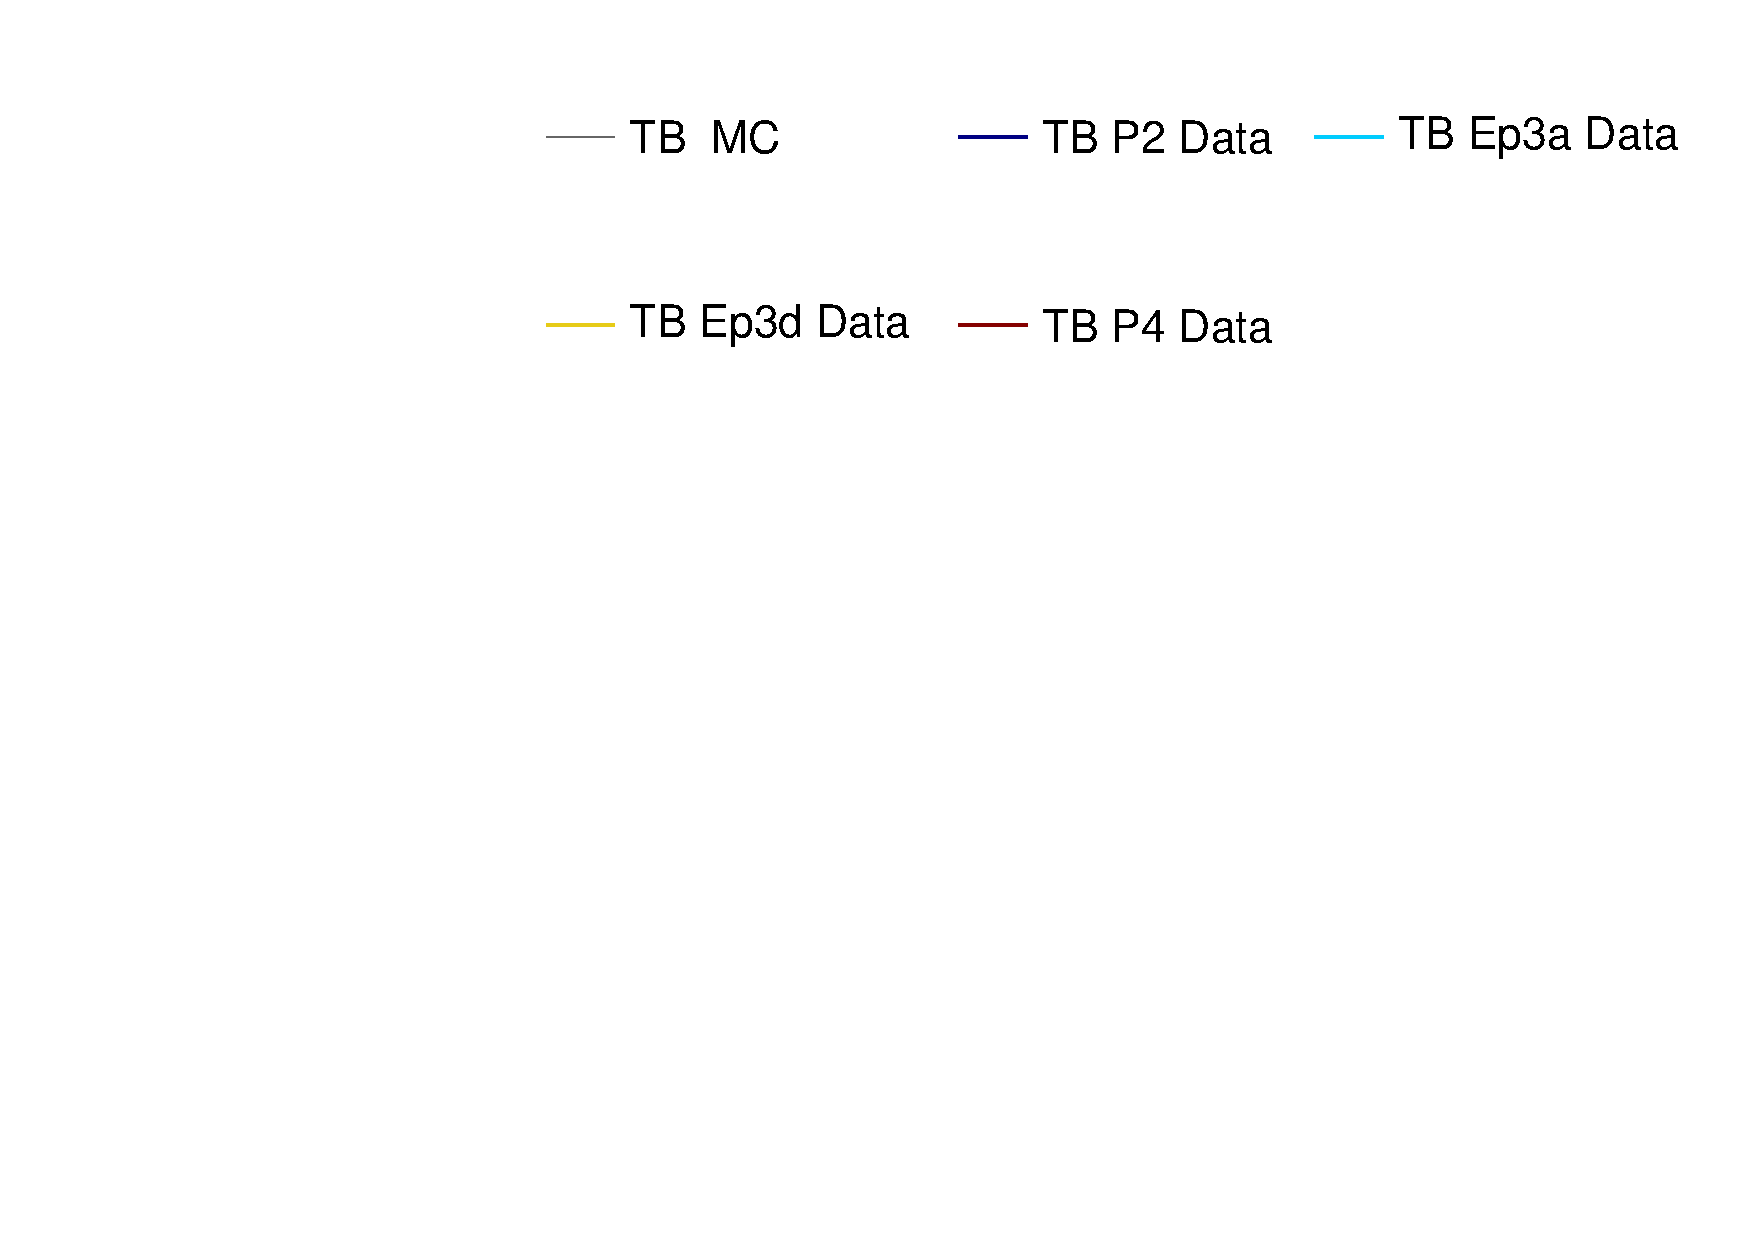
\includegraphics[height=0.2\linewidth]{Plots/Calibana/legend.pdf}
  \end{subfigure}
  \vspace*{2mm}
  
  \begin{subfigure}{0.495\textwidth}
    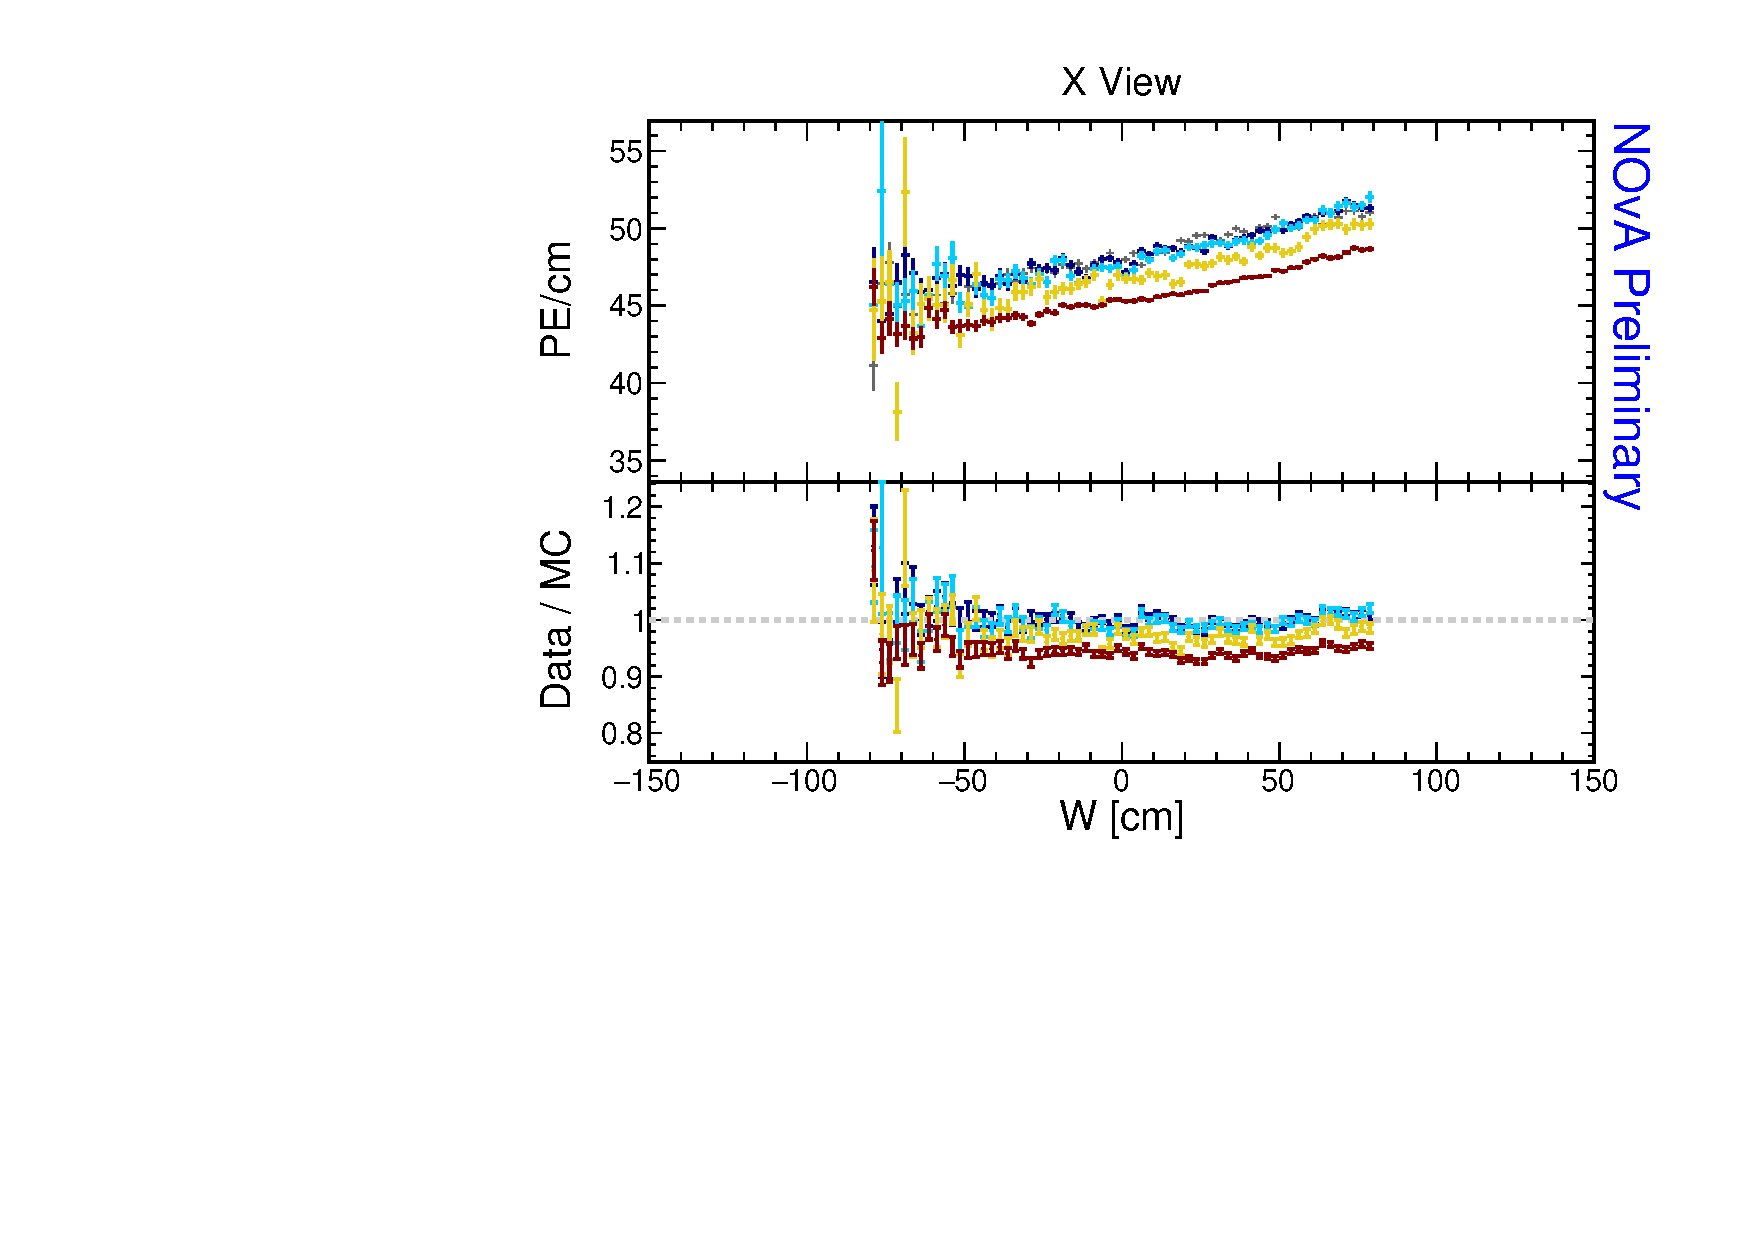
\includegraphics[width=\linewidth]{Plots/Calibana/pecm_w_x.pdf}
  \end{subfigure}
  \begin{subfigure}{0.495\textwidth}
    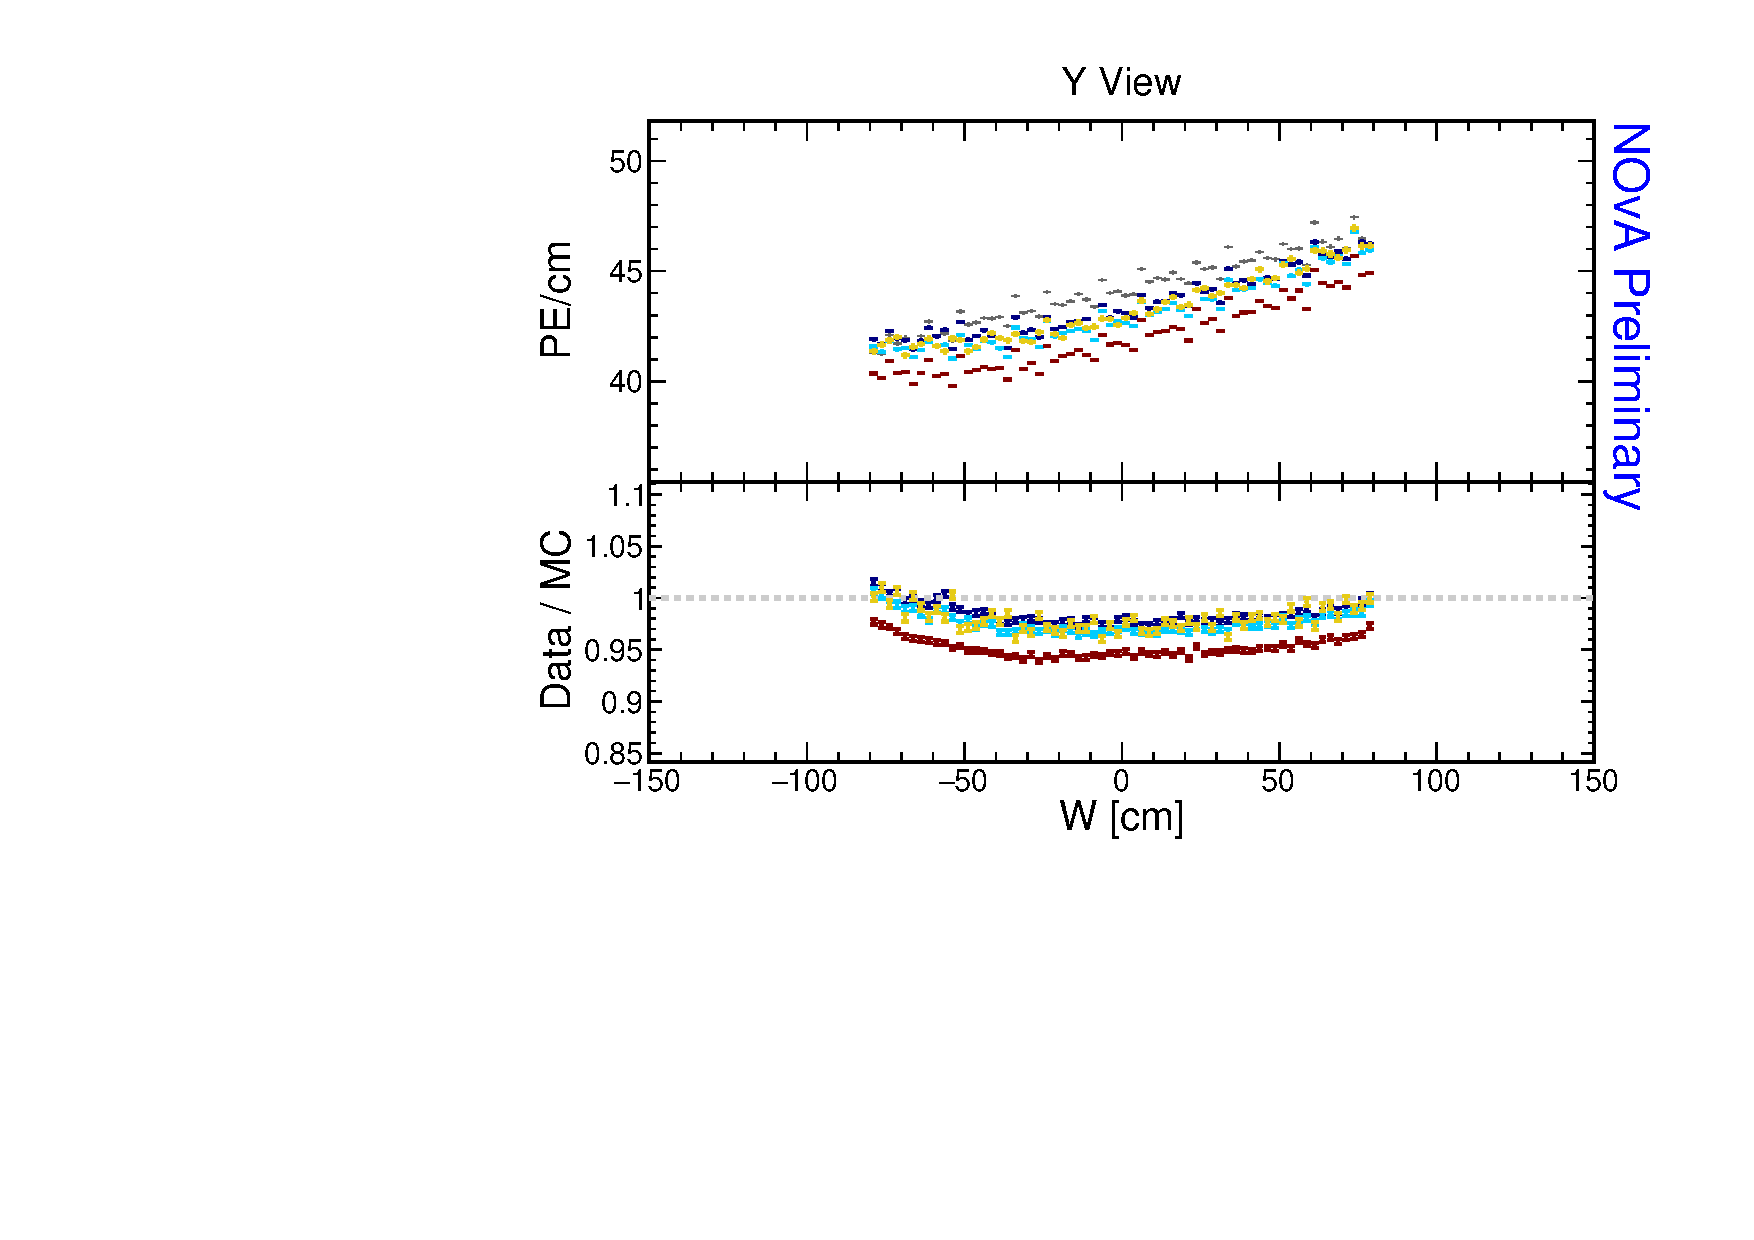
\includegraphics[width=\linewidth]{Plots/Calibana/pecm_w_y.pdf}
  \end{subfigure}
  \begin{subfigure}{0.495\textwidth}
    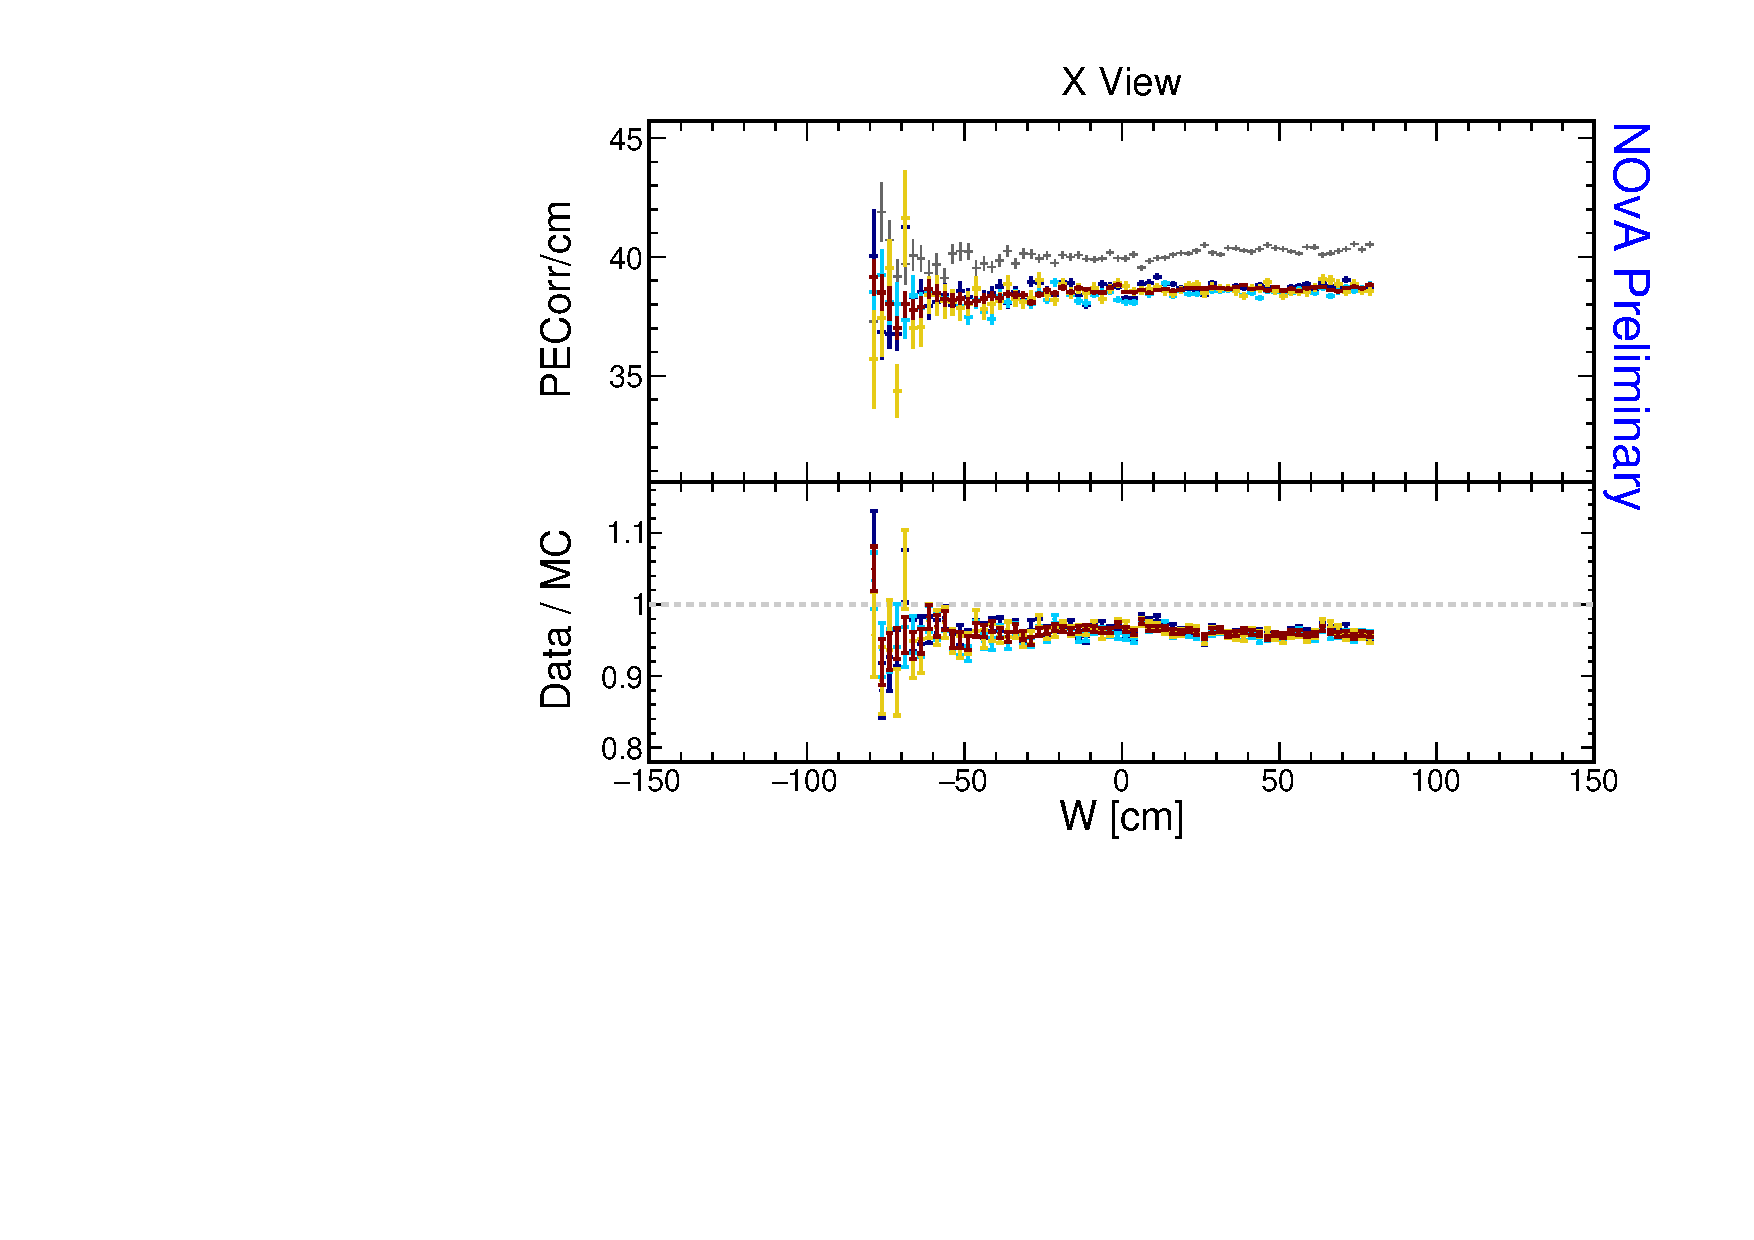
\includegraphics[width=\linewidth]{Plots/Calibana/pecorrcm_w_x.pdf}
  \end{subfigure}
  \begin{subfigure}{0.495\textwidth}
    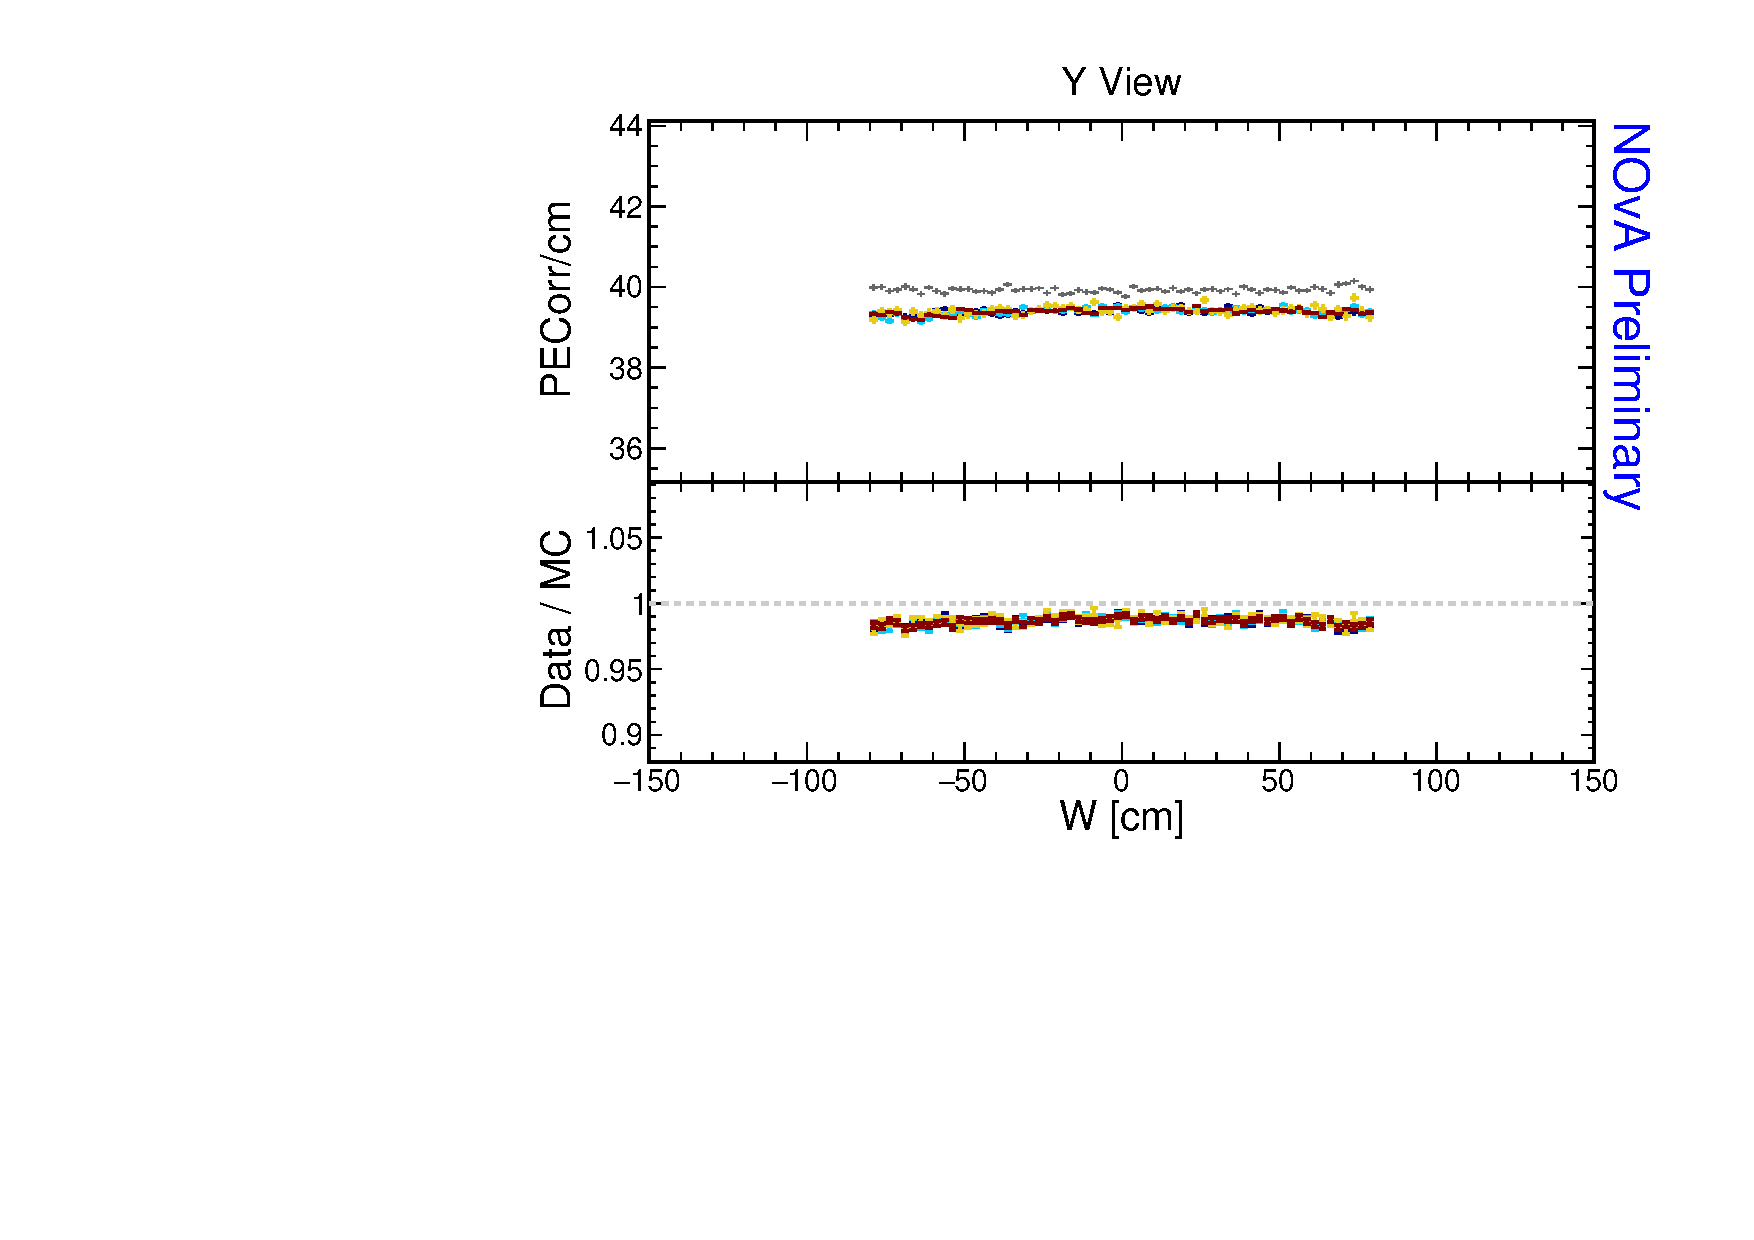
\includegraphics[width=\linewidth]{Plots/Calibana/pecorrcm_w_y.pdf}
  \end{subfigure}
    \begin{subfigure}{0.495\textwidth}
    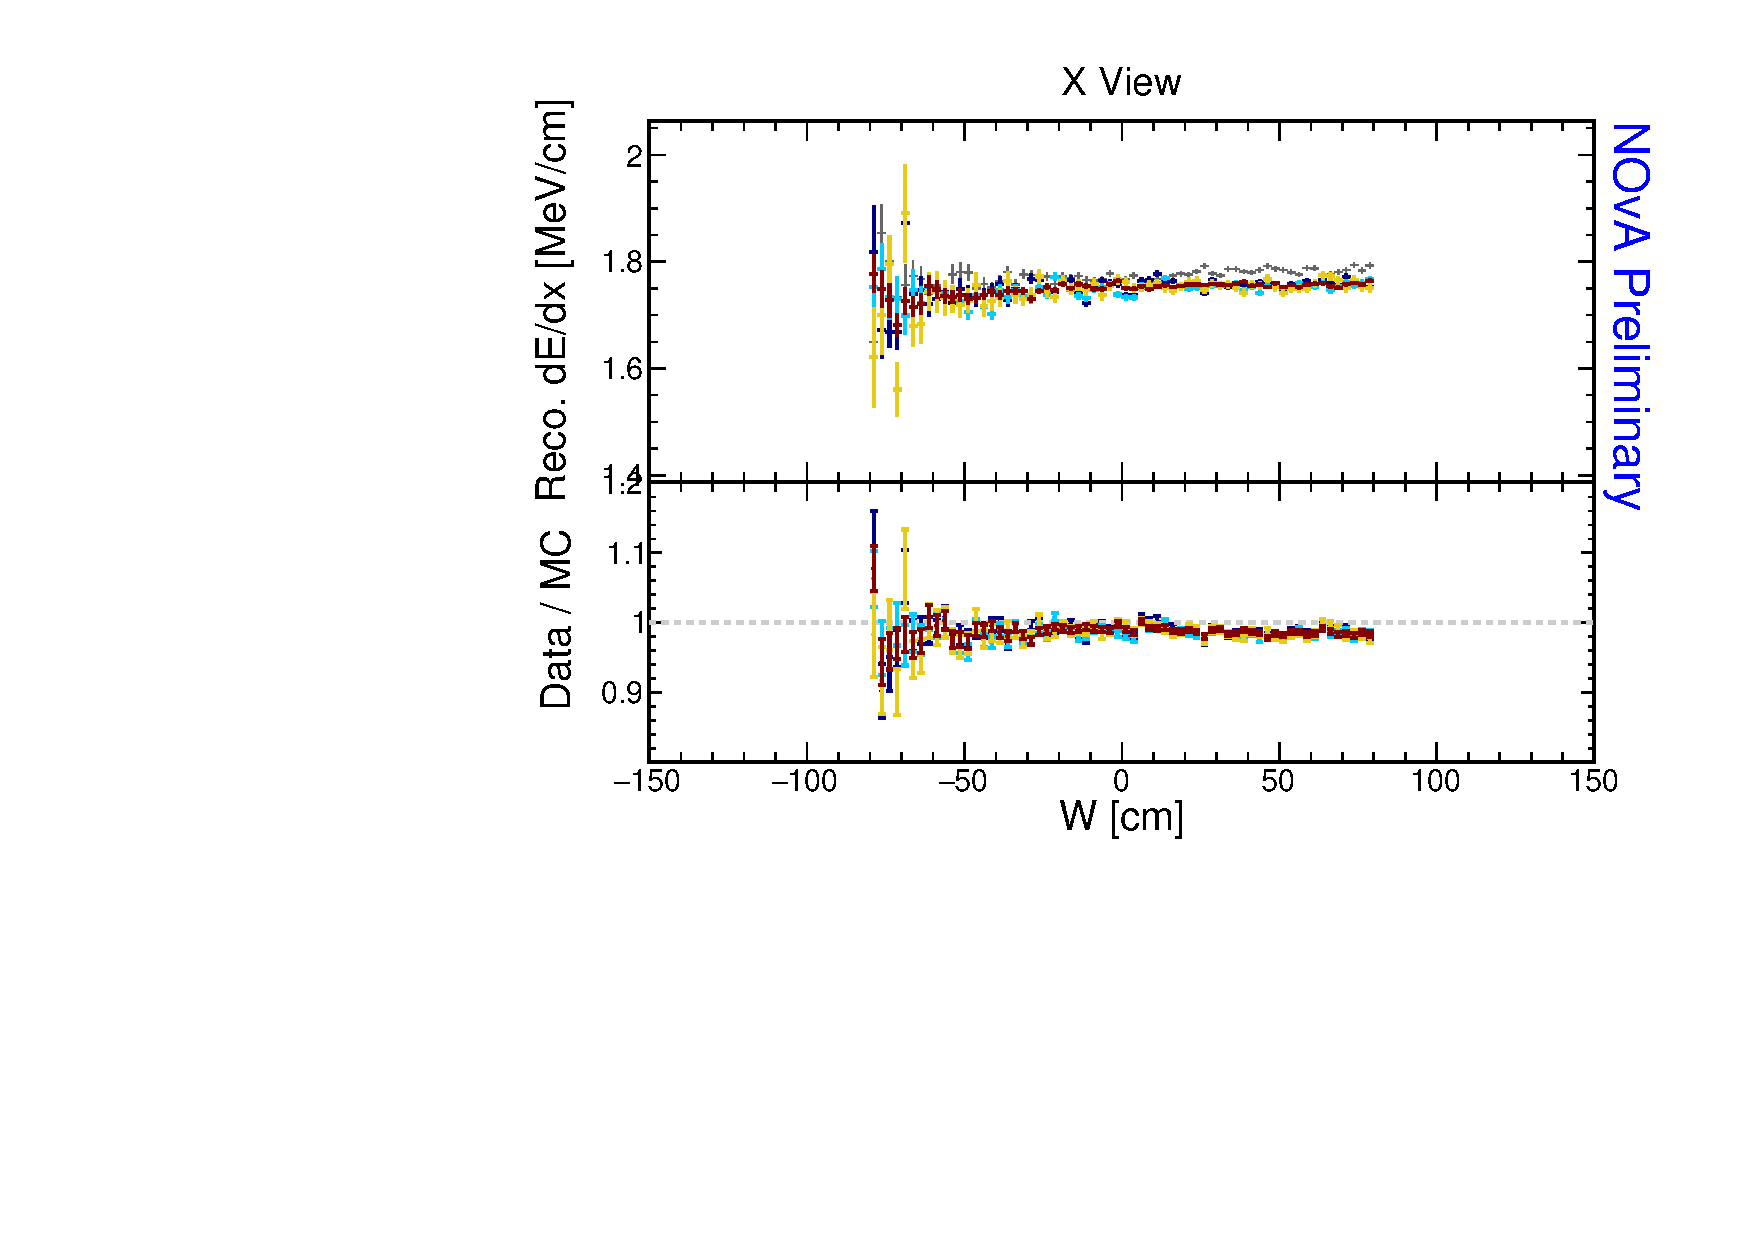
\includegraphics[width=\linewidth]{Plots/Calibana/recomevcm_w_x.pdf}
  \end{subfigure}
  \begin{subfigure}{0.495\textwidth}
    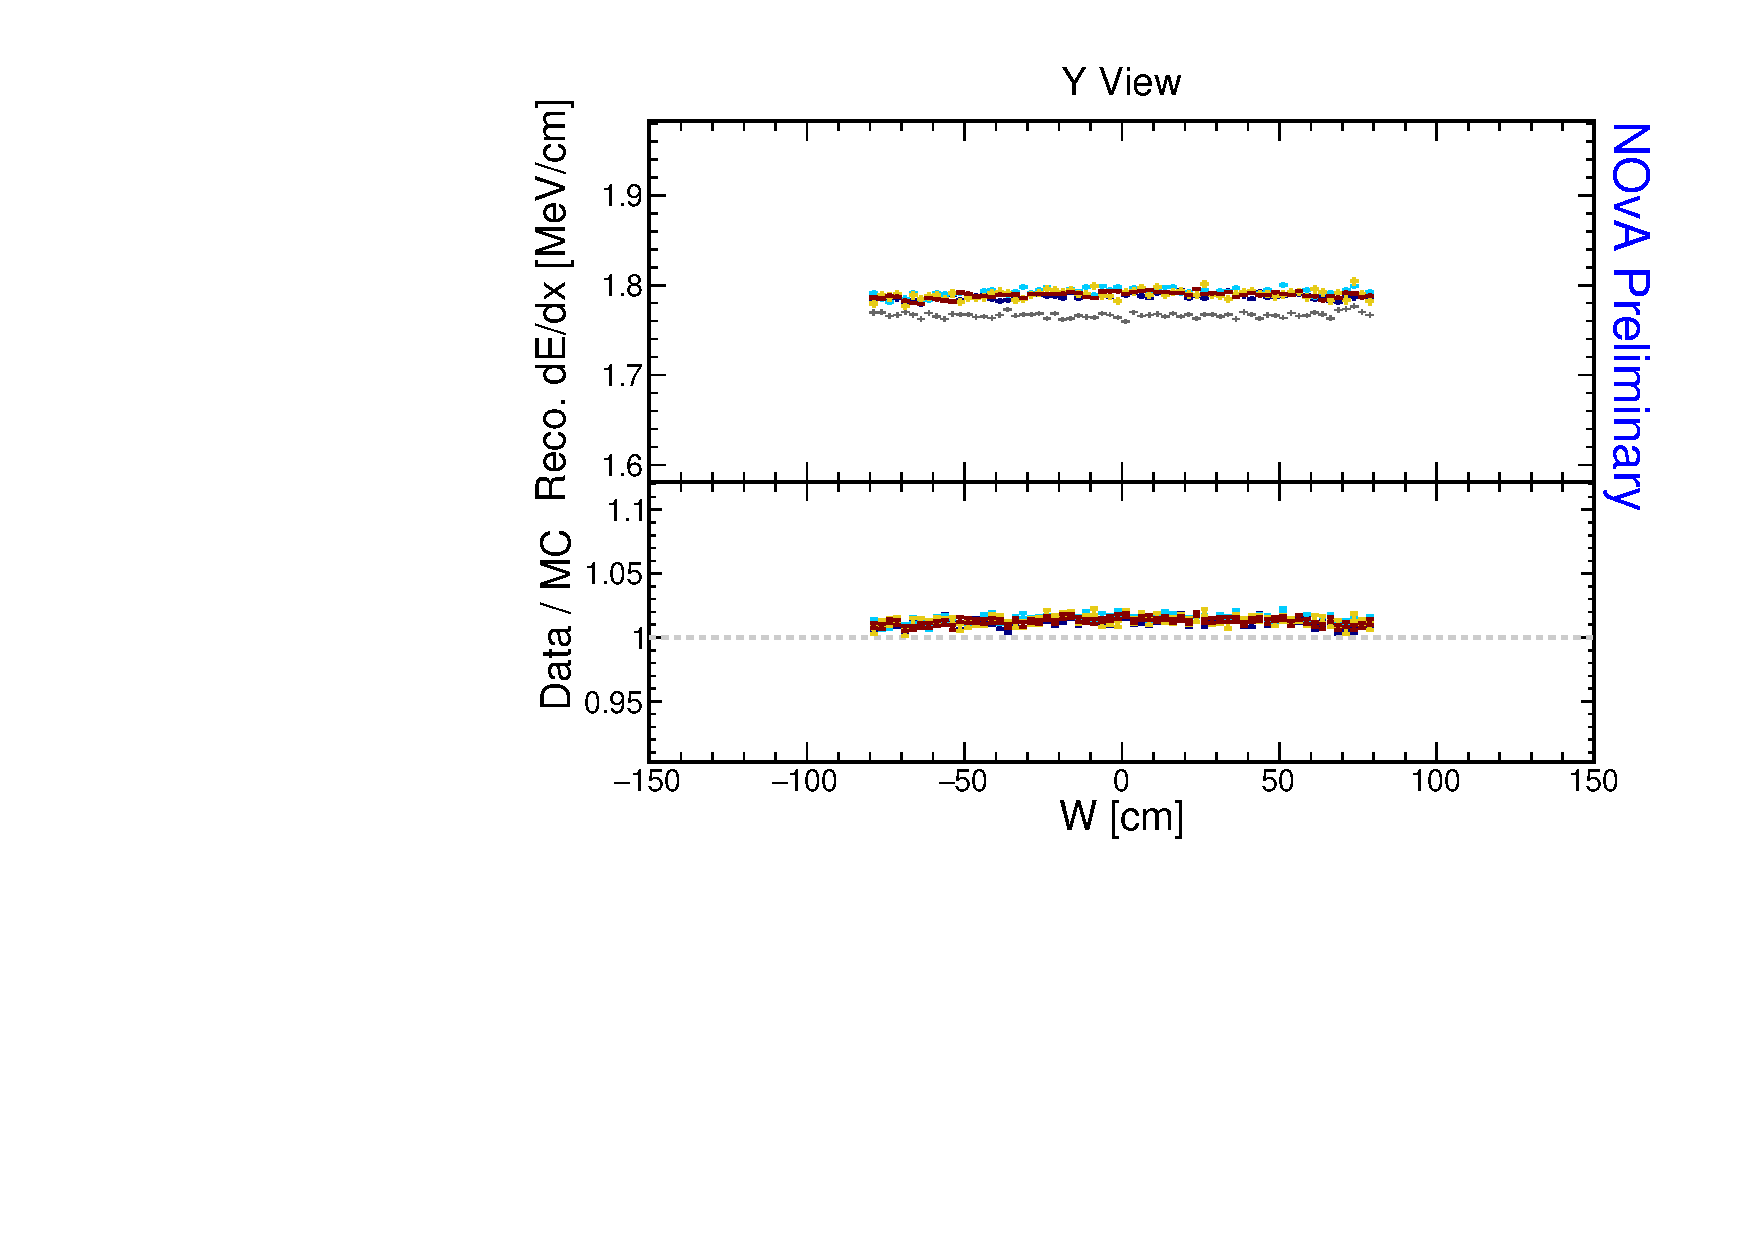
\includegraphics[width=\linewidth]{Plots/Calibana/recomevcm_w_y.pdf}
  \end{subfigure}
  \caption{Distributions of stopping muons within a 1-2 m track window from the end of their tracks across the position within a cell.}
  %\label{fig:AbsCalibW1}
\end{figure}

\begin{figure}[!ht]
  \begin{subfigure}{\textwidth}
  \centering
    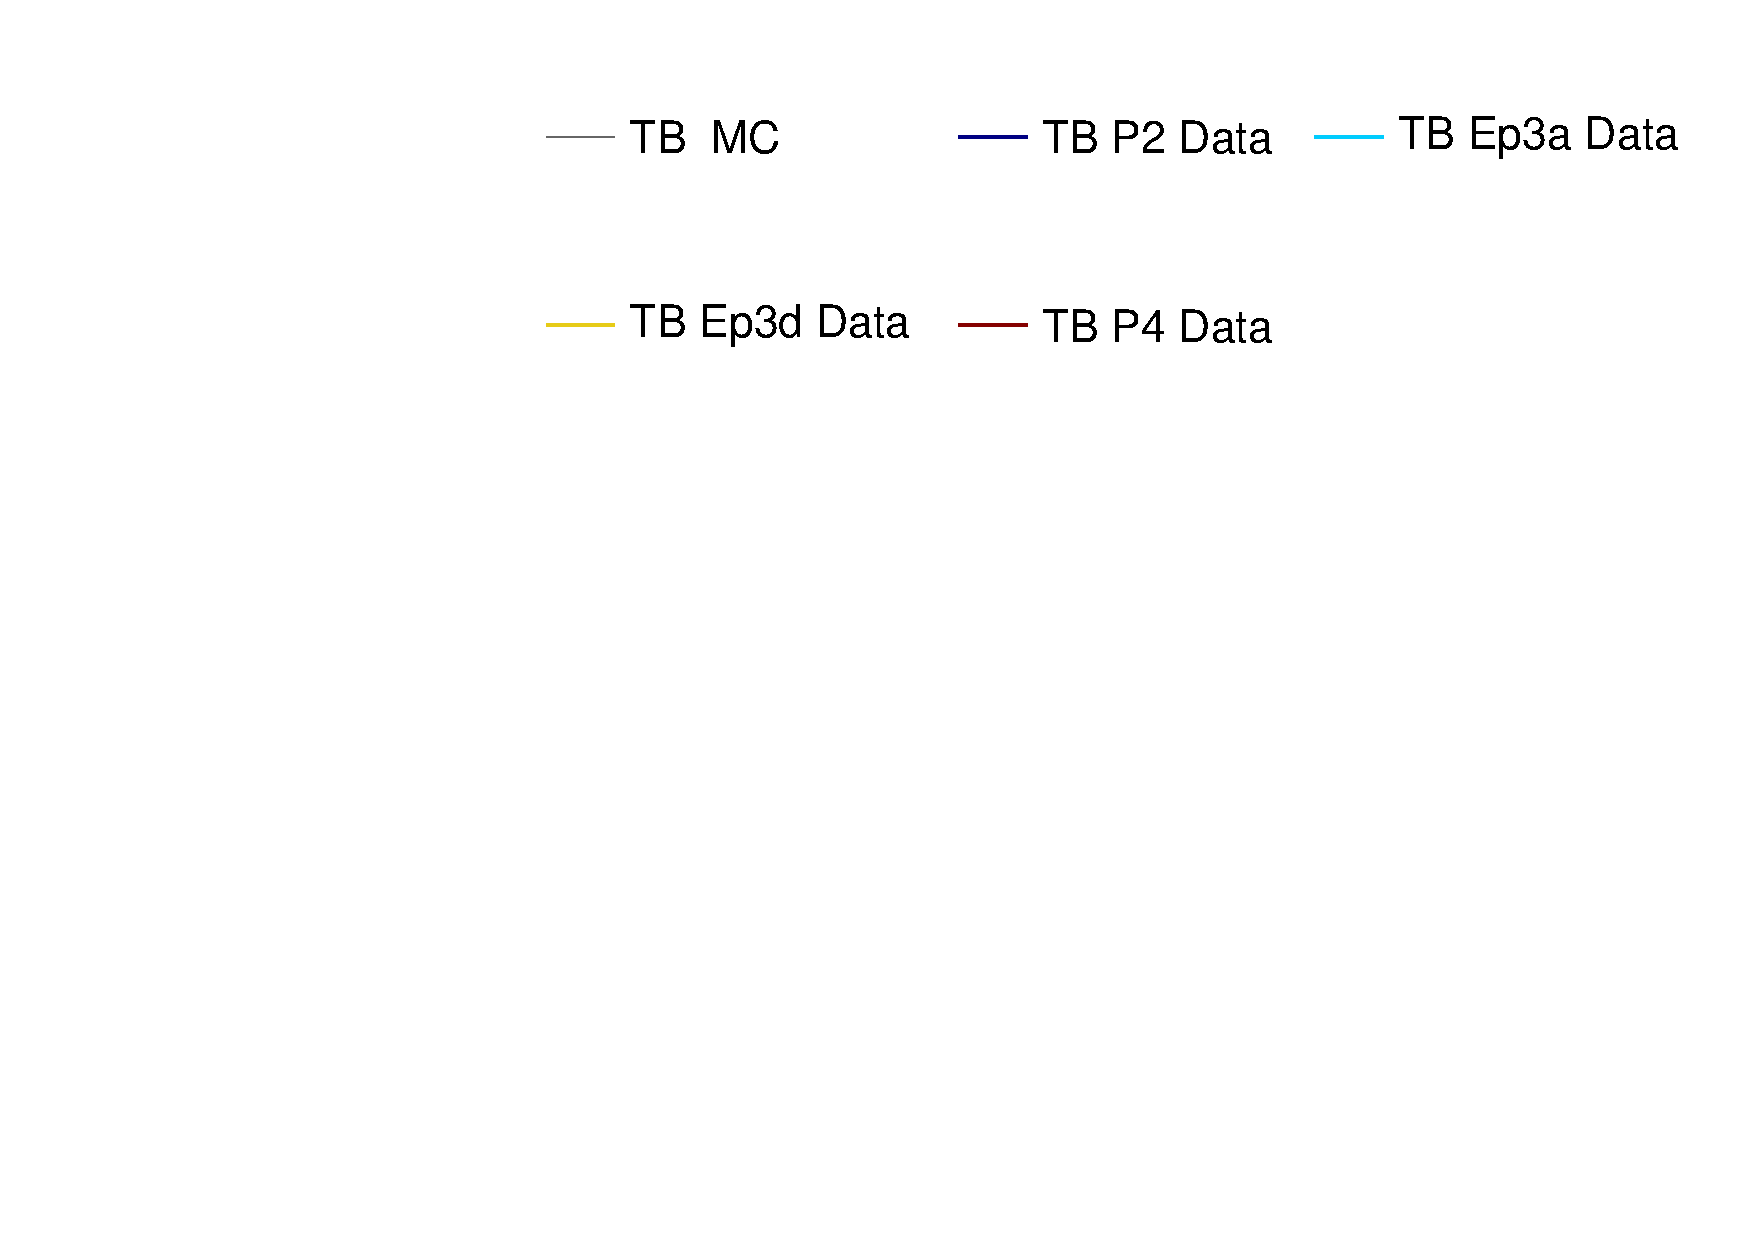
\includegraphics[height=0.2\linewidth]{Plots/Calibana/legend.pdf}
  \end{subfigure}
  \vspace*{2mm}

  \begin{subfigure}{0.495\textwidth}
    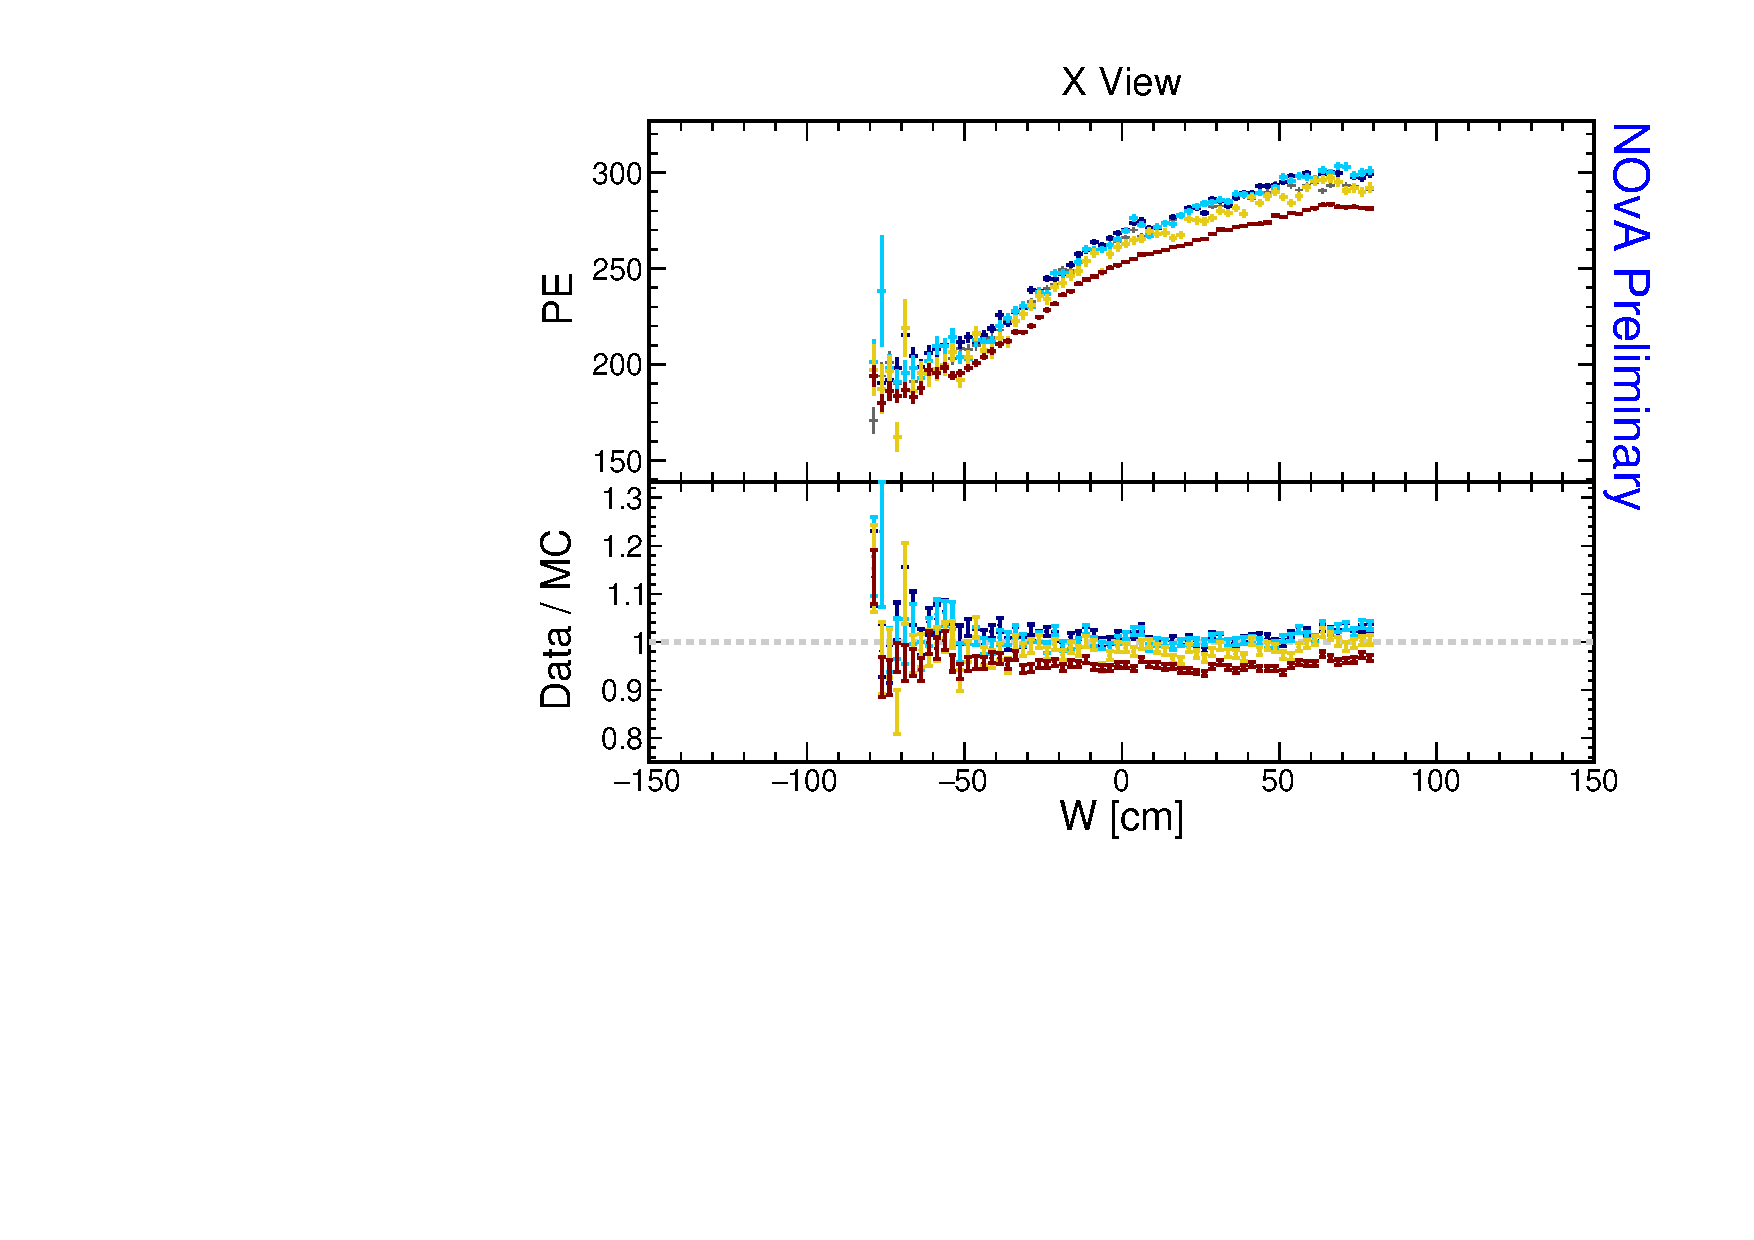
\includegraphics[width=\linewidth]{Plots/Calibana/pe_w_x.pdf}
  \end{subfigure}
  \begin{subfigure}{0.495\textwidth}
    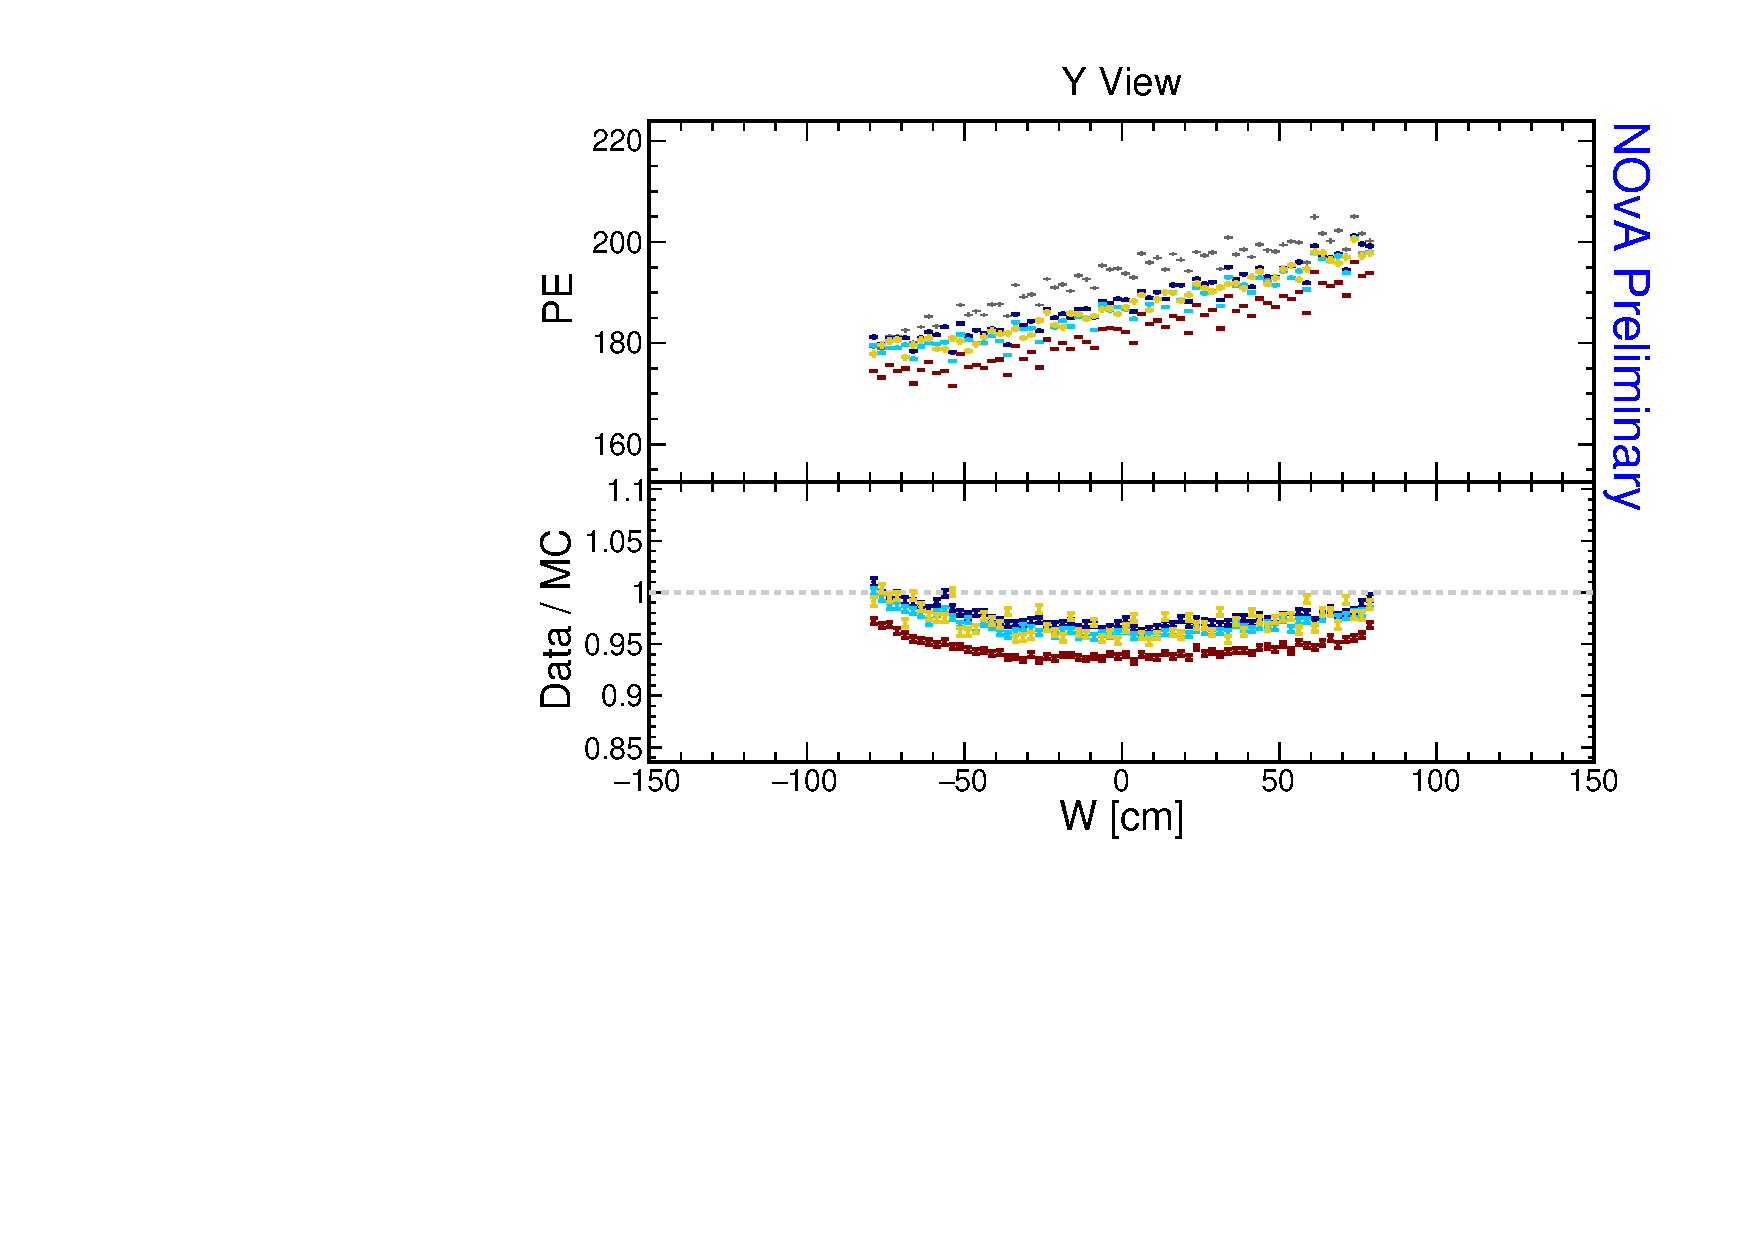
\includegraphics[width=\linewidth]{Plots/Calibana/pe_w_y.pdf}
  \end{subfigure}
  \begin{subfigure}{0.495\textwidth}
    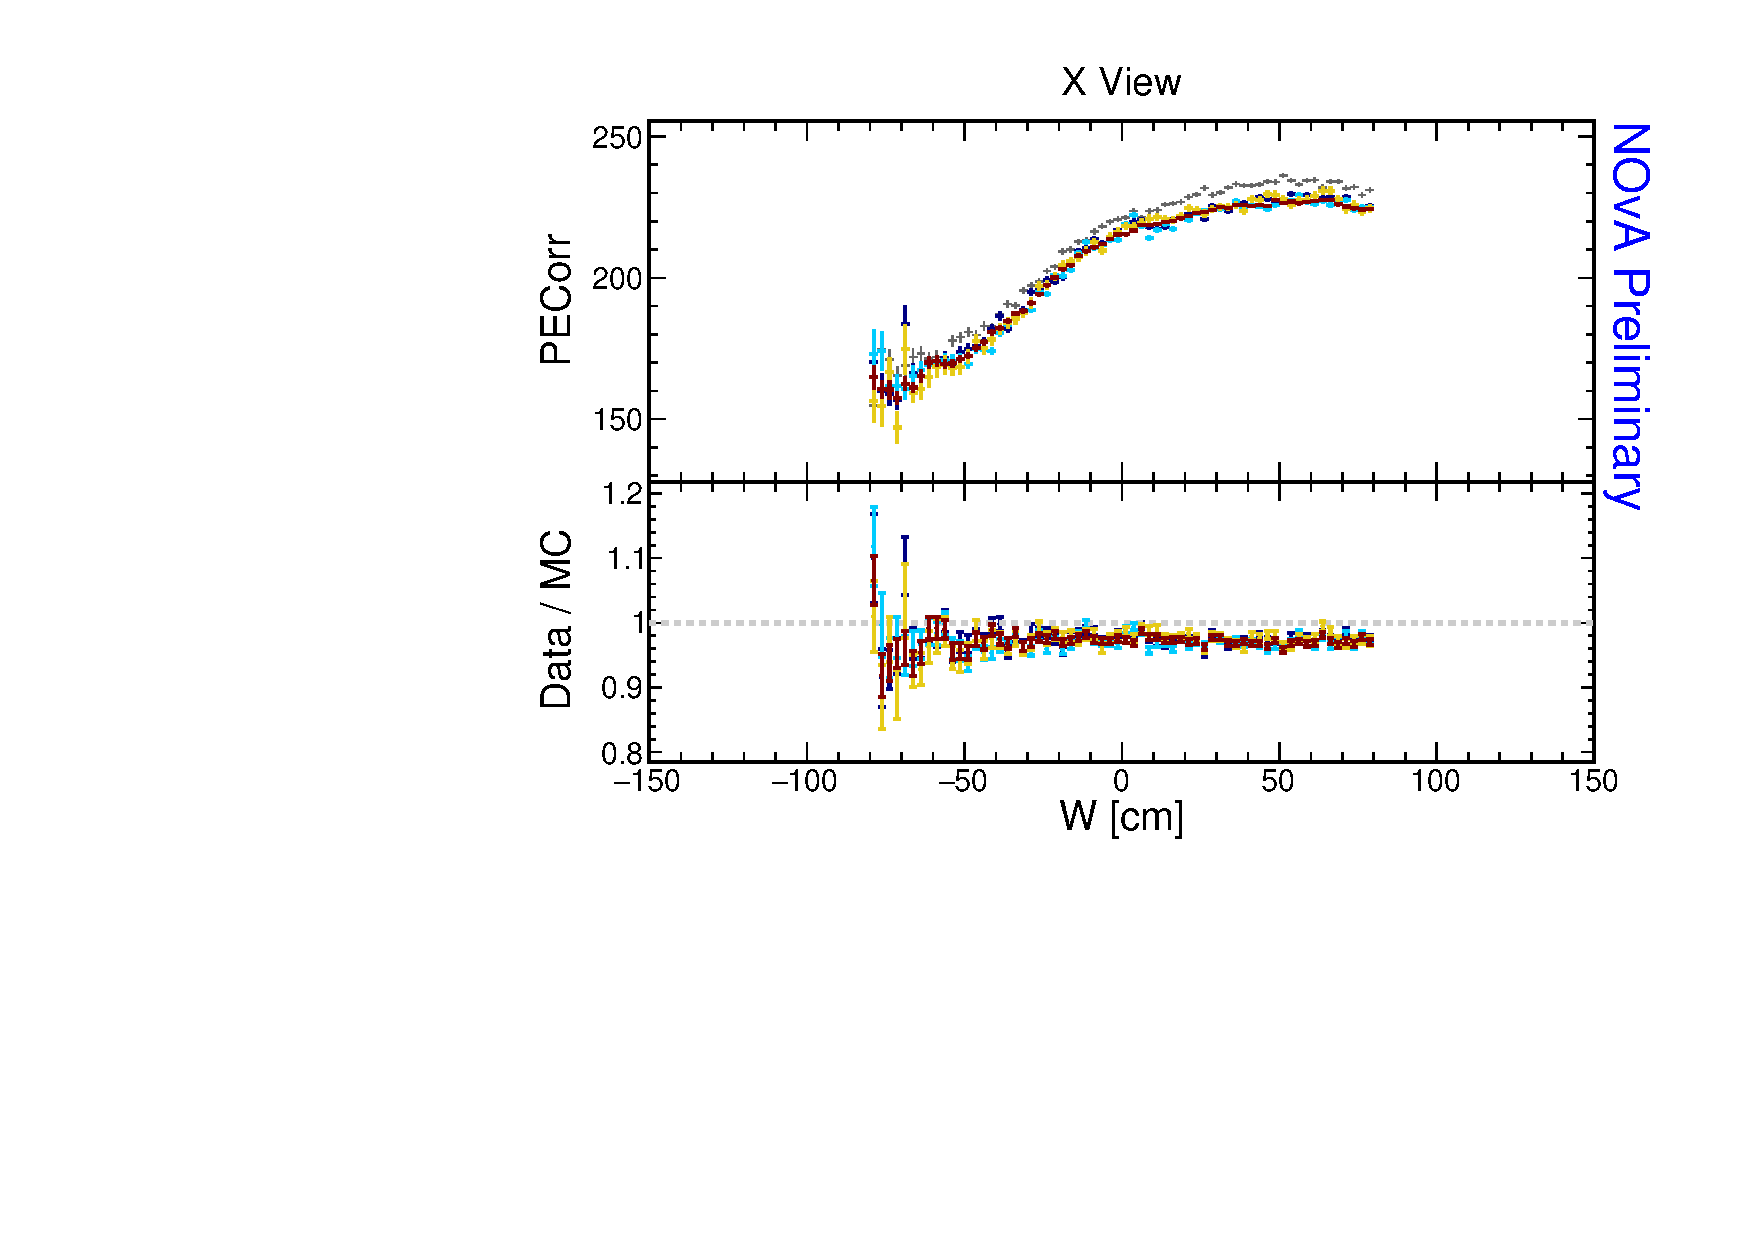
\includegraphics[width=\linewidth]{Plots/Calibana/pecorr_w_x.pdf}
  \end{subfigure}
  \begin{subfigure}{0.495\textwidth}
    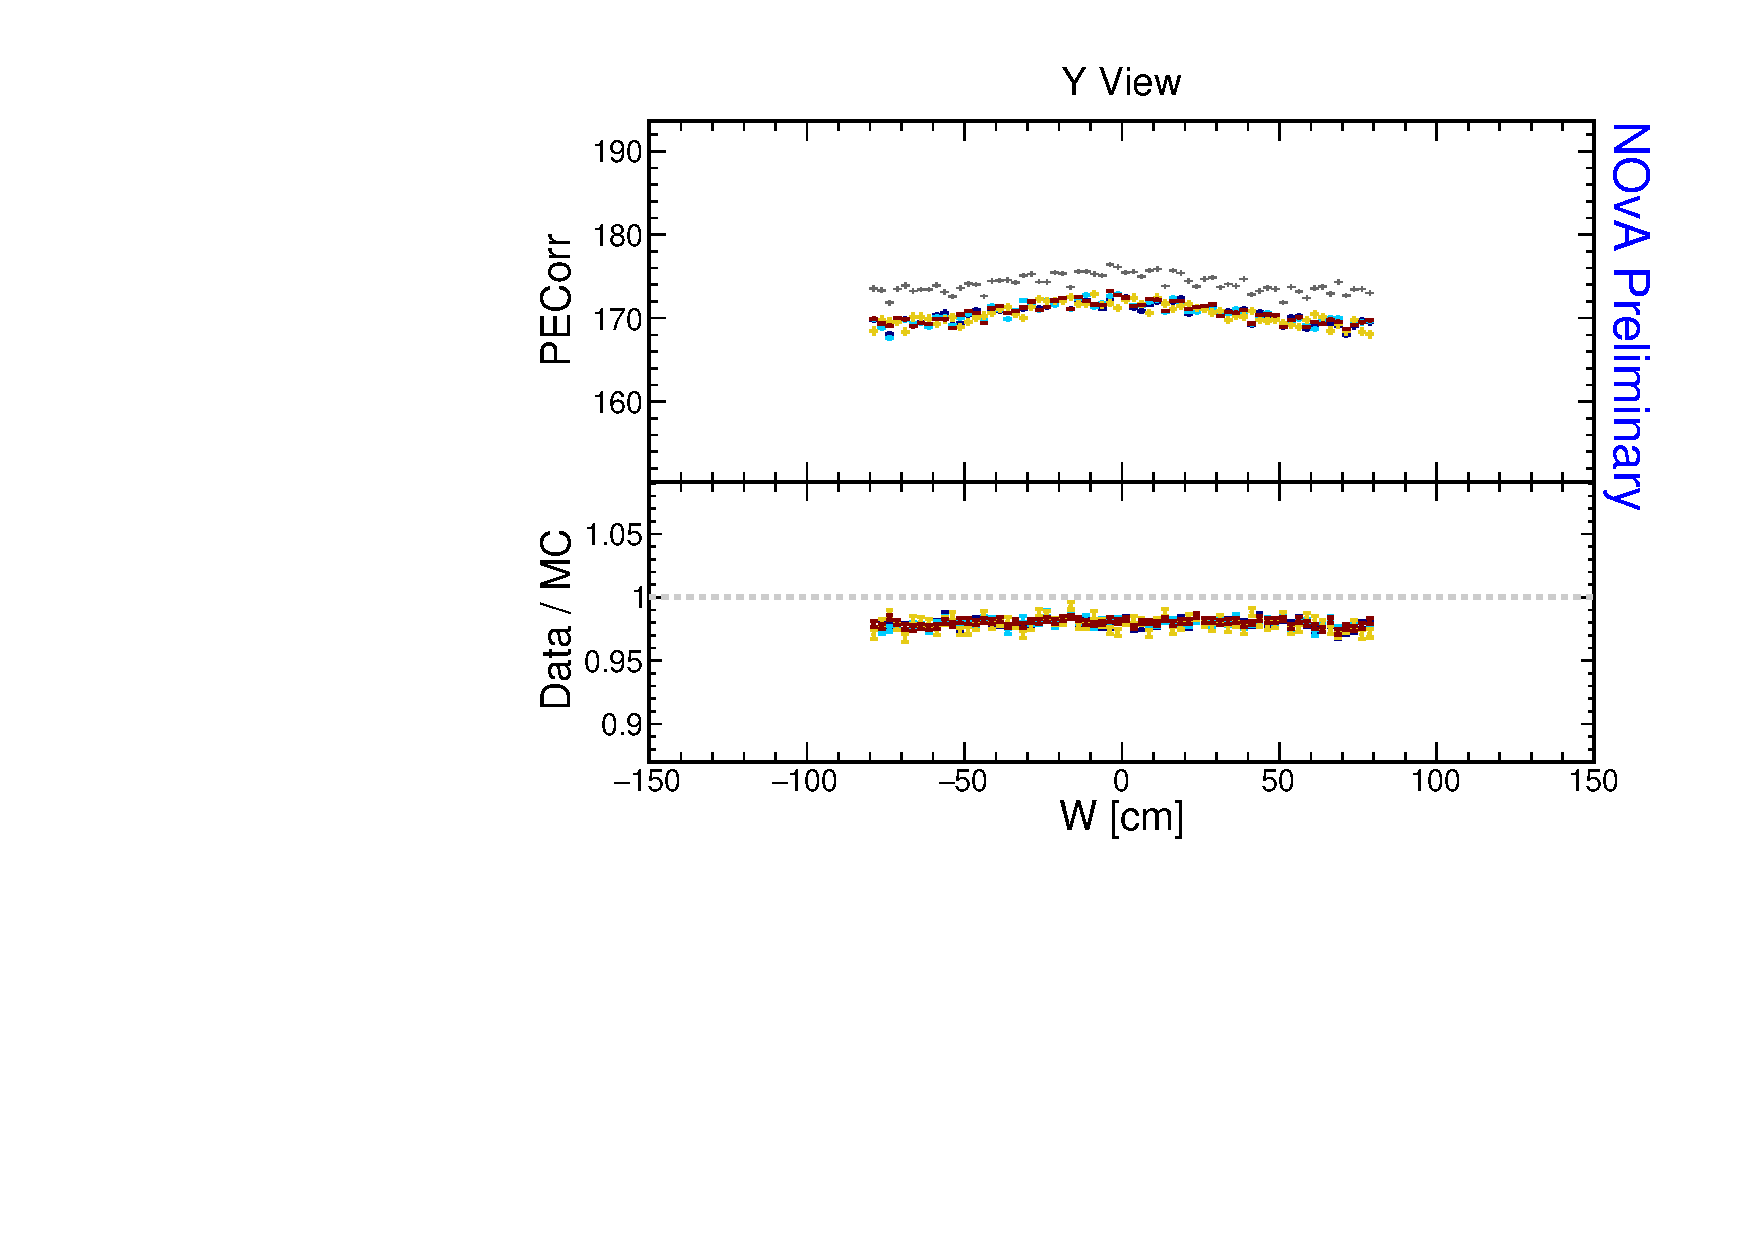
\includegraphics[width=\linewidth]{Plots/Calibana/pecorr_w_y.pdf}
  \end{subfigure}
  \begin{subfigure}{0.495\textwidth}
    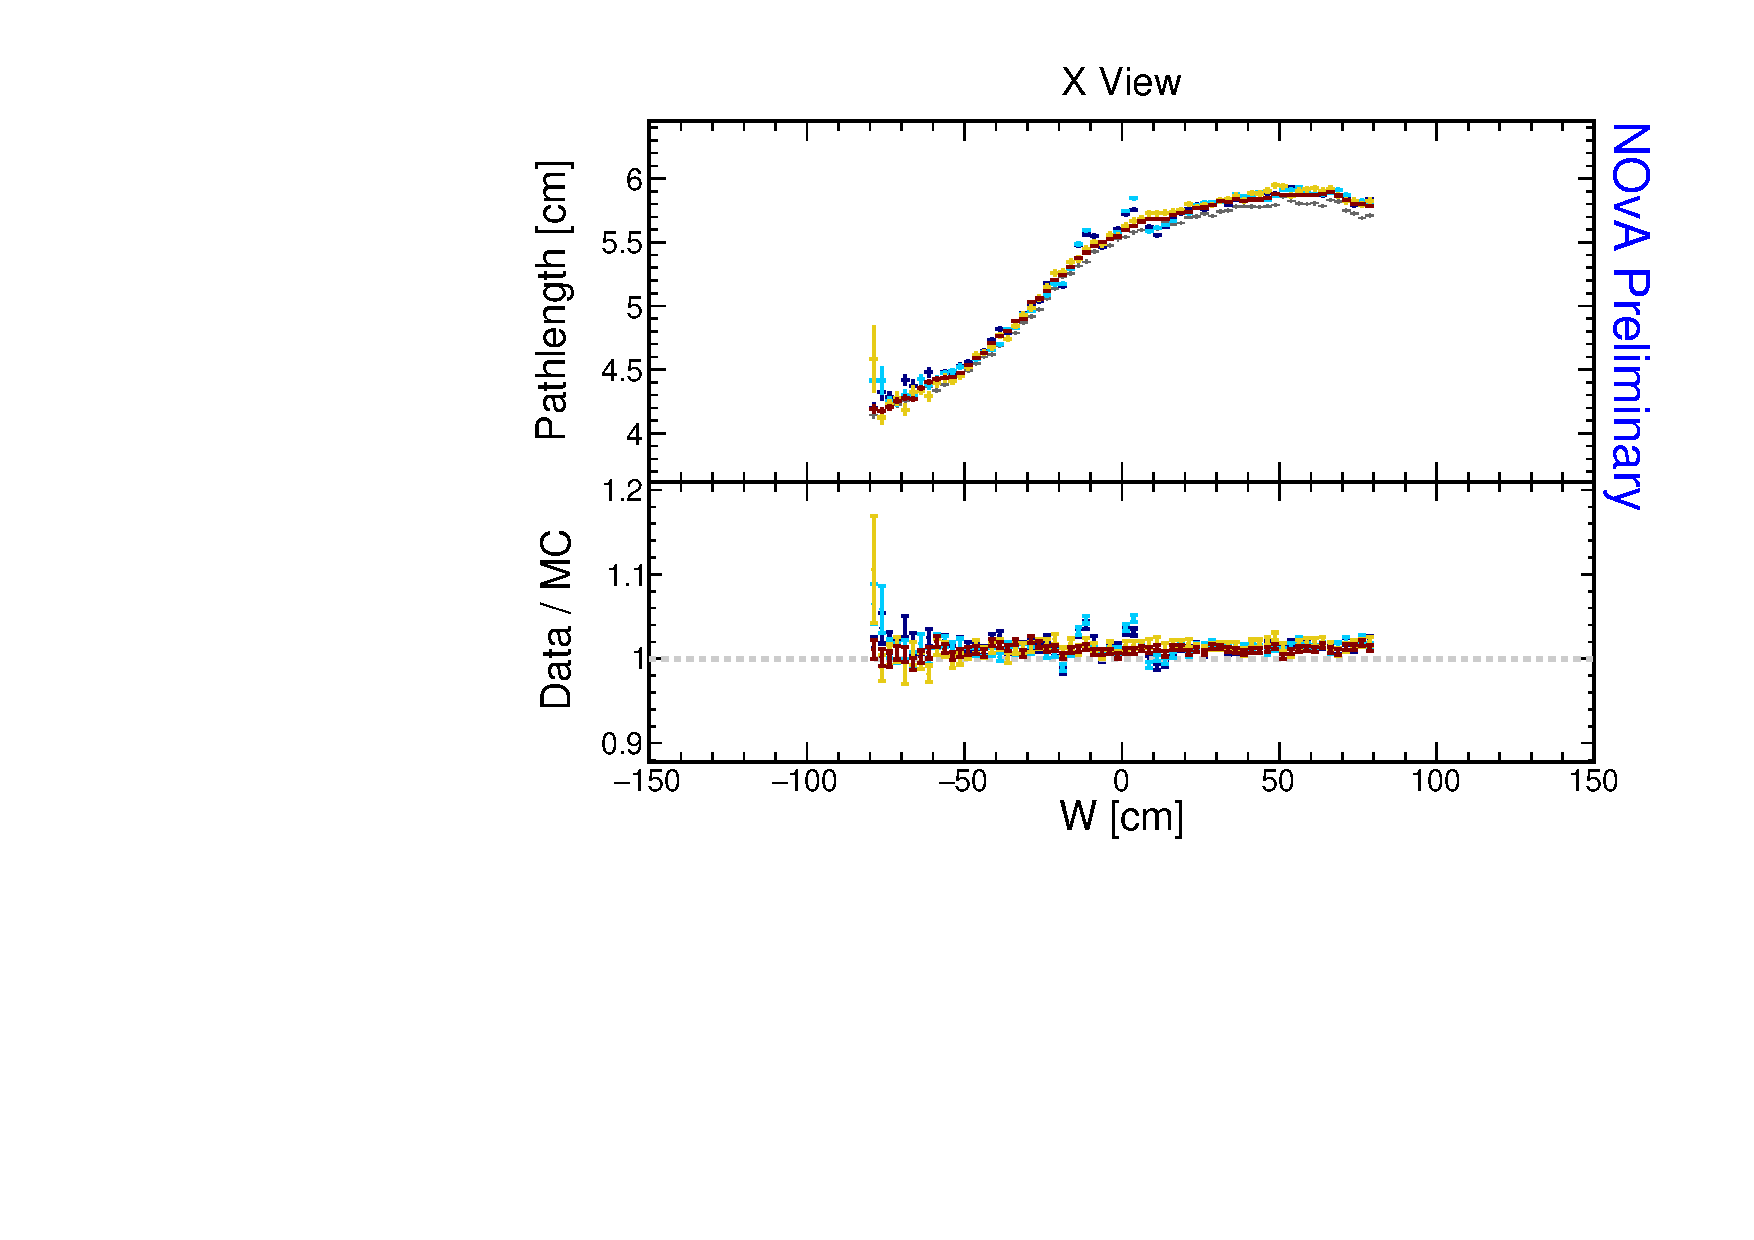
\includegraphics[width=\linewidth]{Plots/Calibana/cm_w_x.pdf}
  \end{subfigure}
  \begin{subfigure}{0.495\textwidth}
    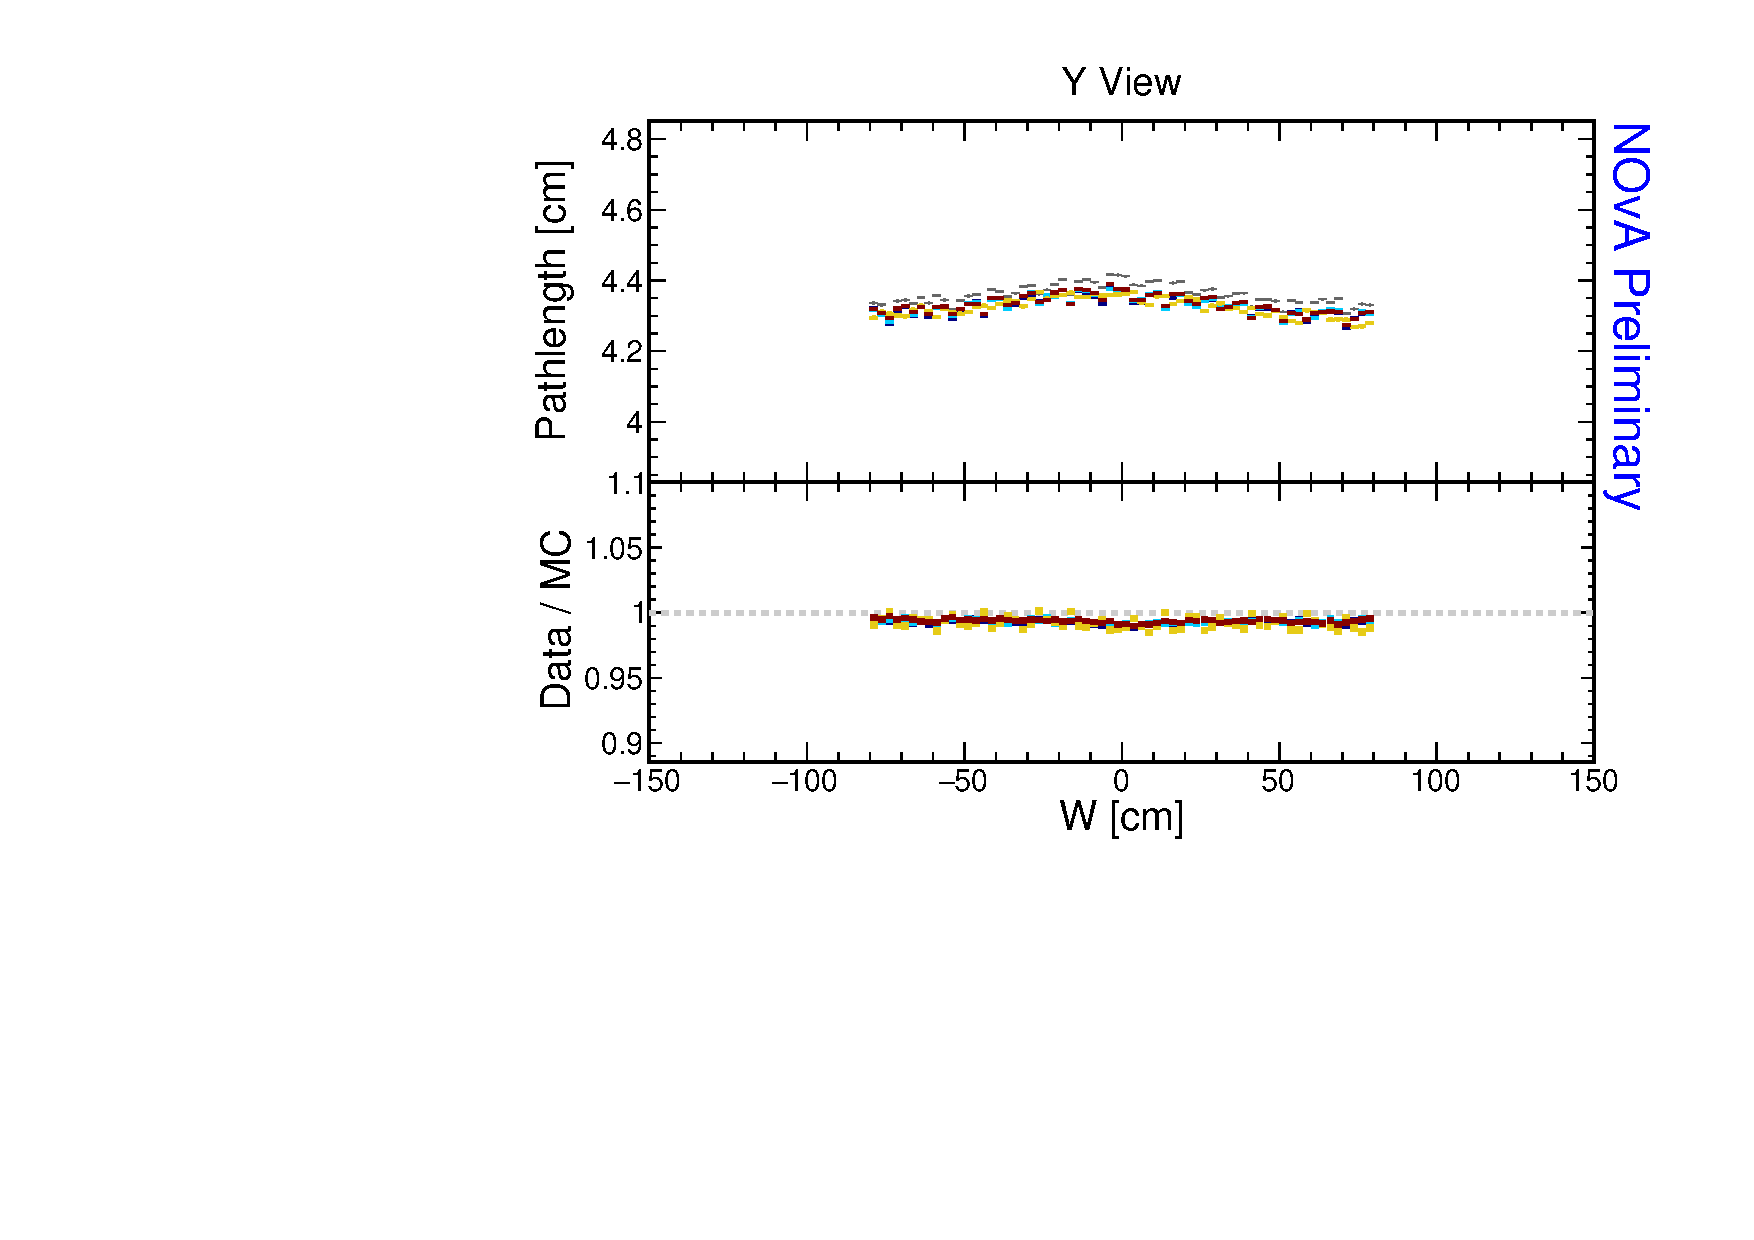
\includegraphics[width=\linewidth]{Plots/Calibana/cm_w_y.pdf}
  \end{subfigure}
  \caption{Distributions of stopping muons within a 1-2 m track window from the end of their tracks across the position within a cell.}
  %\label{fig:AbsCalibW2}
\end{figure}

\begin{figure}[!ht]
  \begin{subfigure}{\textwidth}
  \centering
    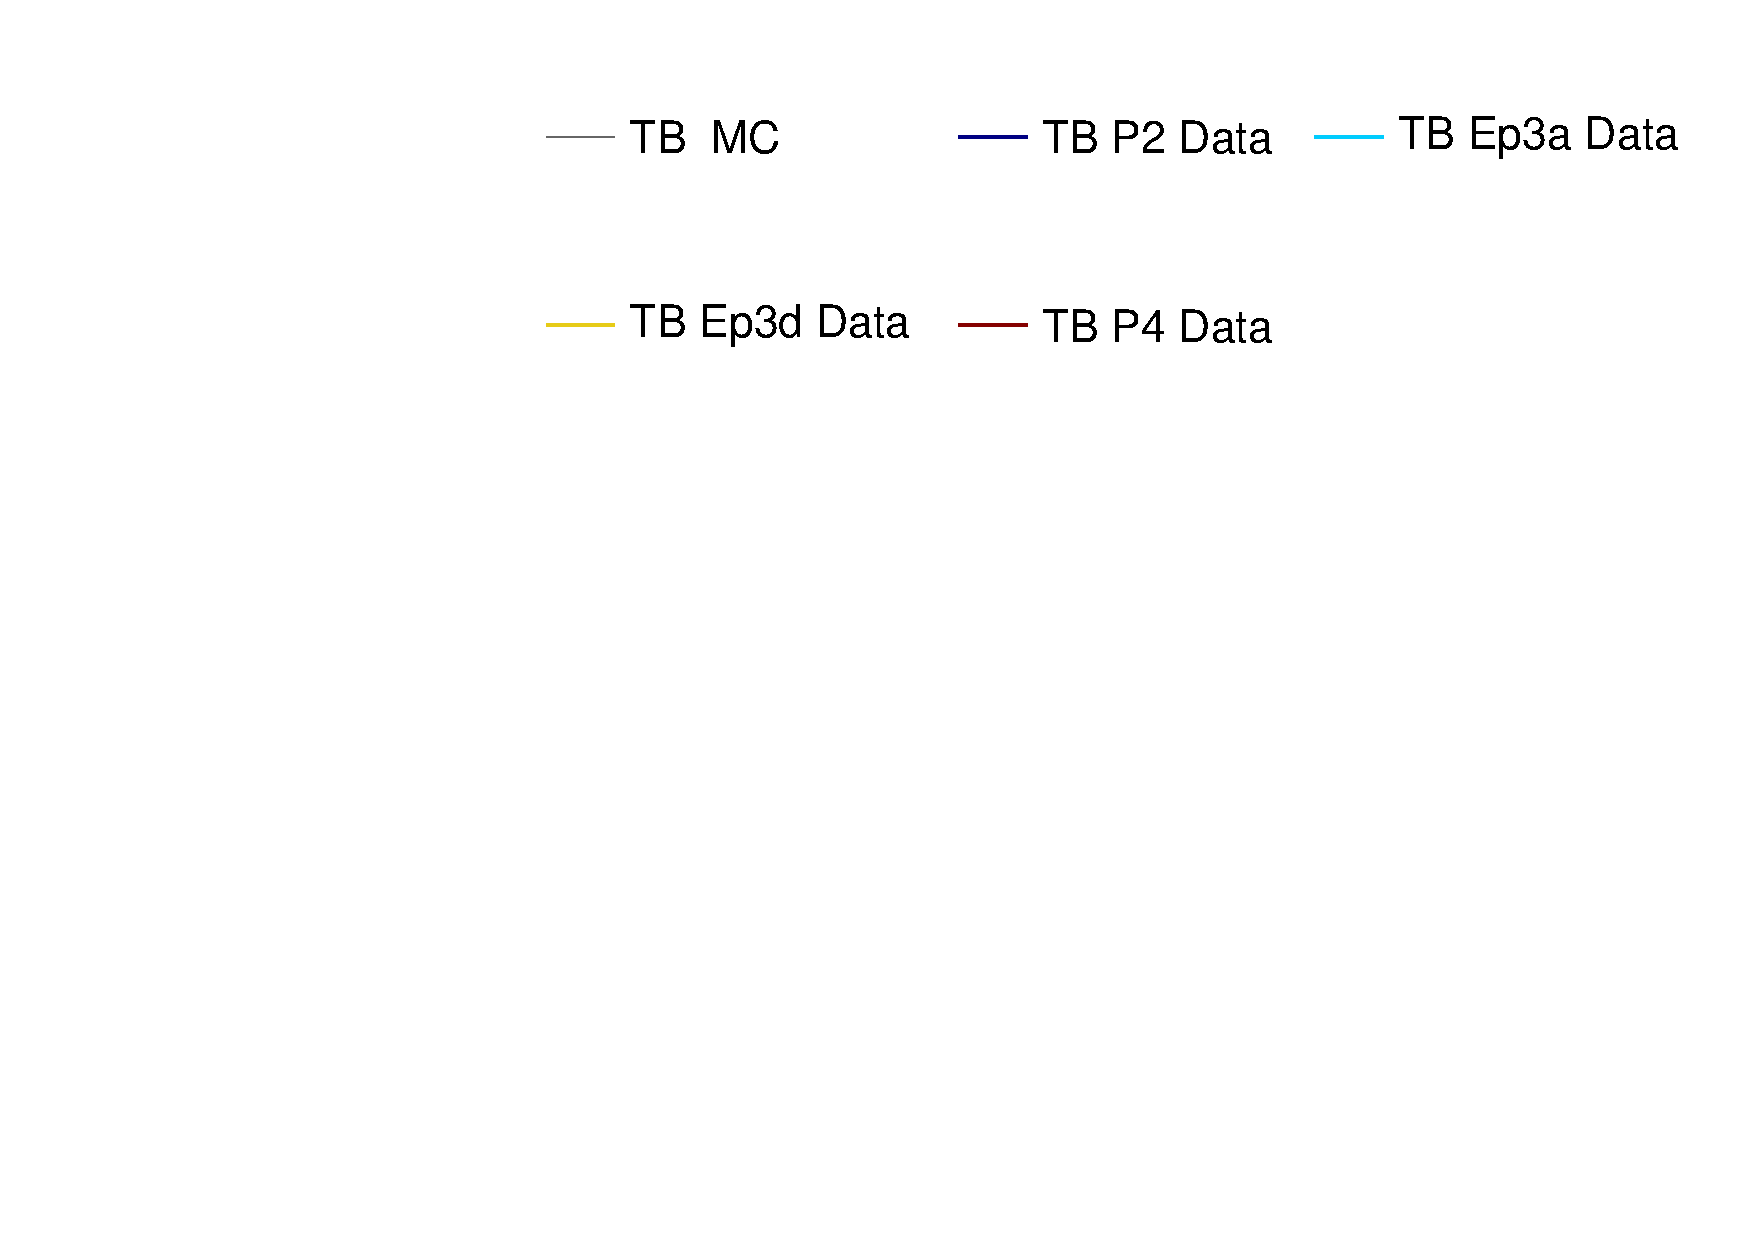
\includegraphics[height=0.2\linewidth]{Plots/Calibana/legend.pdf}
  \end{subfigure}
  \vspace*{2mm}

  \begin{subfigure}{0.495\textwidth}
    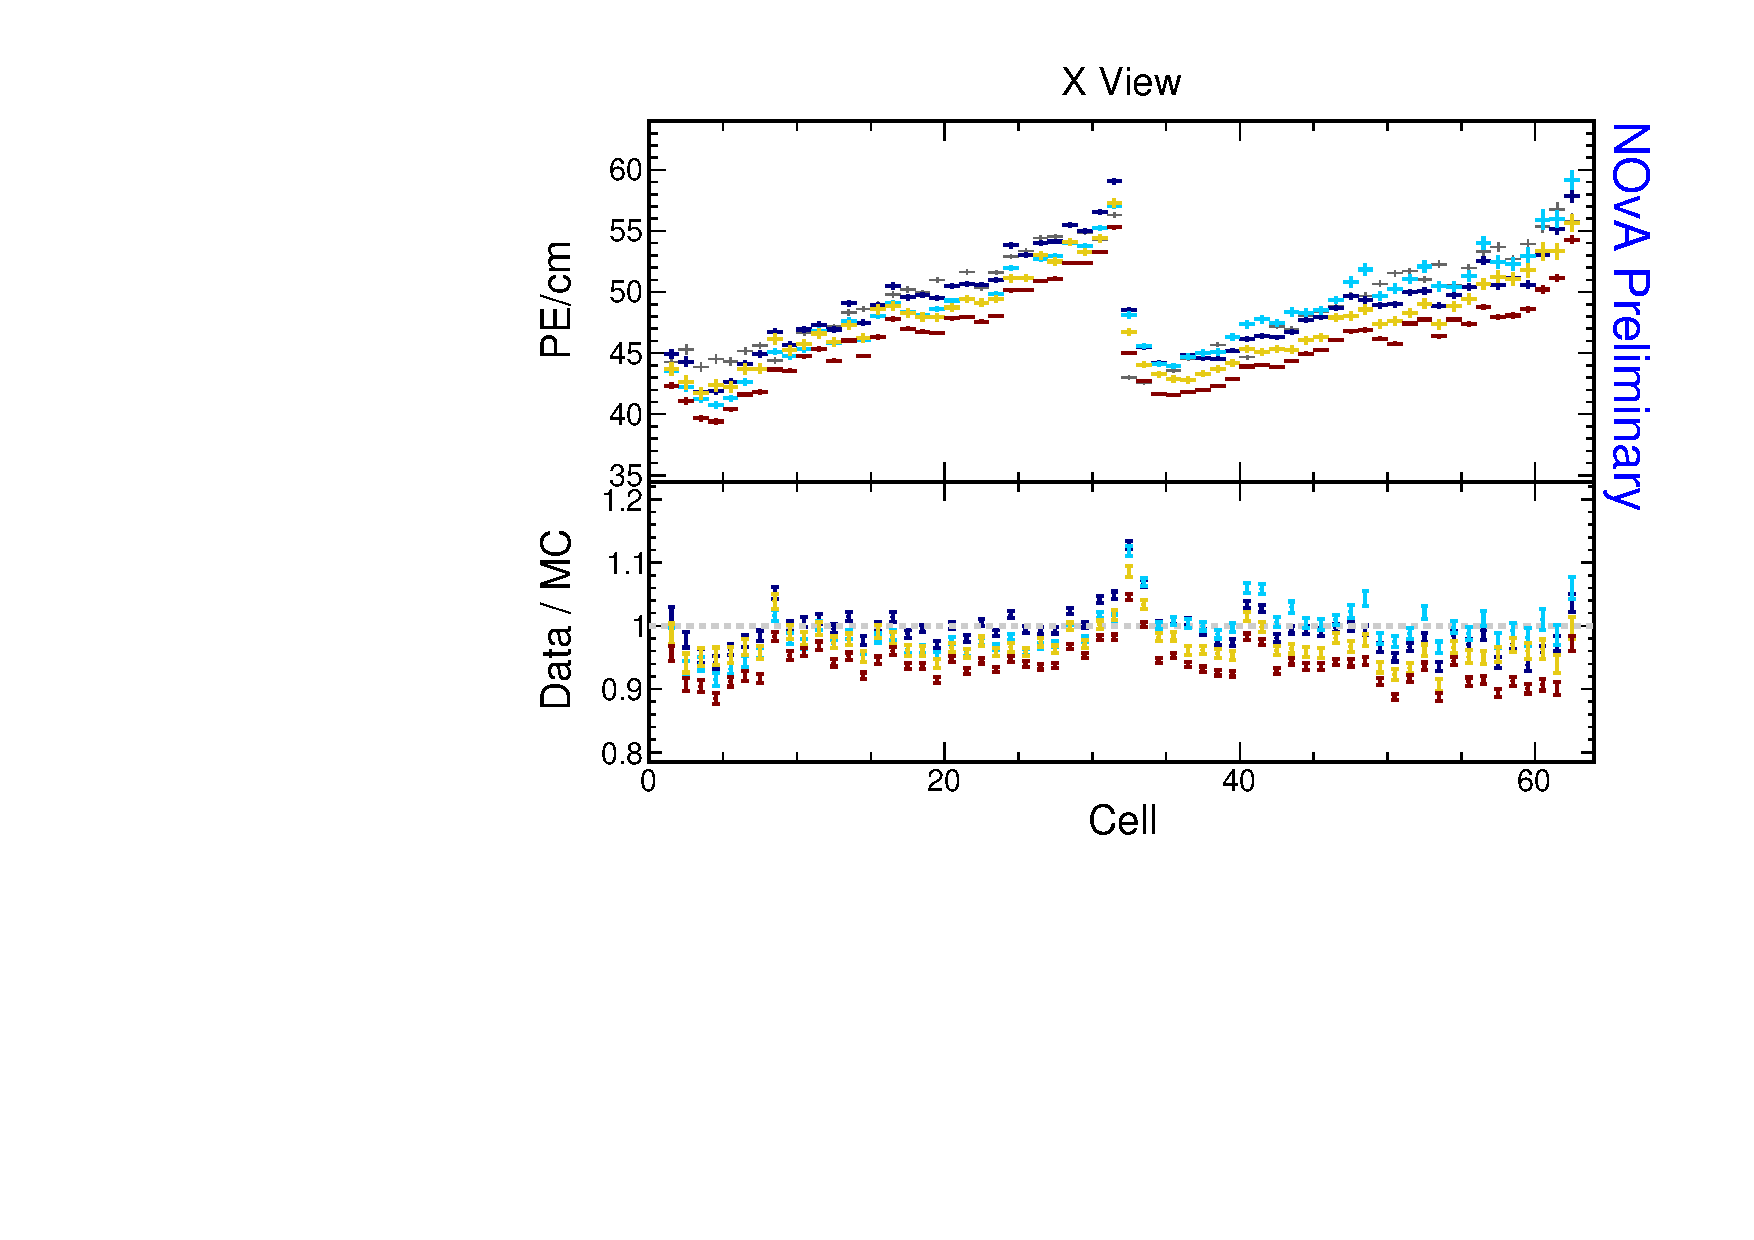
\includegraphics[width=\linewidth]{Plots/Calibana/pecm_cell_x.pdf}
  \end{subfigure}
  \begin{subfigure}{0.495\textwidth}
    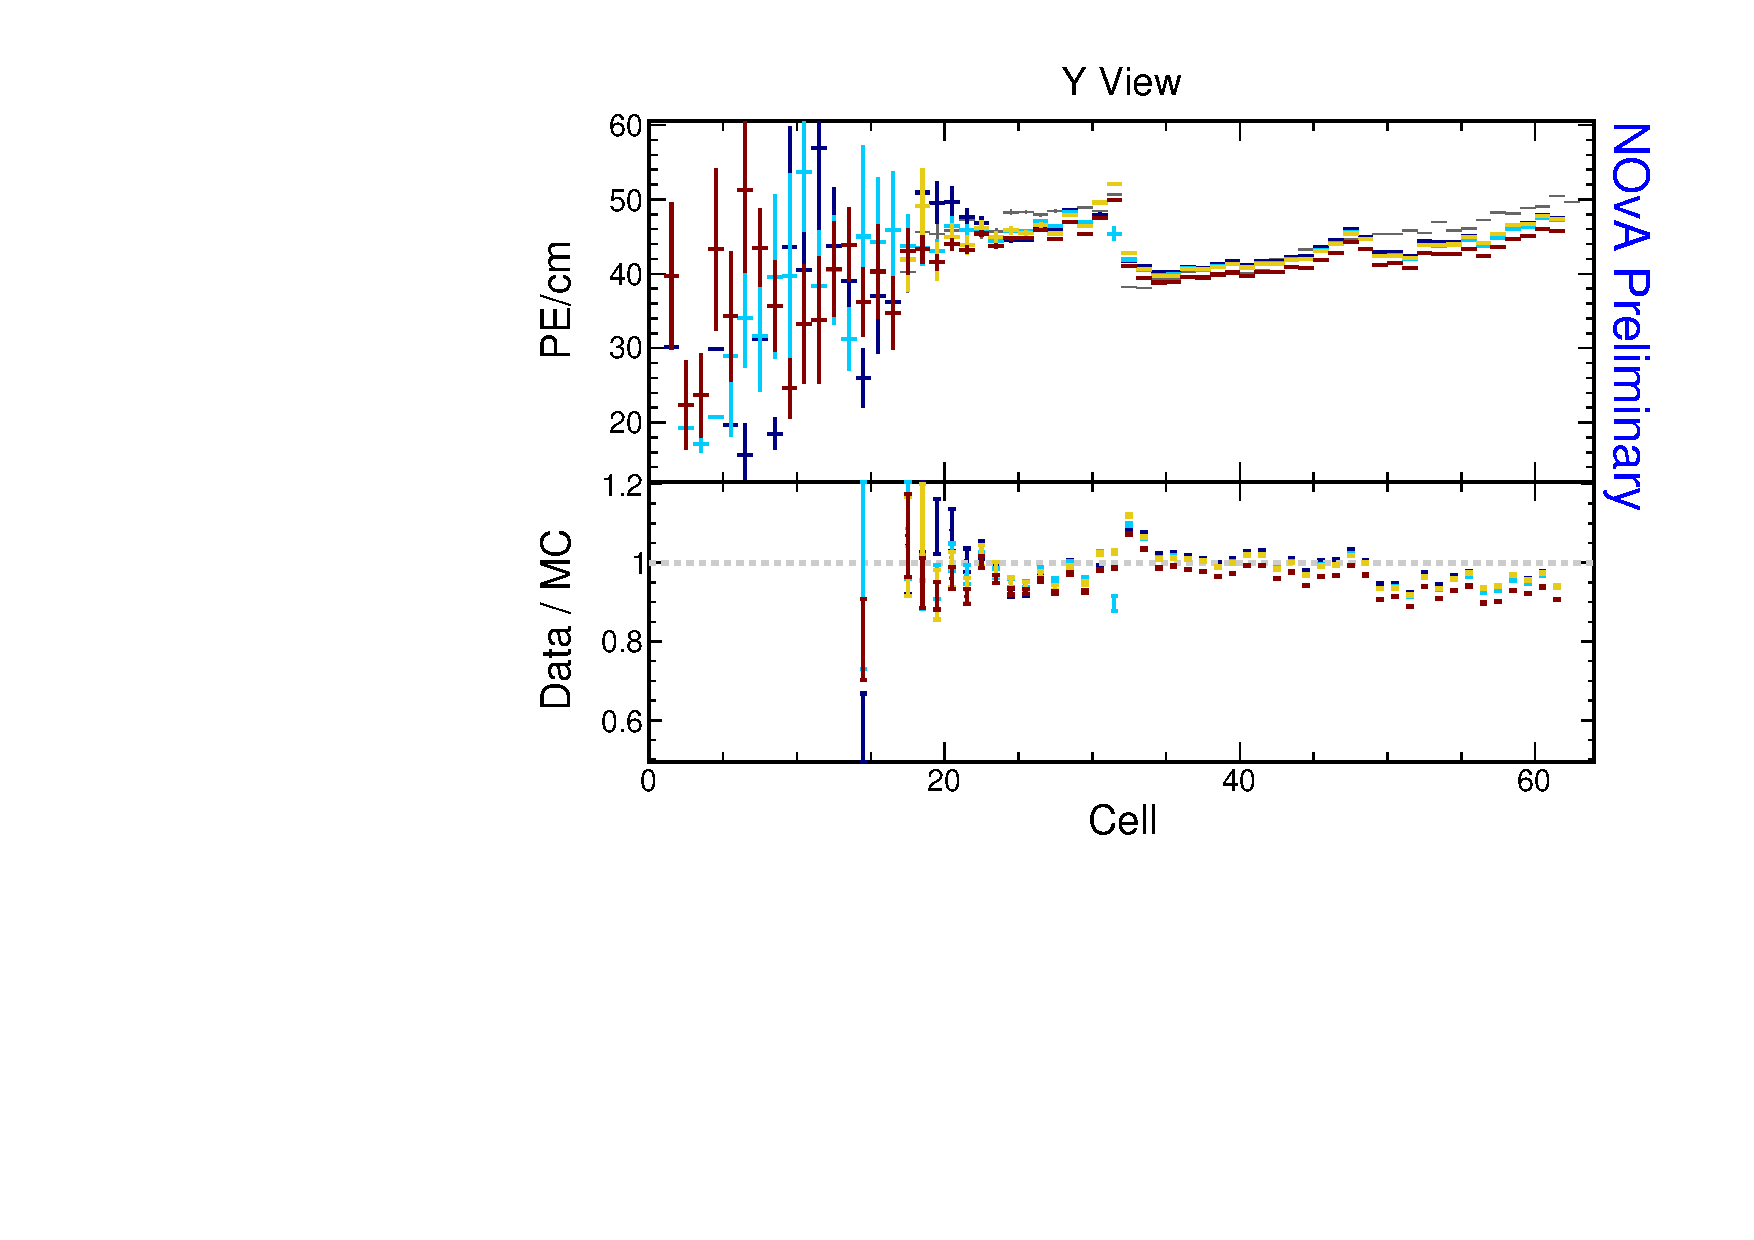
\includegraphics[width=\linewidth]{Plots/Calibana/pecm_cell_y.pdf}
  \end{subfigure}
  \begin{subfigure}{0.495\textwidth}
    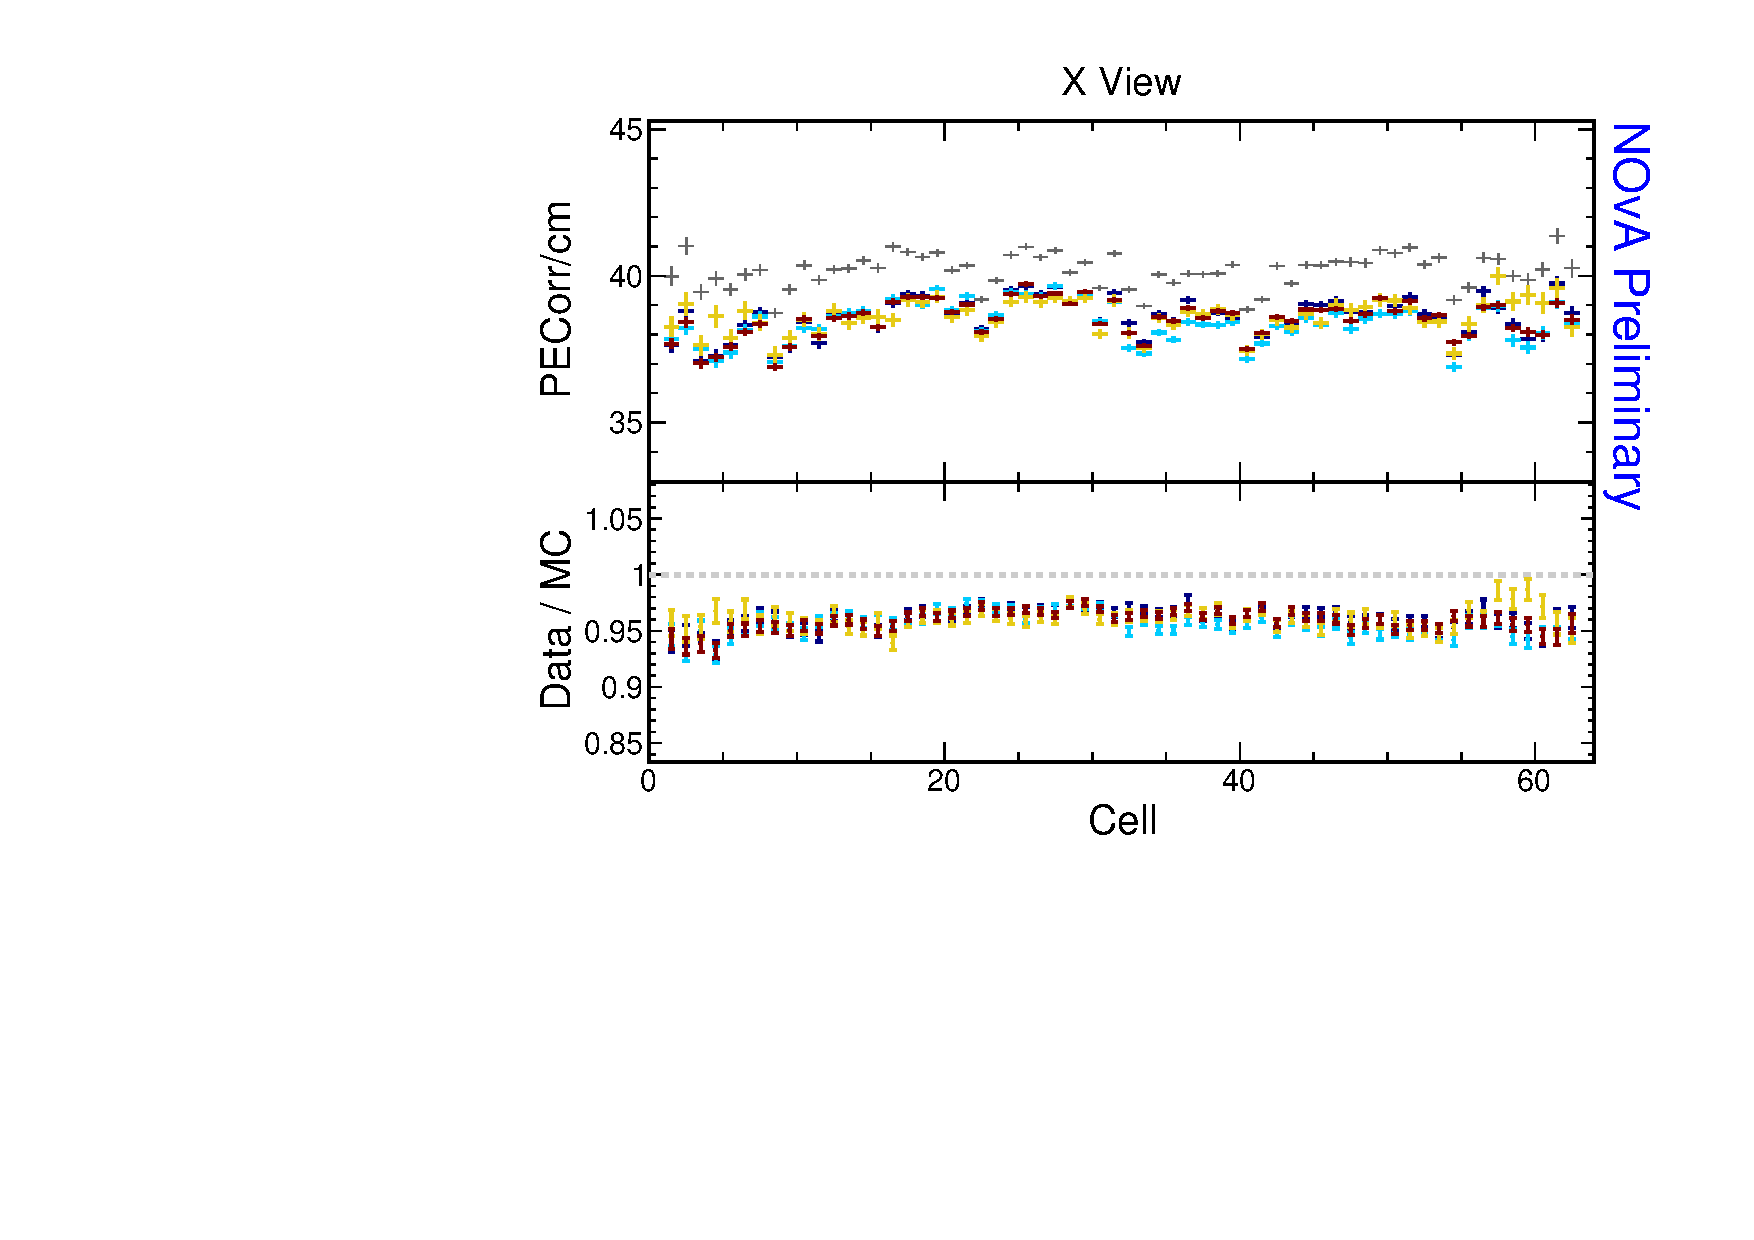
\includegraphics[width=\linewidth]{Plots/Calibana/pecorrcm_cell_x.pdf}
  \end{subfigure}
  \begin{subfigure}{0.495\textwidth}
    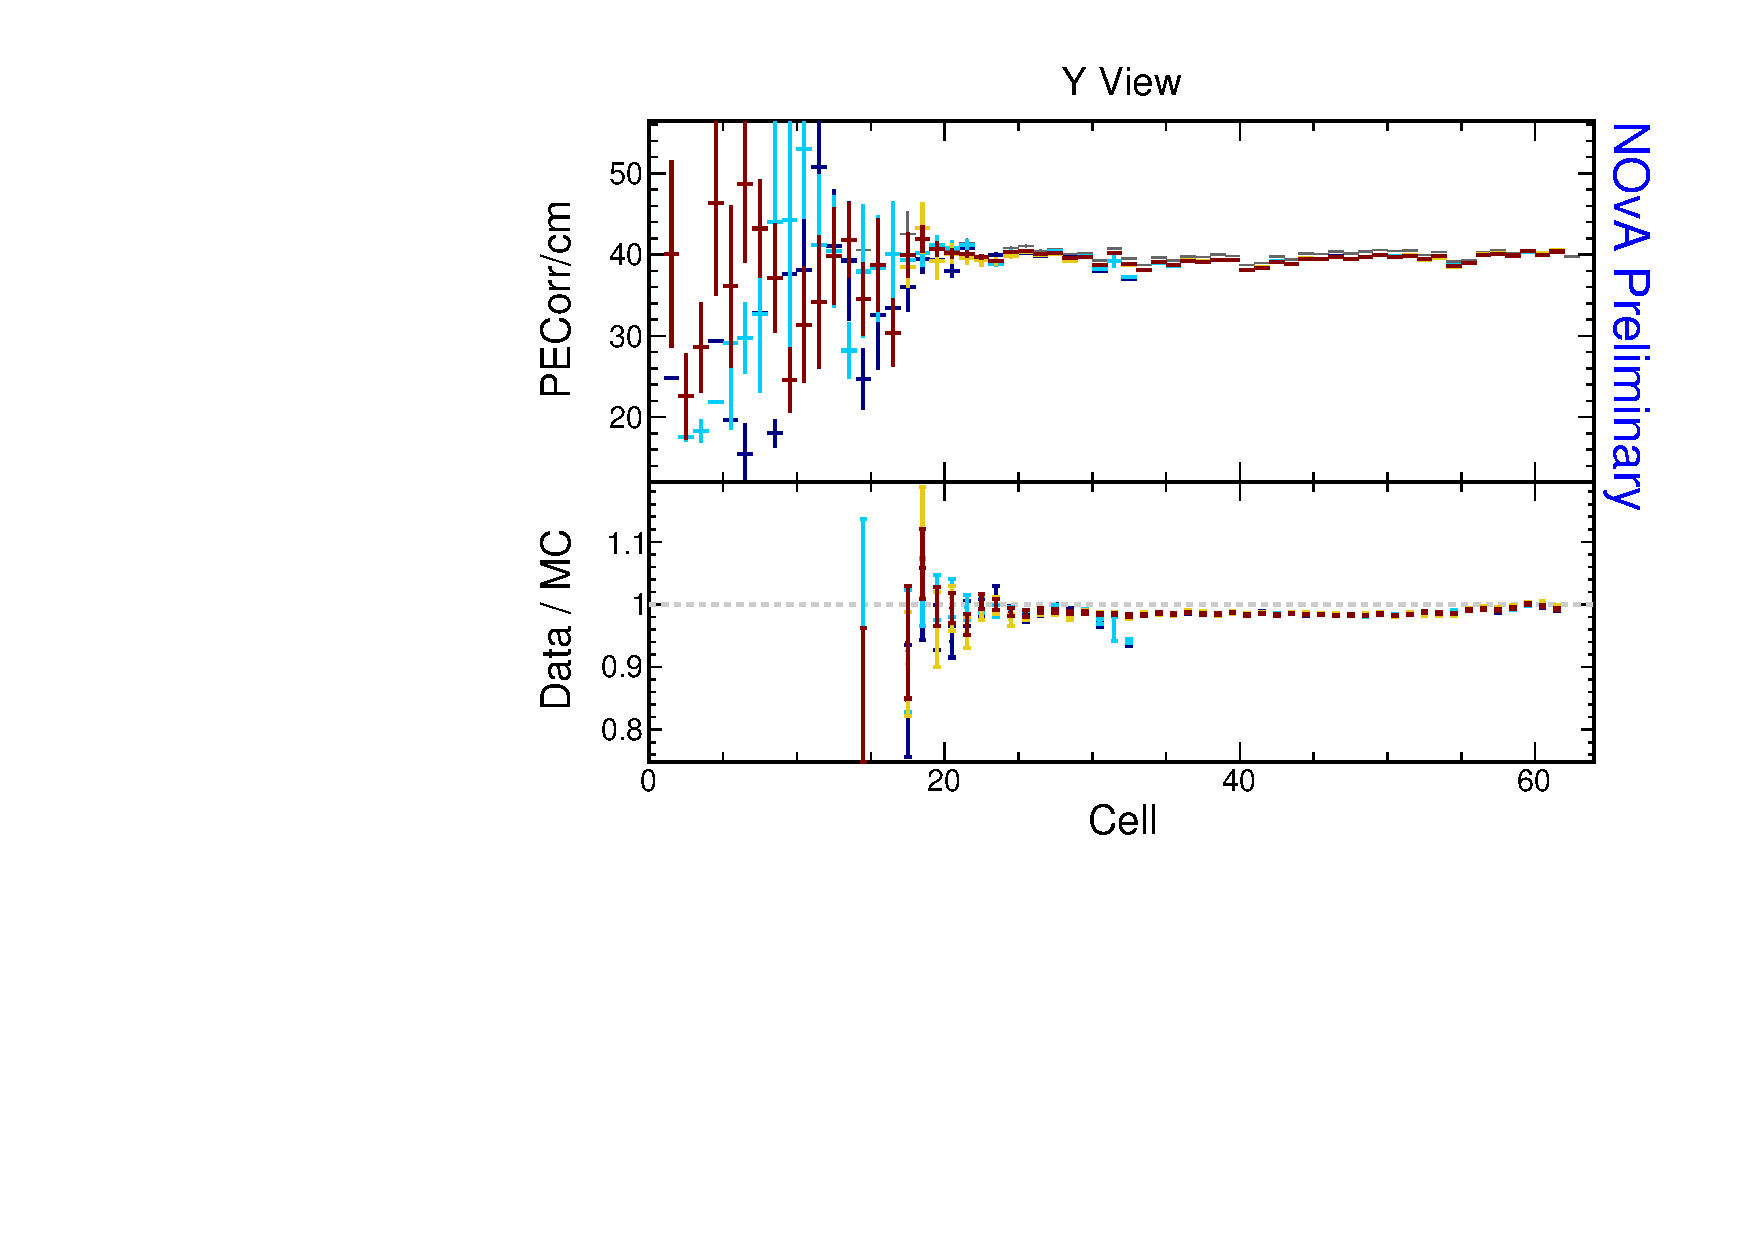
\includegraphics[width=\linewidth]{Plots/Calibana/pecorrcm_cell_y.pdf}
  \end{subfigure}
    \begin{subfigure}{0.495\textwidth}
    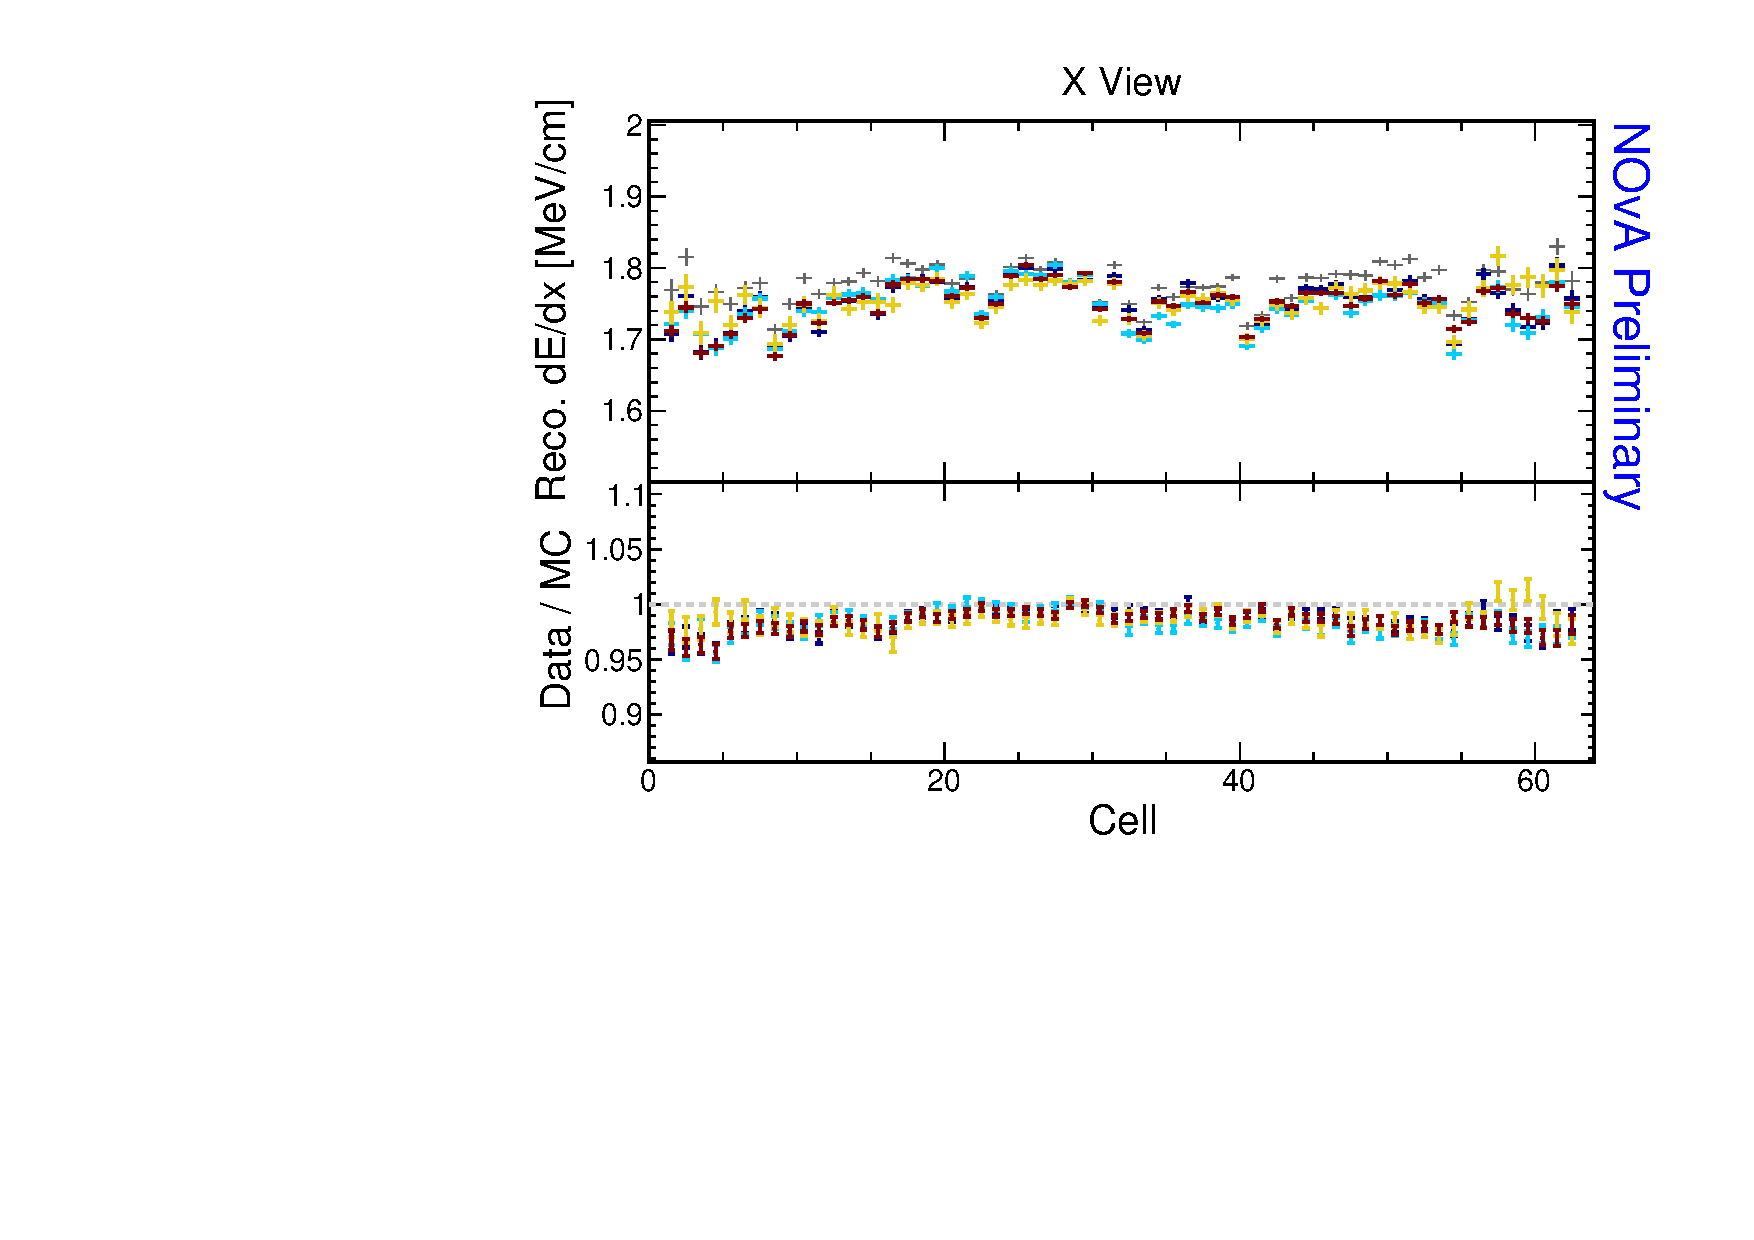
\includegraphics[width=\linewidth]{Plots/Calibana/recomevcm_cell_x.pdf}
  \end{subfigure}
  \begin{subfigure}{0.495\textwidth}
    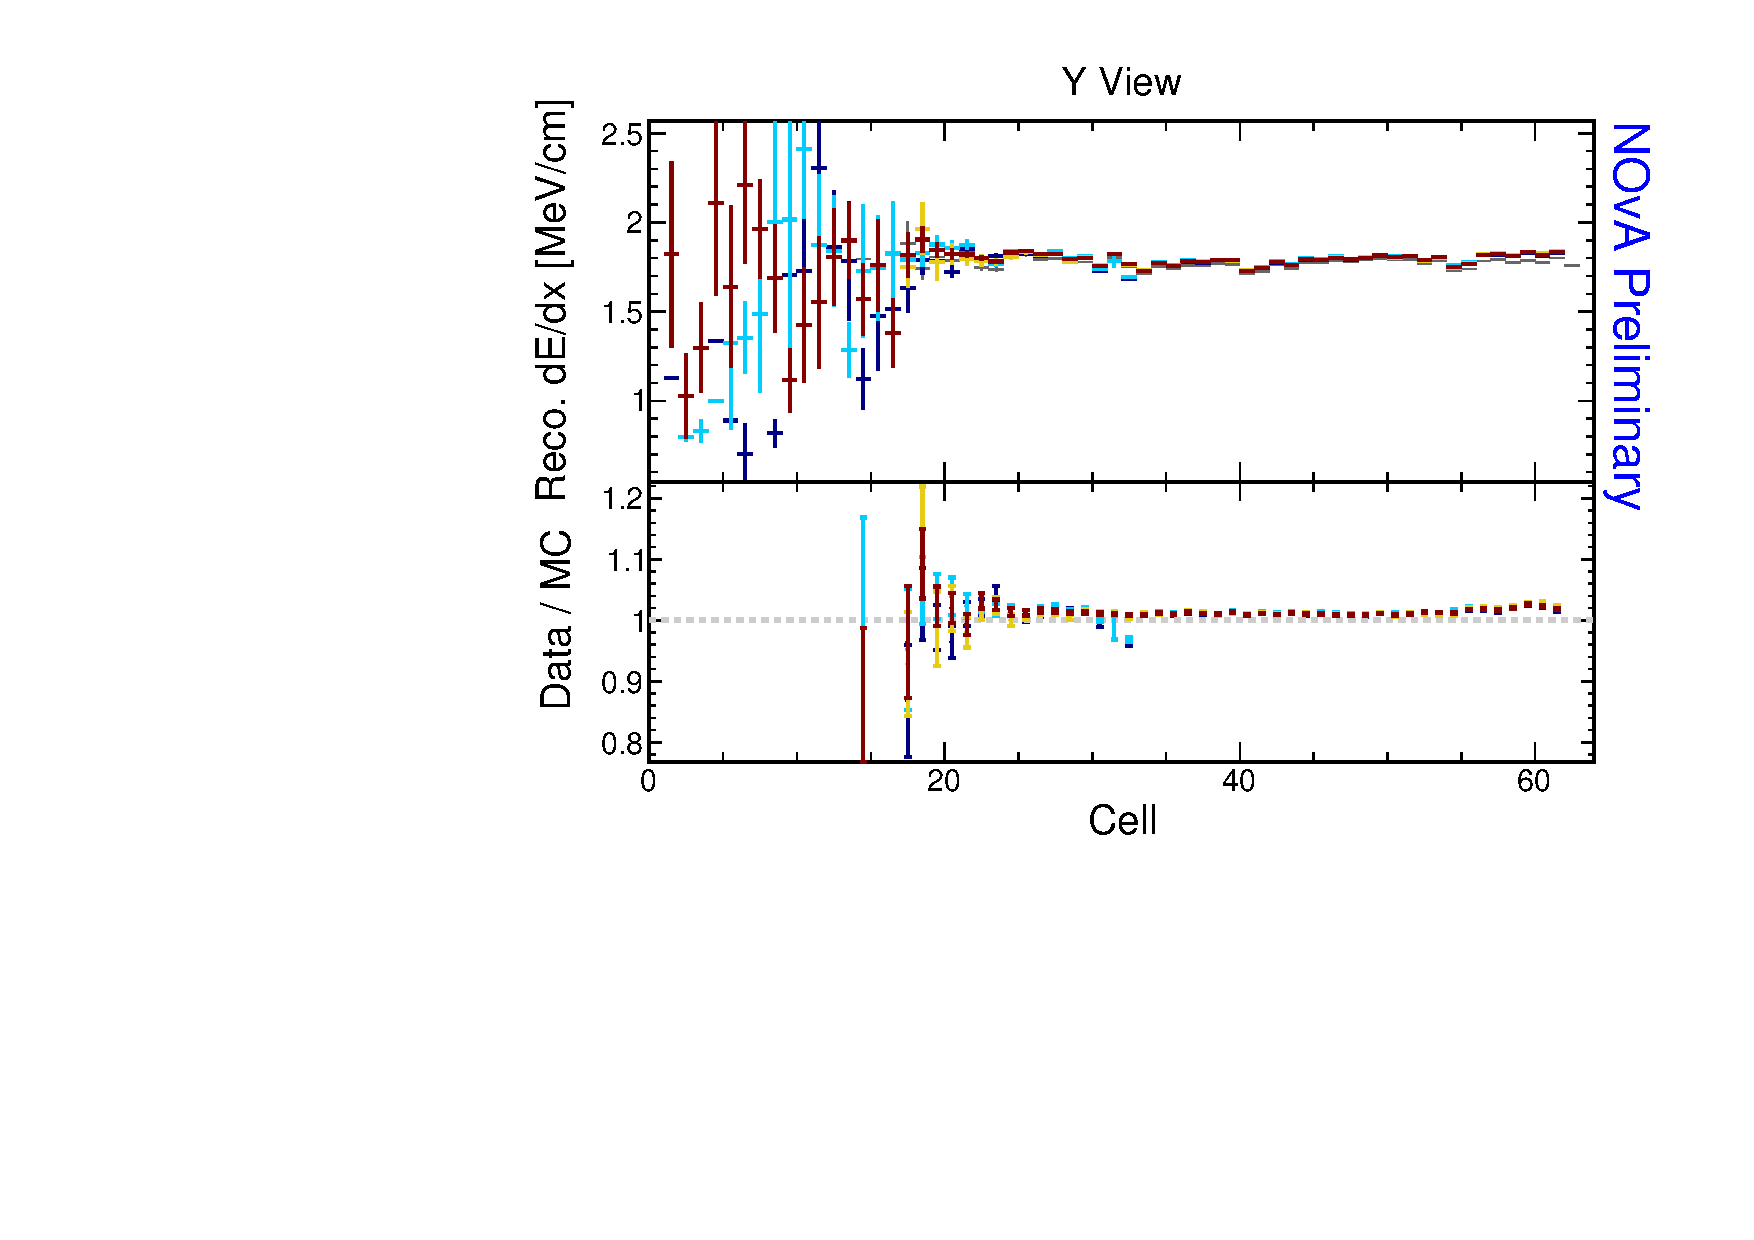
\includegraphics[width=\linewidth]{Plots/Calibana/recomevcm_cell_y.pdf}
  \end{subfigure}
  \caption{Distributions of stopping muons within a 1-2 m track window from the end of their tracks across the cells of the detector.}
  %\label{fig:AbsCalibCell1}
\end{figure}

\begin{figure}[!ht]
  \begin{subfigure}{\textwidth}
  \centering
    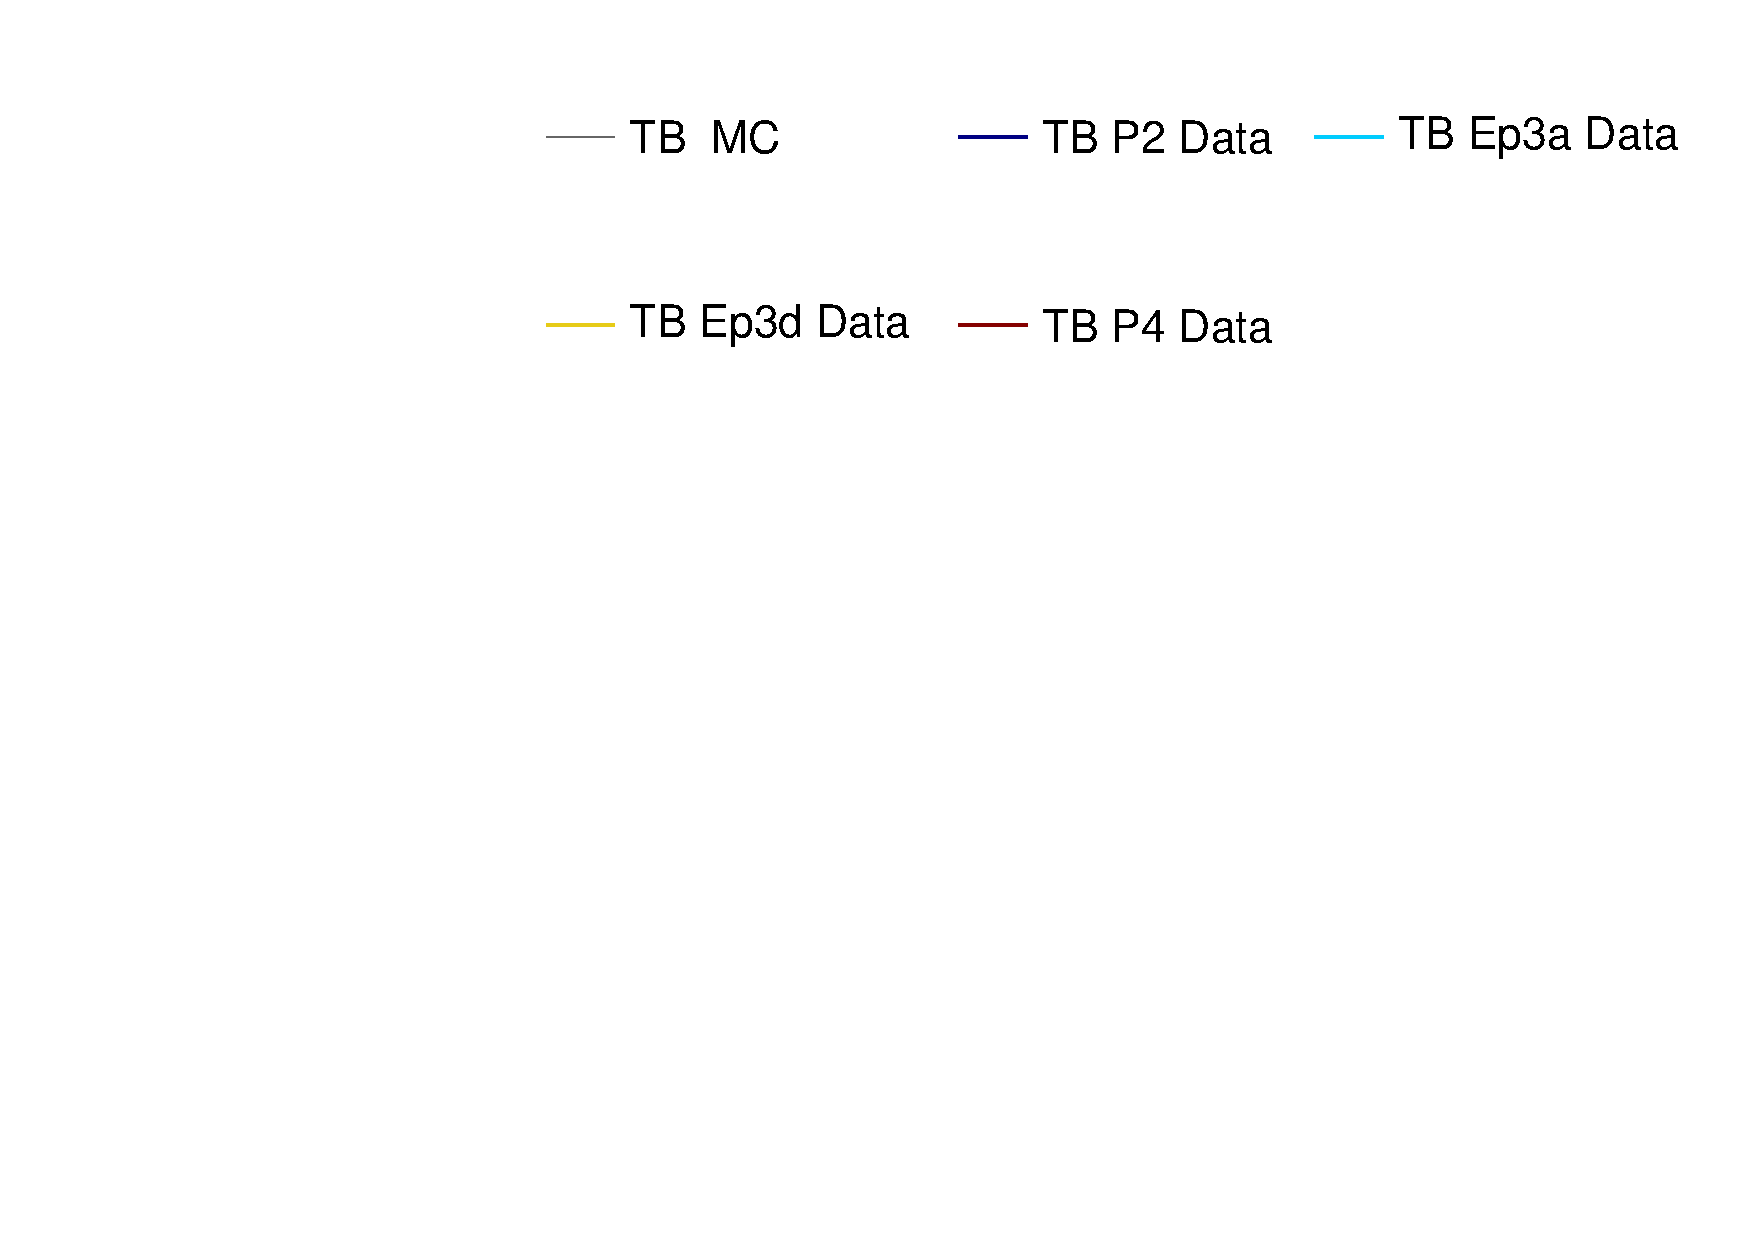
\includegraphics[height=0.2\linewidth]{Plots/Calibana/legend.pdf}
  \end{subfigure}
  \vspace*{2mm}

  \begin{subfigure}{0.495\textwidth}
    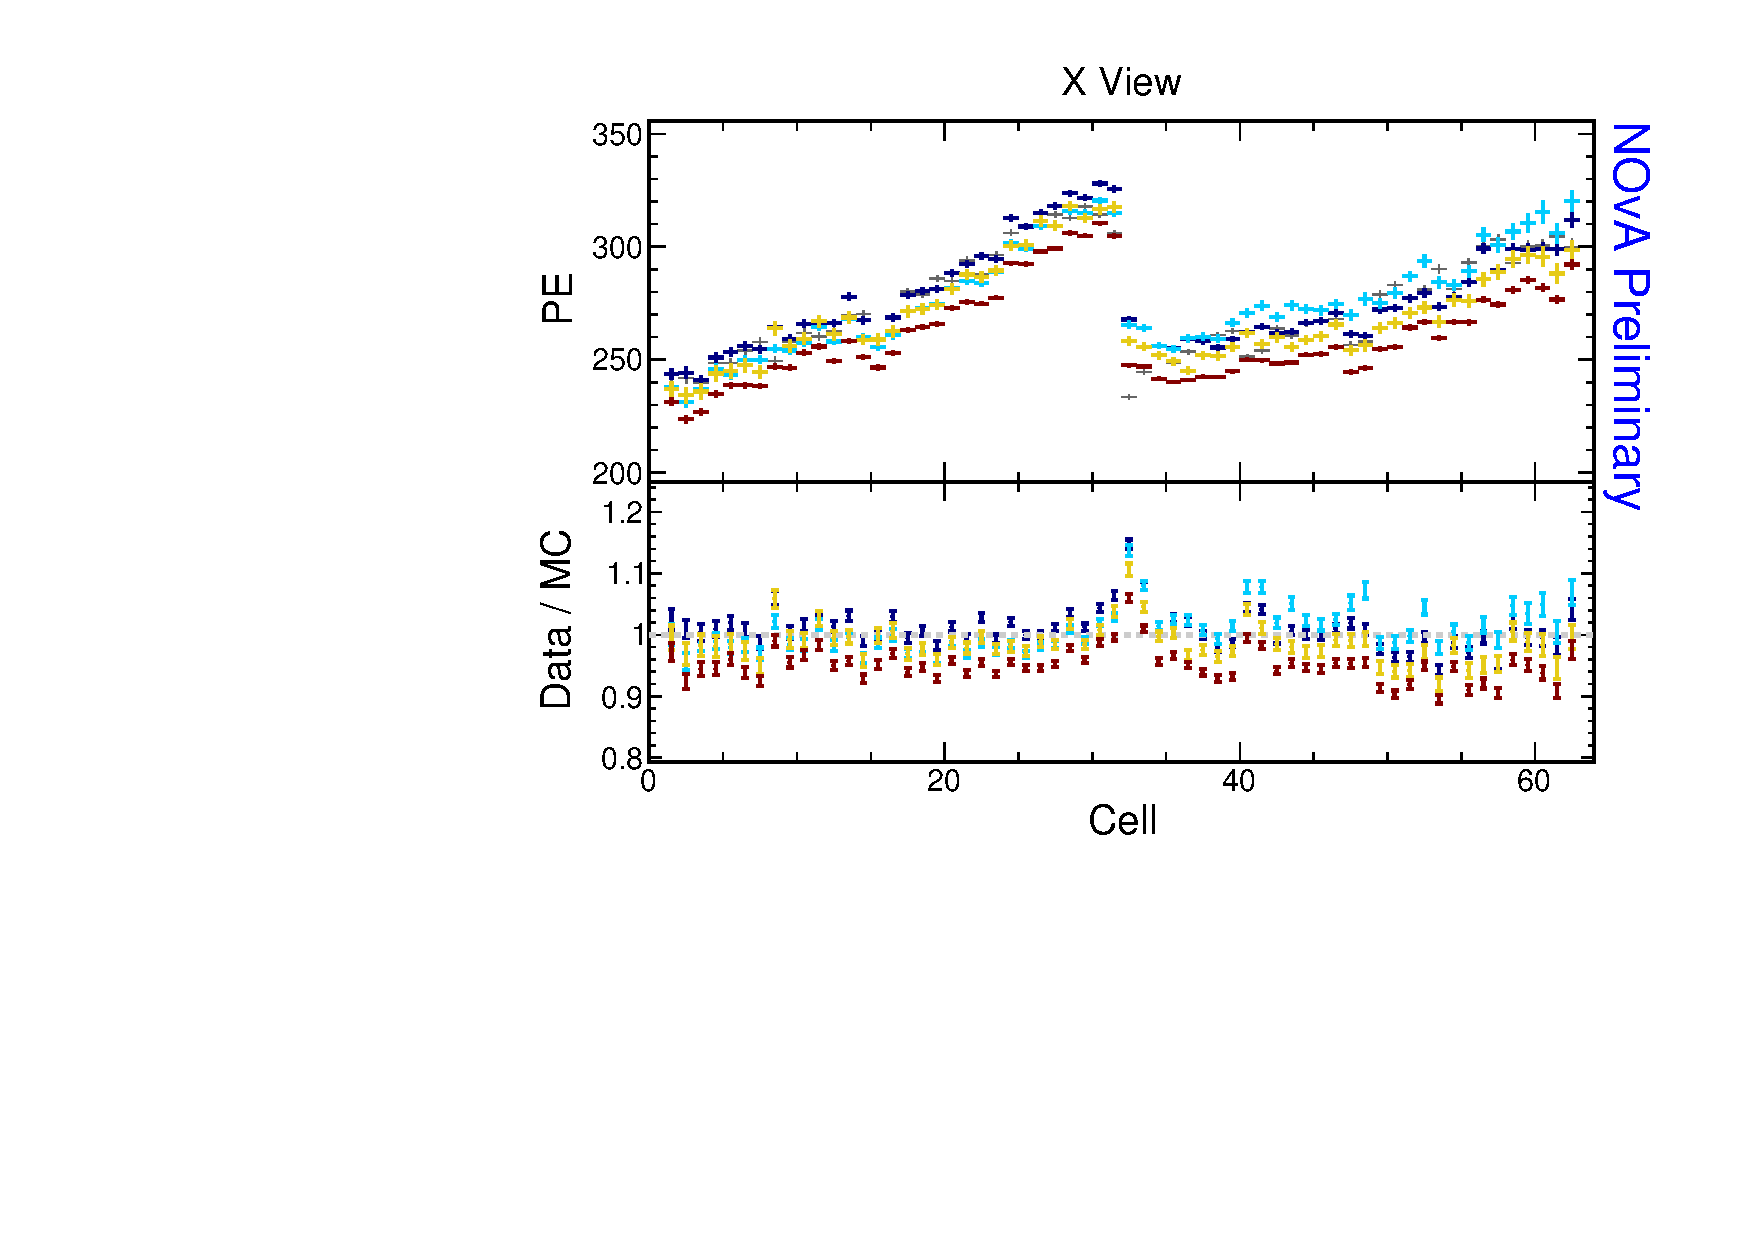
\includegraphics[width=\linewidth]{Plots/Calibana/pe_cell_x.pdf}
  \end{subfigure}
  \begin{subfigure}{0.495\textwidth}
    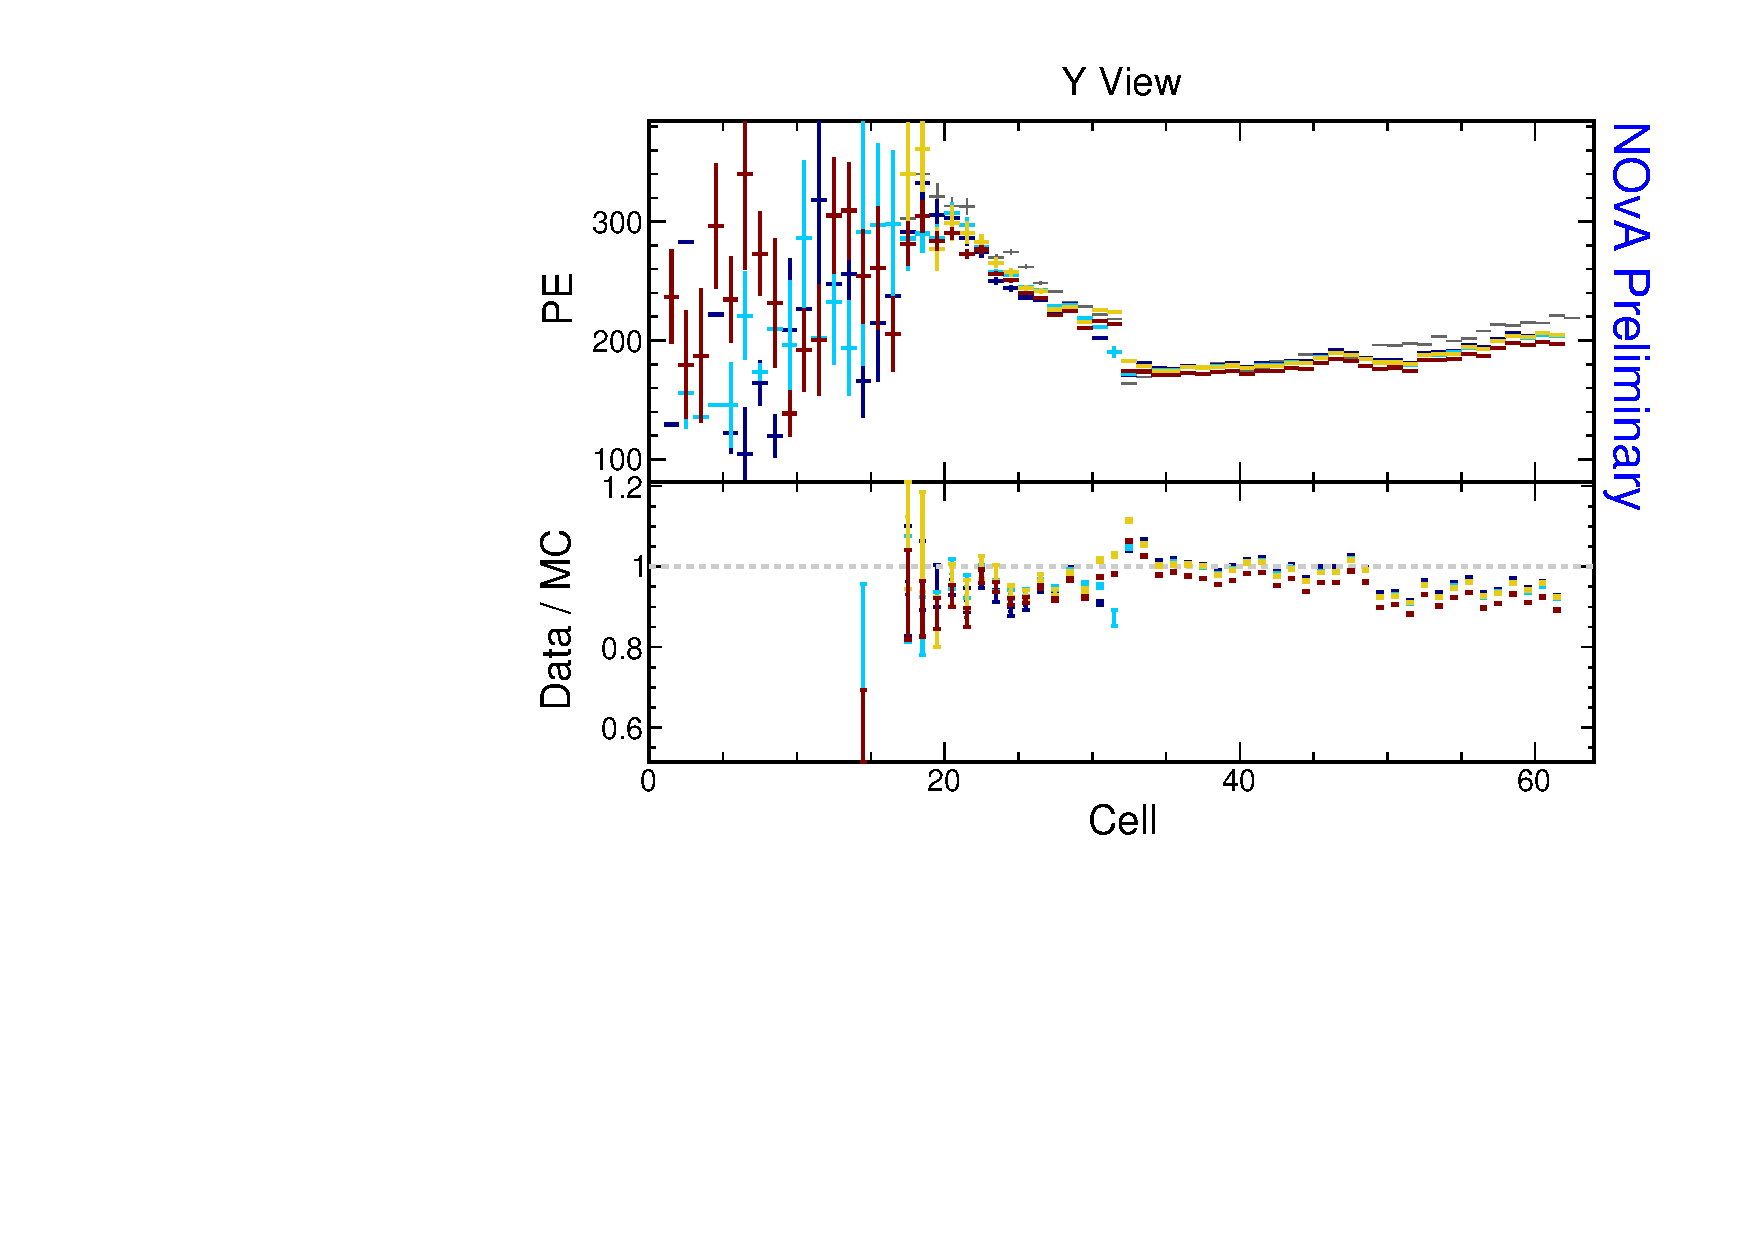
\includegraphics[width=\linewidth]{Plots/Calibana/pe_cell_y.pdf}
  \end{subfigure}
  \begin{subfigure}{0.495\textwidth}
    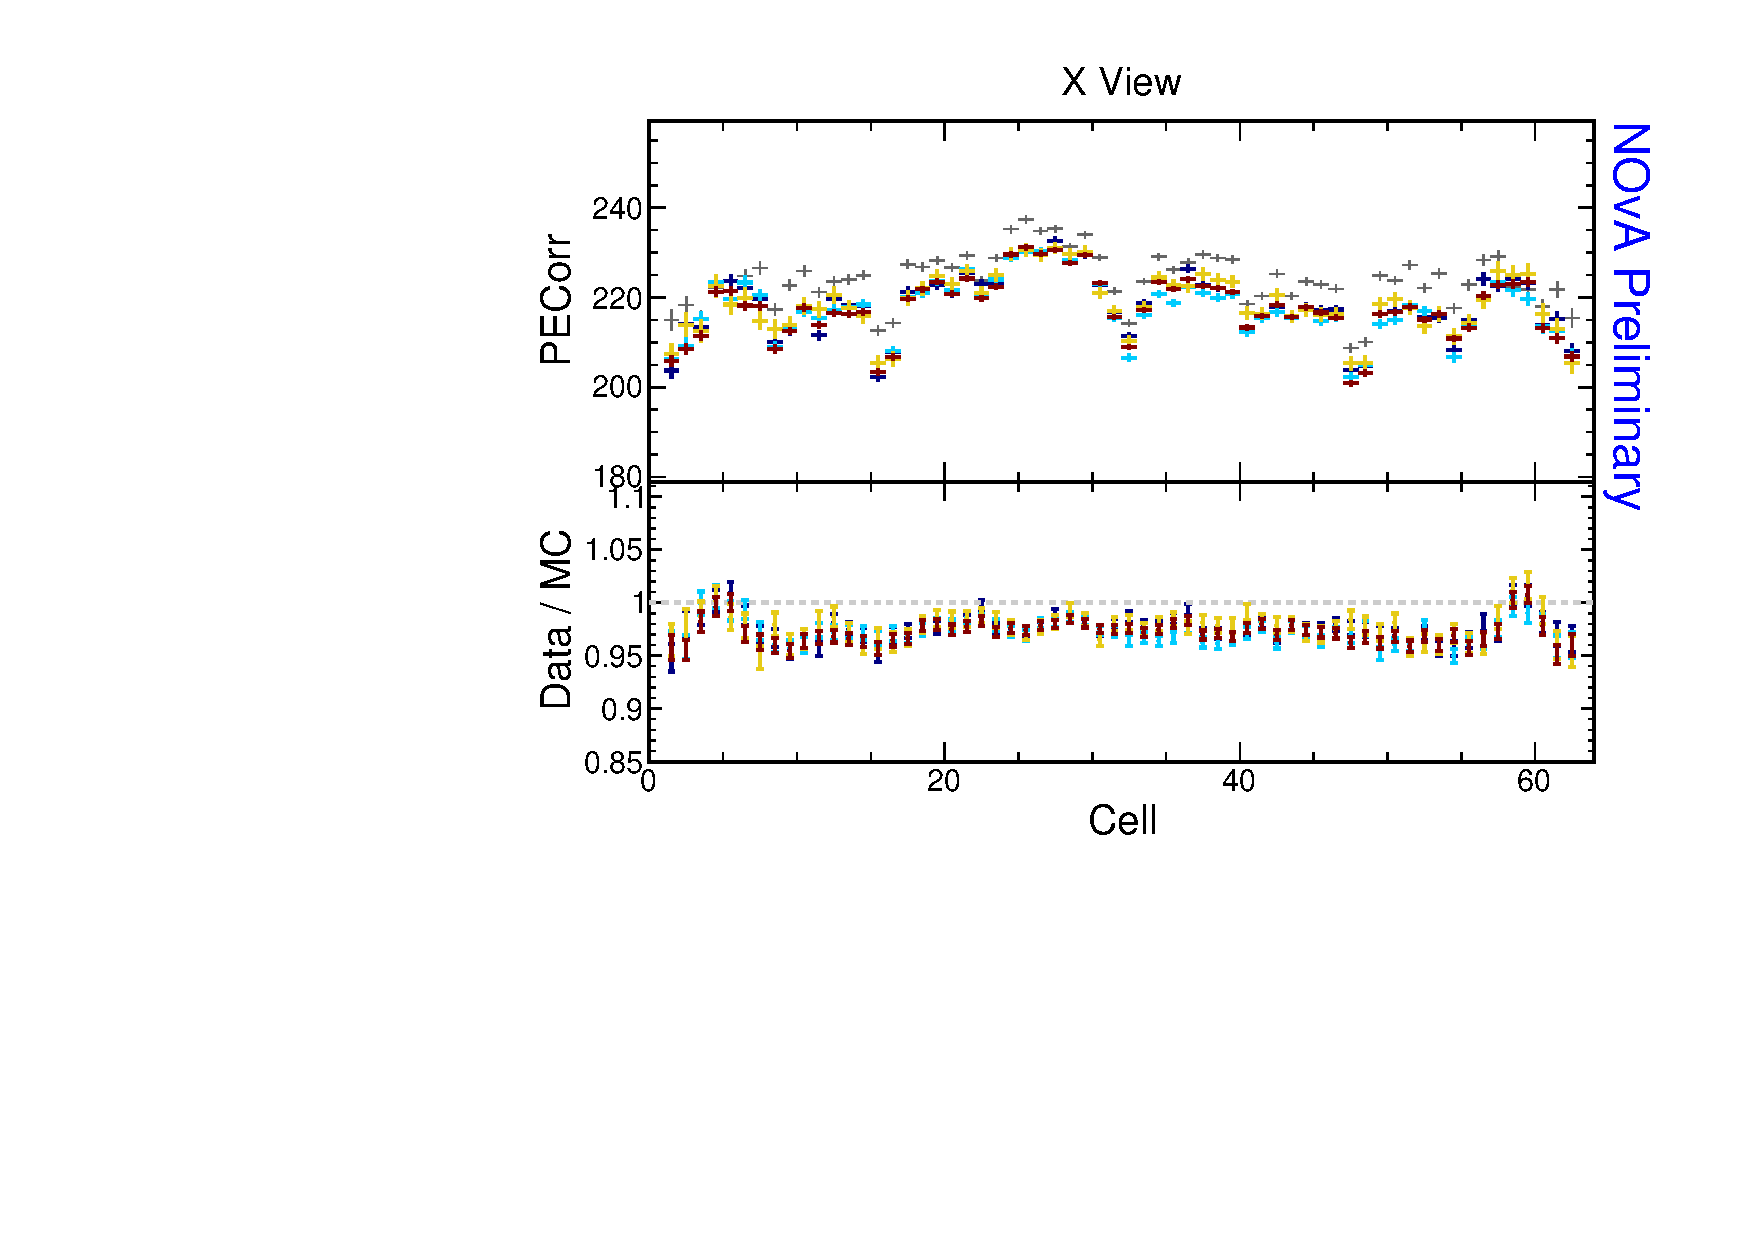
\includegraphics[width=\linewidth]{Plots/Calibana/pecorr_cell_x.pdf}
  \end{subfigure}
  \begin{subfigure}{0.495\textwidth}
    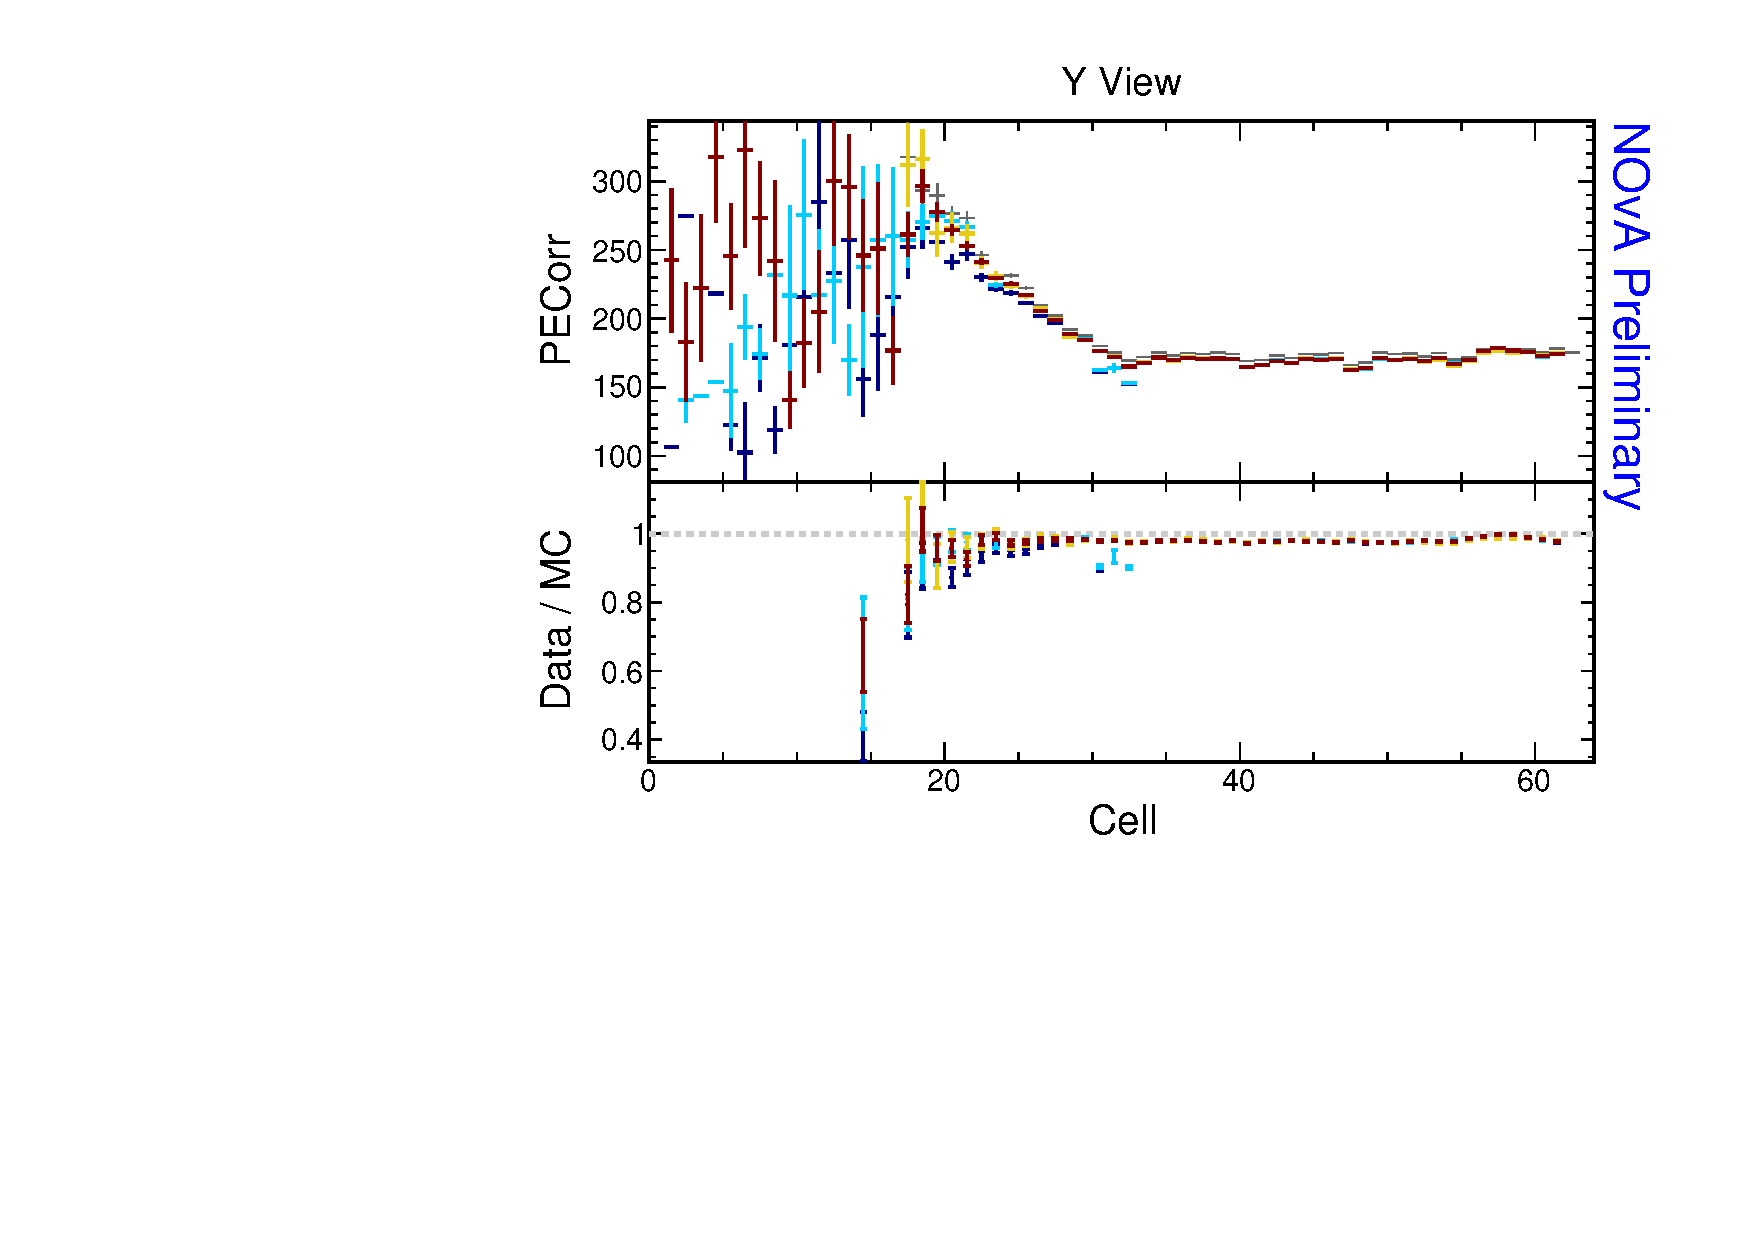
\includegraphics[width=\linewidth]{Plots/Calibana/pecorr_cell_y.pdf}
  \end{subfigure}
  \begin{subfigure}{0.495\textwidth}
    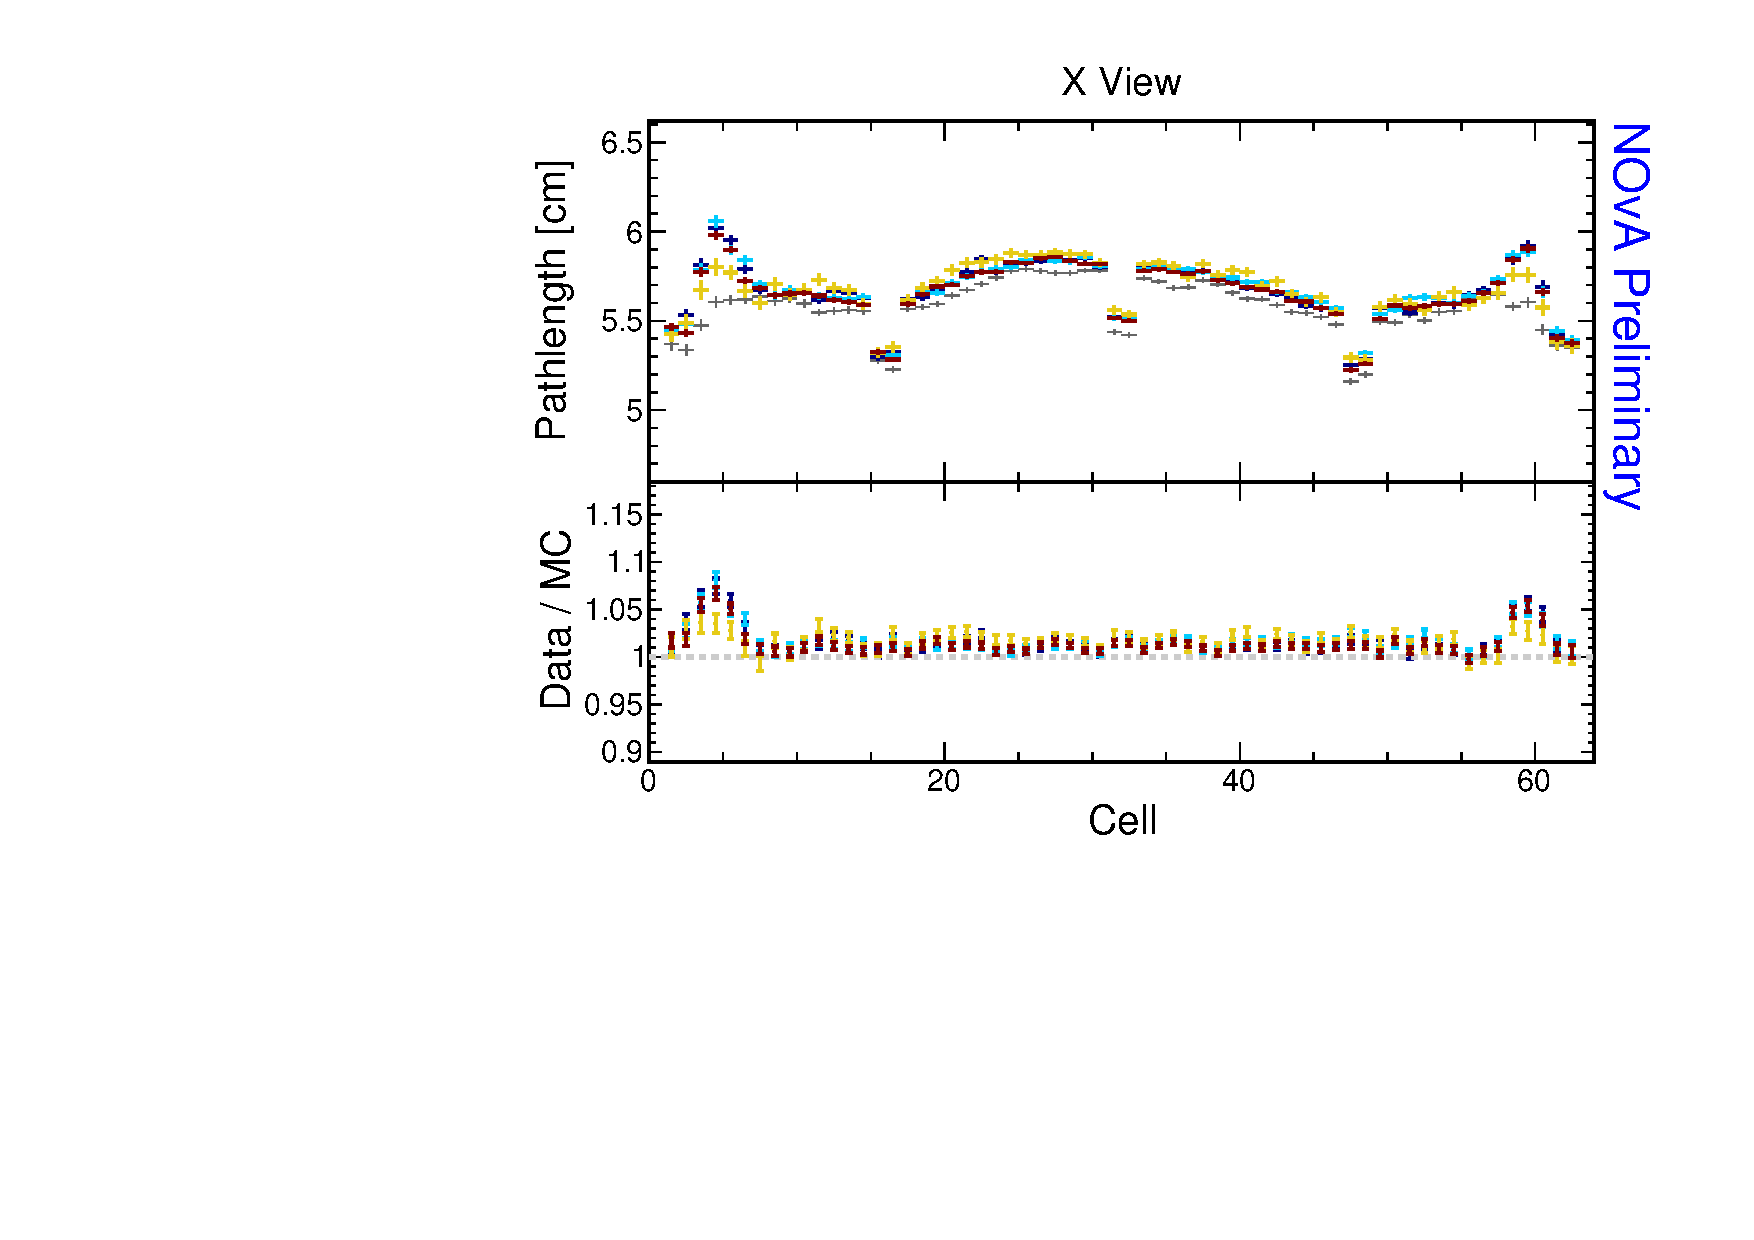
\includegraphics[width=\linewidth]{Plots/Calibana/cm_cell_x.pdf}
  \end{subfigure}
  \begin{subfigure}{0.495\textwidth}
    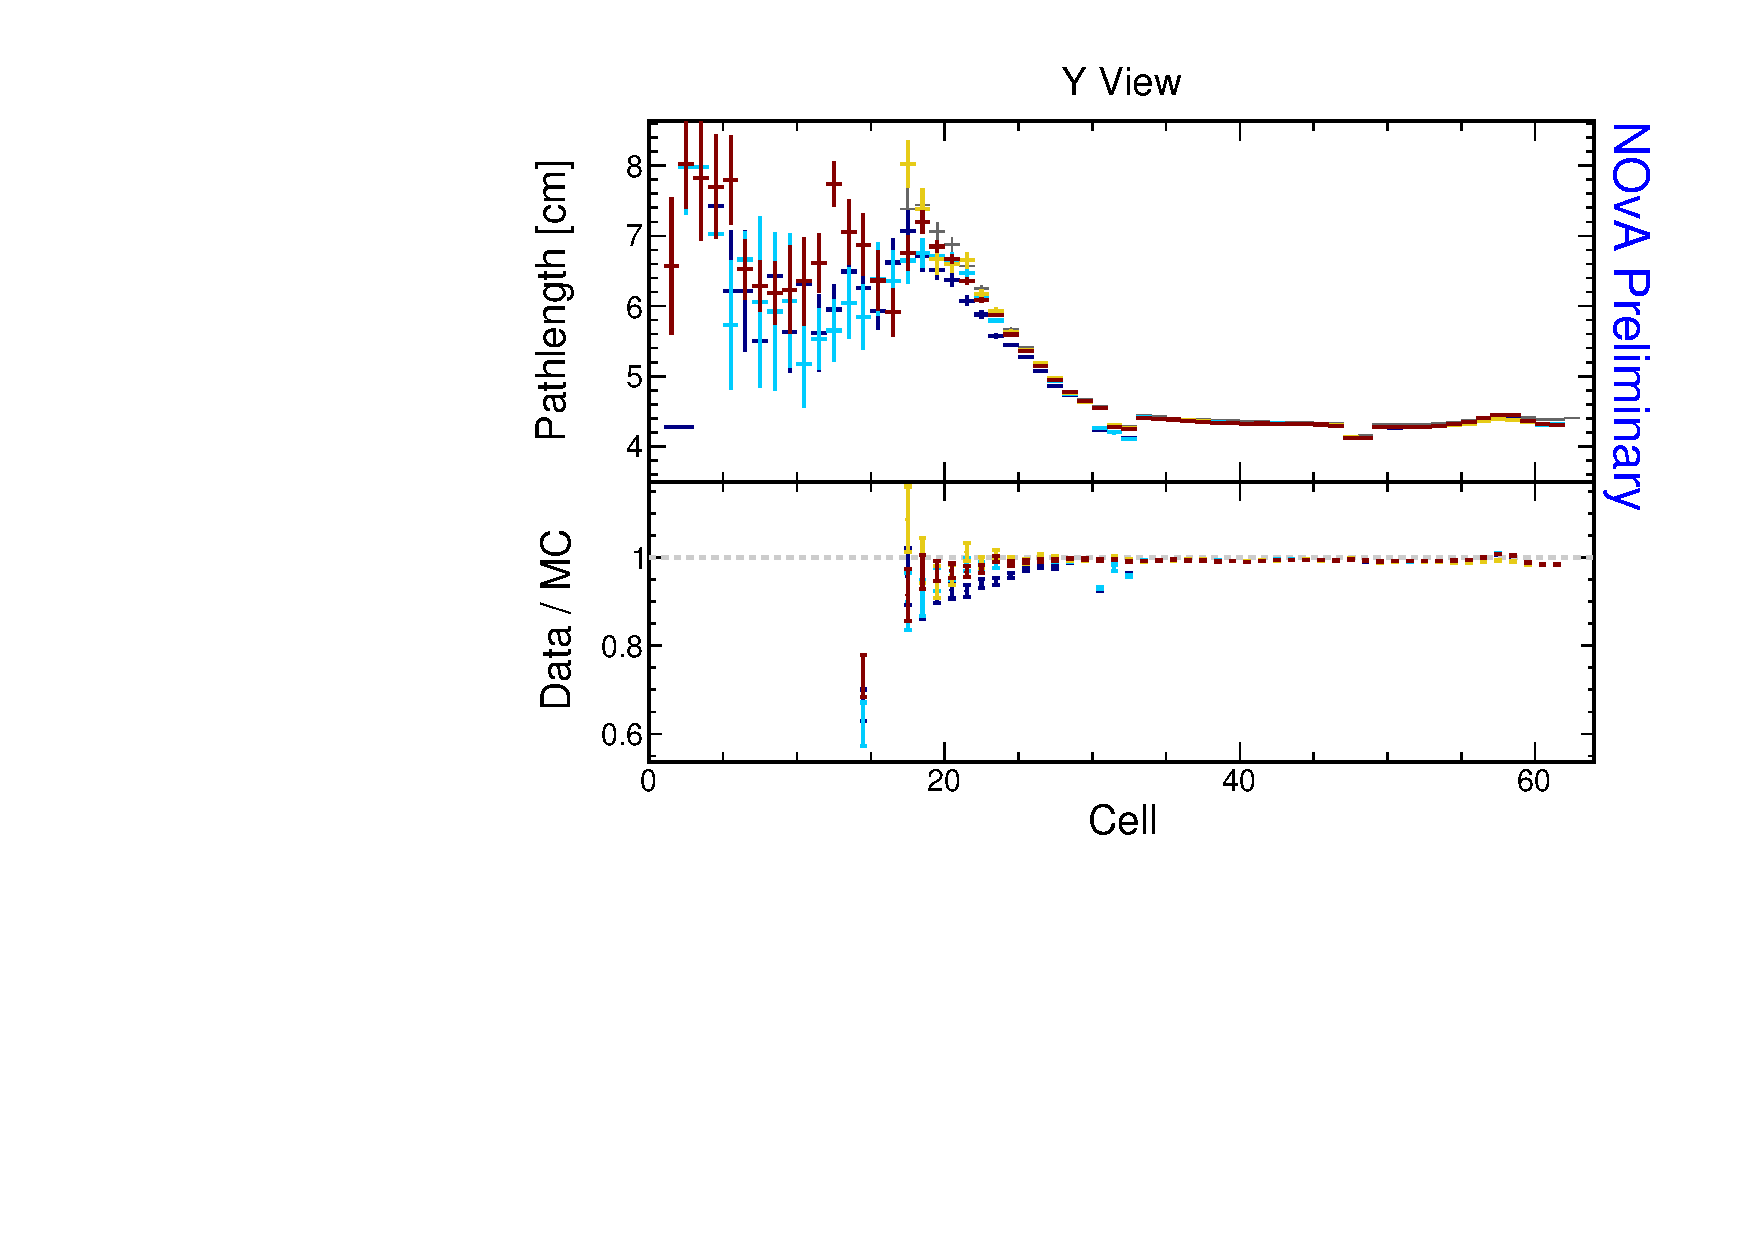
\includegraphics[width=\linewidth]{Plots/Calibana/cm_cell_y.pdf}
  \end{subfigure}
  \caption{Distributions of stopping muons within a 1-2 m track window from the end of their tracks across the cells of the detector.}
  %\label{fig:AbsCalibCell2}
\end{figure}

\begin{figure}[!ht]
  \begin{subfigure}{\textwidth}
  \centering
    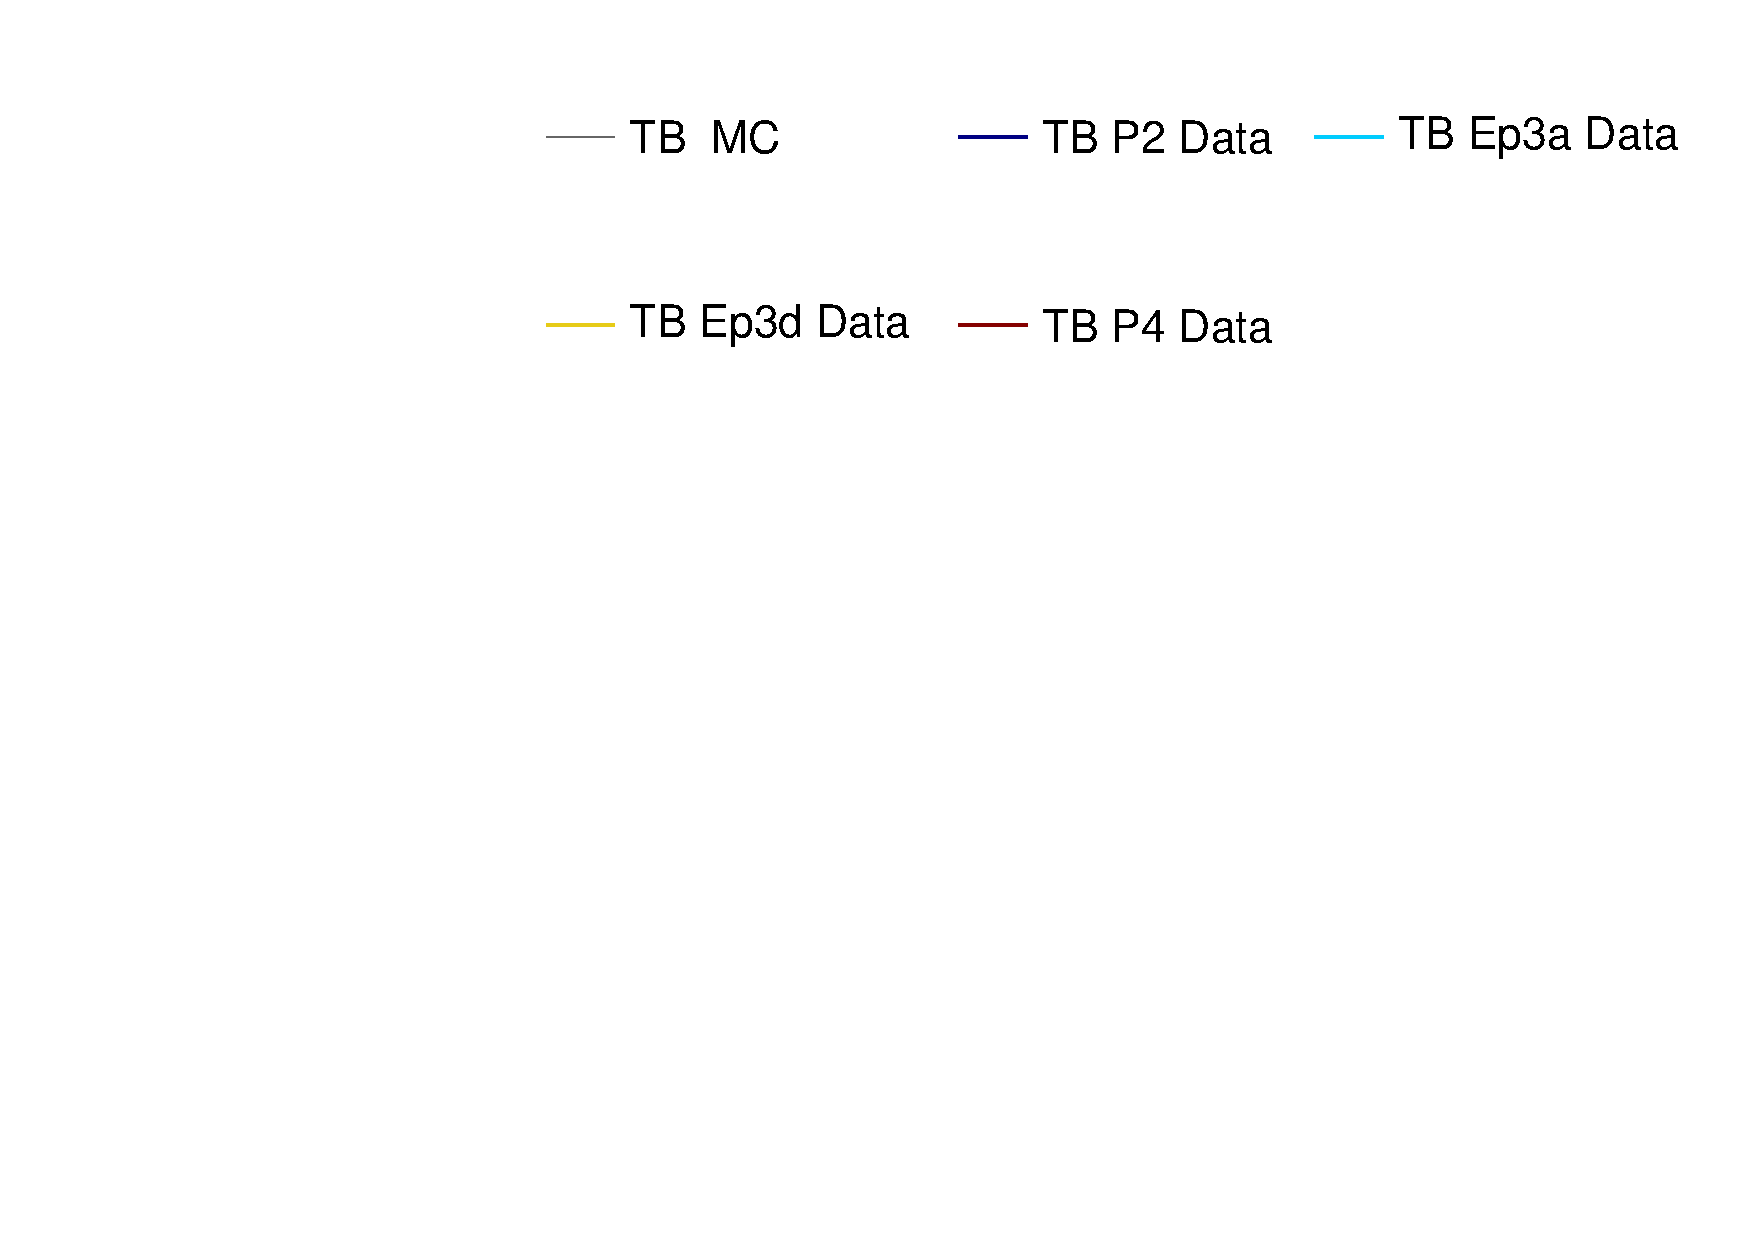
\includegraphics[height=0.2\linewidth]{Plots/Calibana/legend.pdf}
  \end{subfigure}
  \vspace*{2mm}

  \begin{subfigure}{0.495\textwidth}
    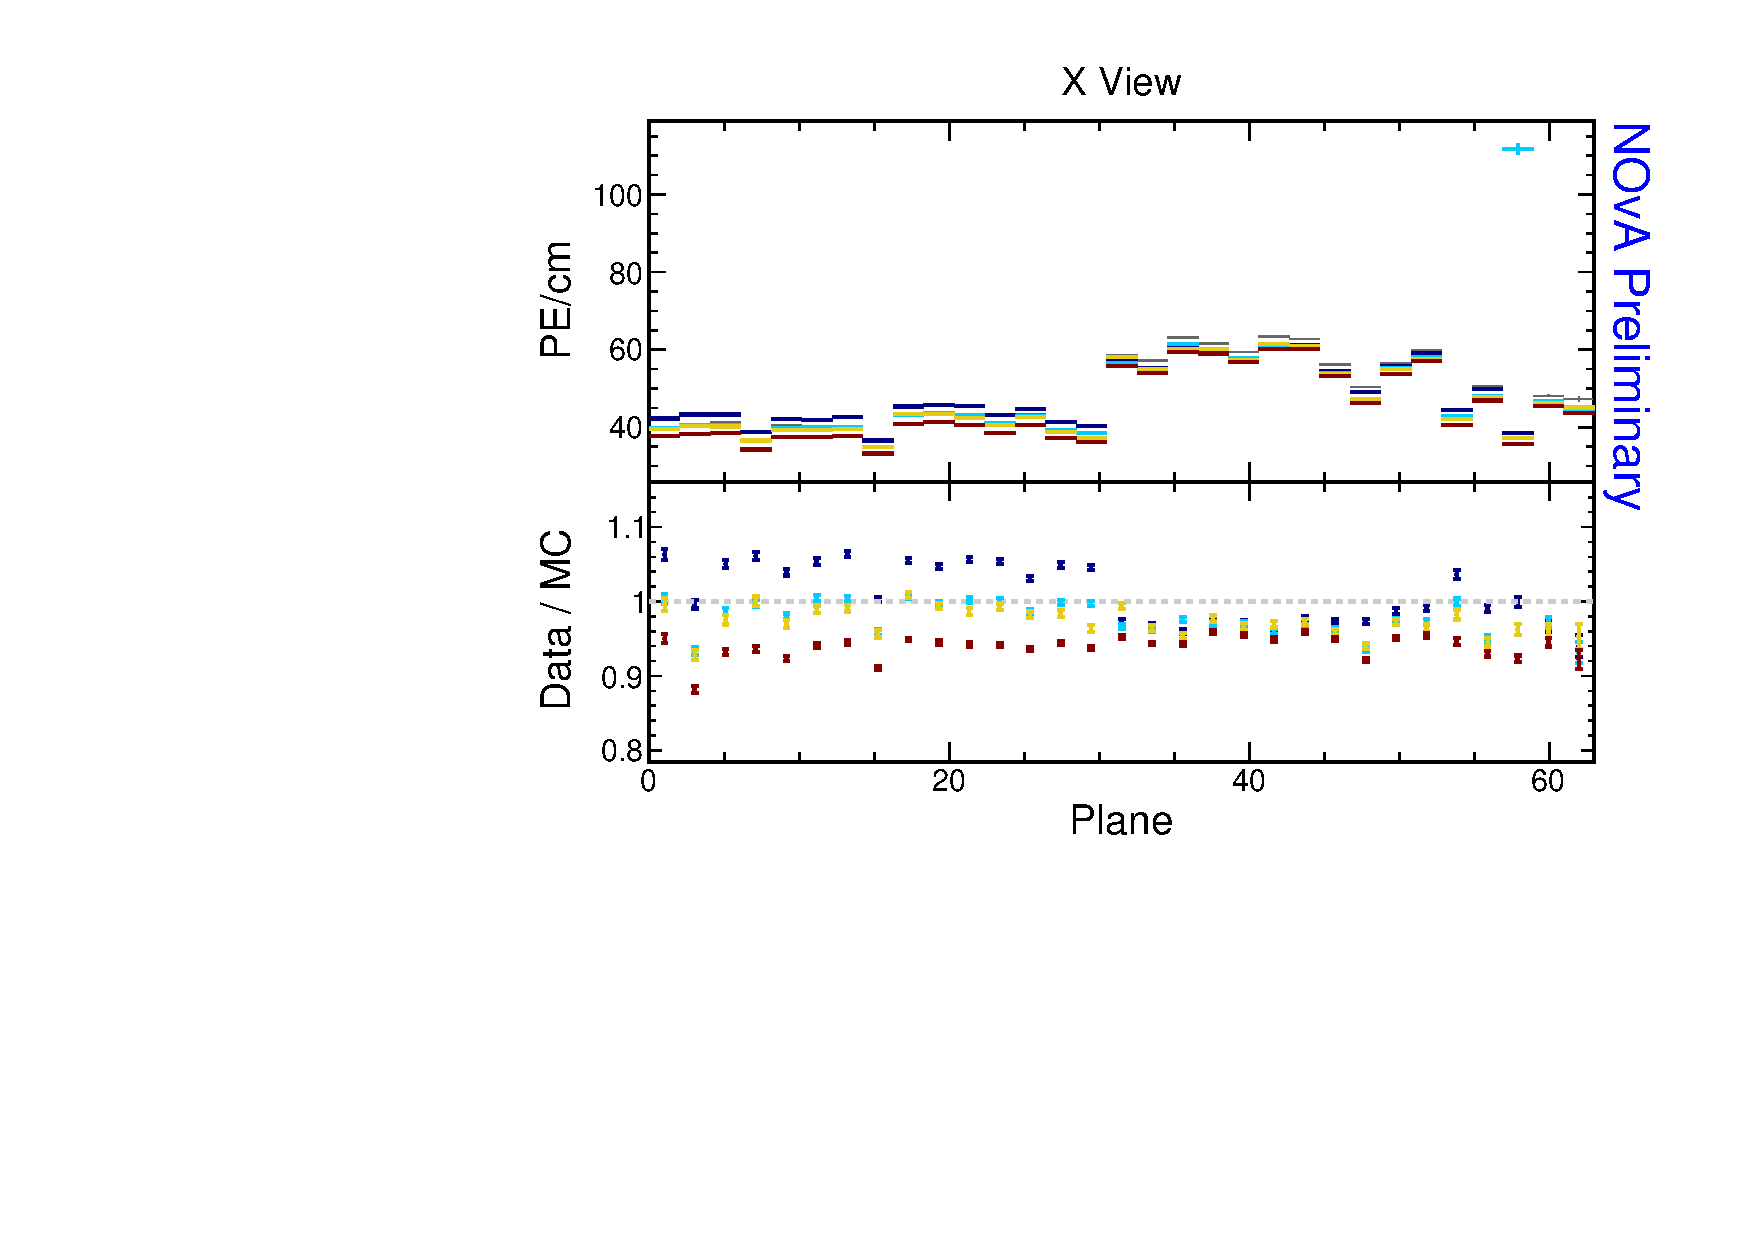
\includegraphics[width=\linewidth]{Plots/Calibana/pecm_plane_x.pdf}
  \end{subfigure}
  \begin{subfigure}{0.495\textwidth}
    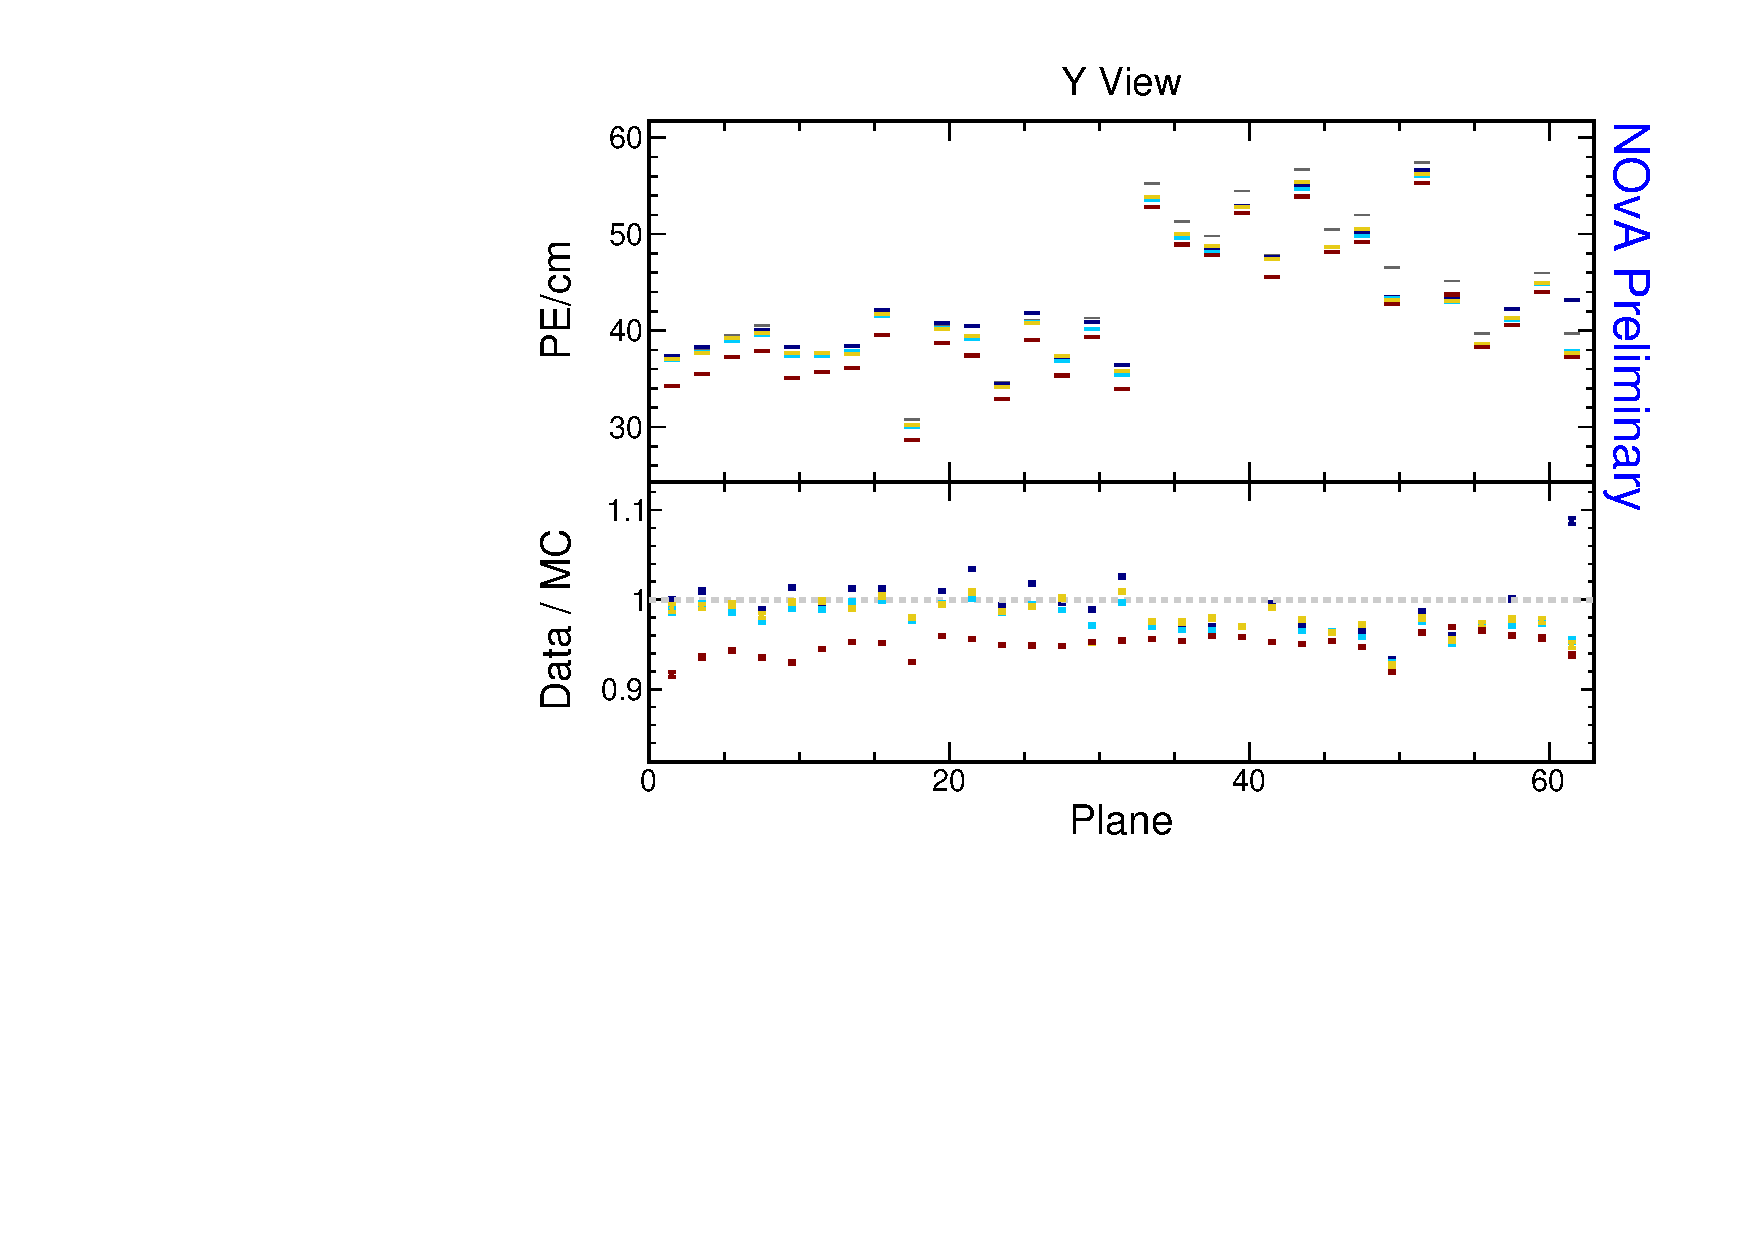
\includegraphics[width=\linewidth]{Plots/Calibana/pecm_plane_y.pdf}
  \end{subfigure}
  \begin{subfigure}{0.495\textwidth}
    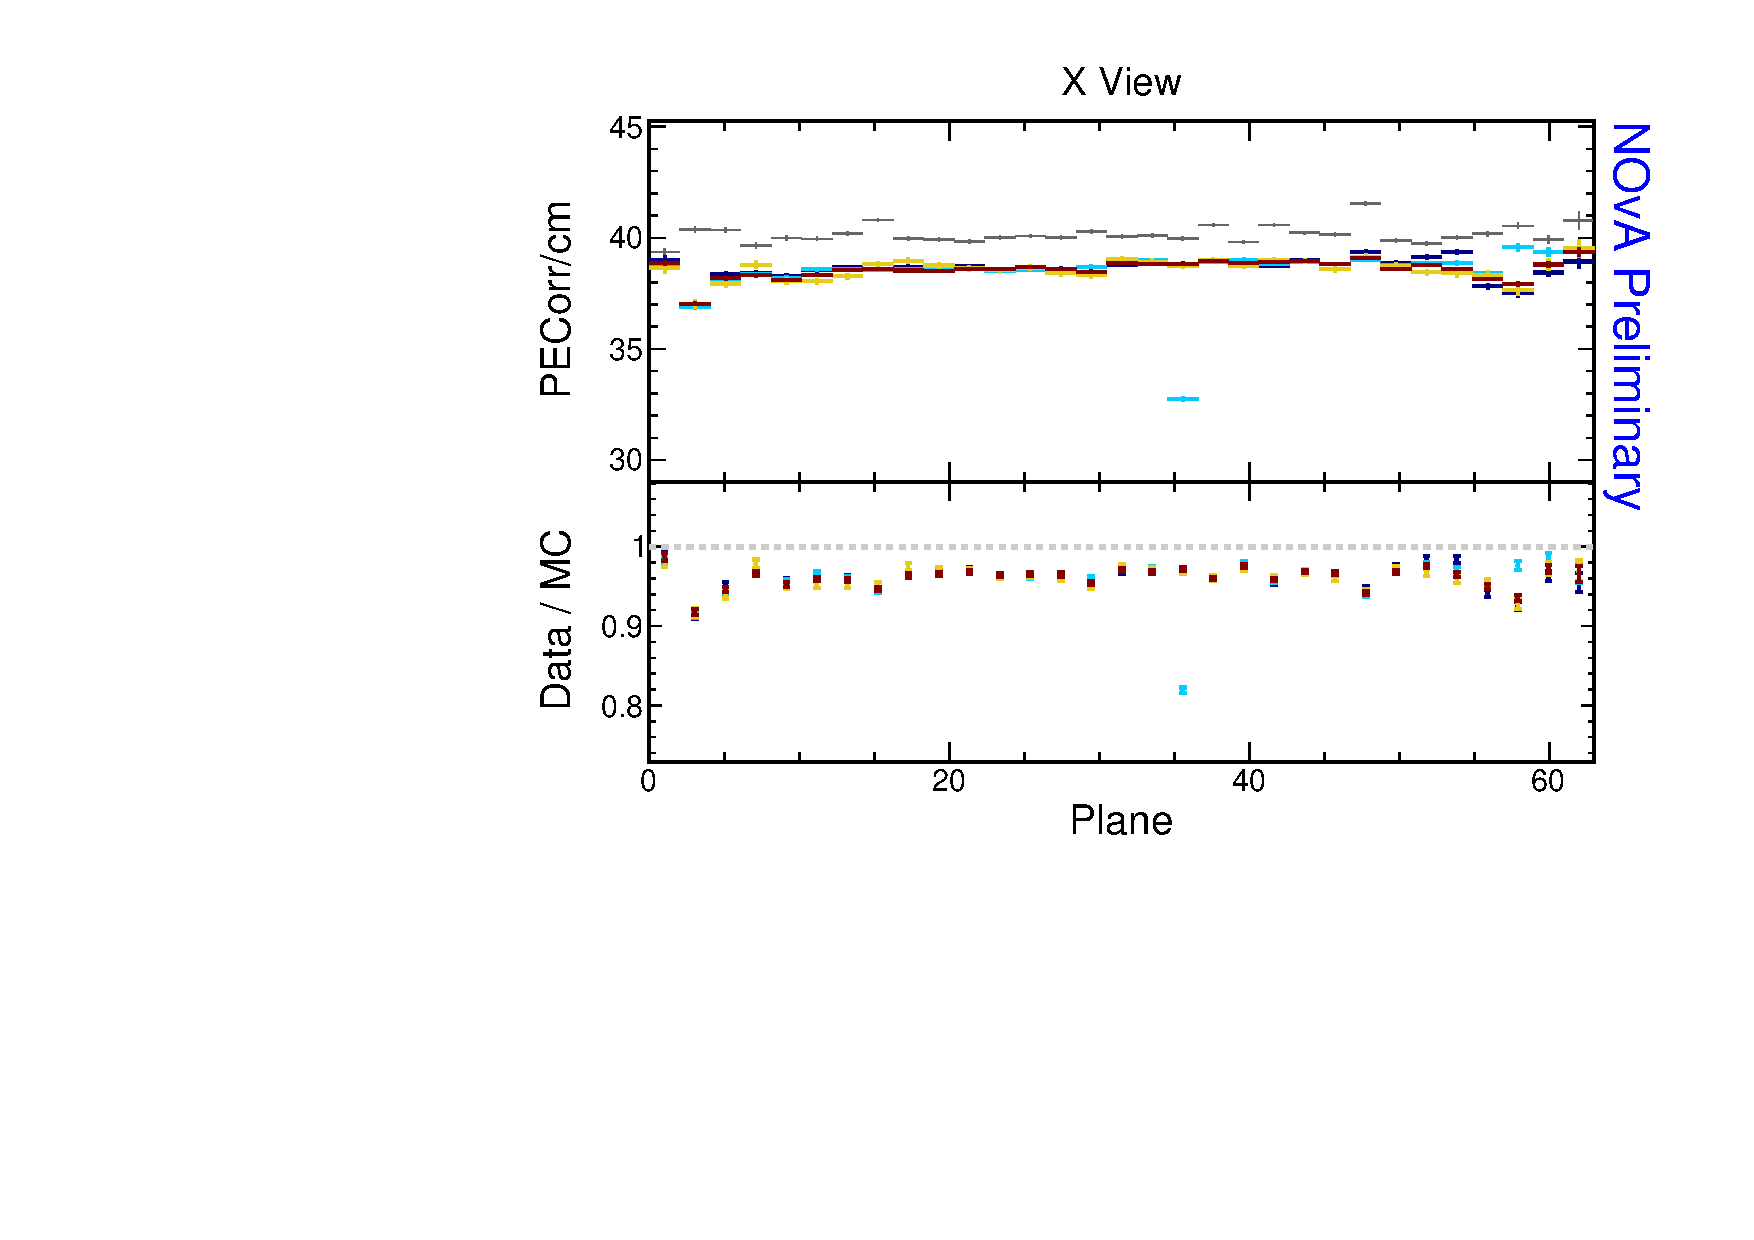
\includegraphics[width=\linewidth]{Plots/Calibana/pecorrcm_plane_x.pdf}
  \end{subfigure}
  \begin{subfigure}{0.495\textwidth}
    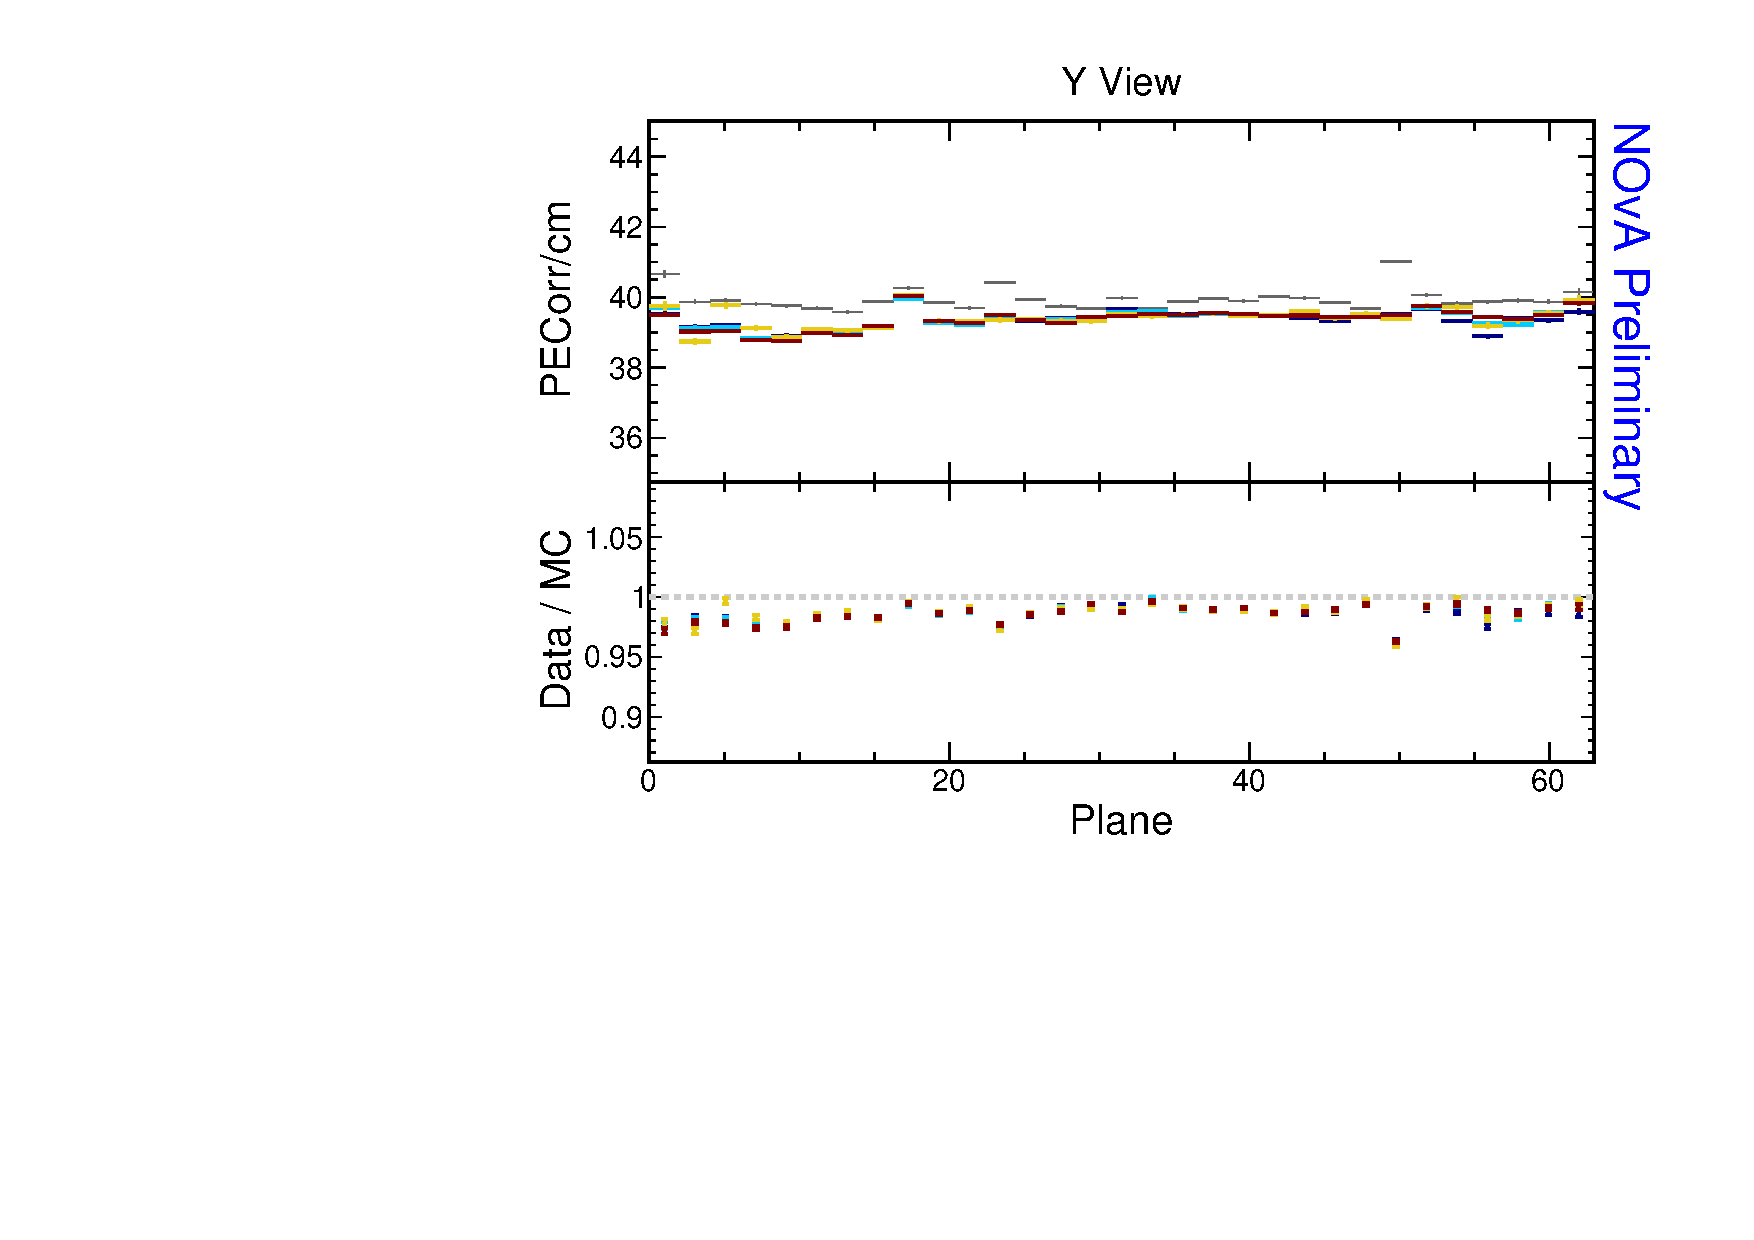
\includegraphics[width=\linewidth]{Plots/Calibana/pecorrcm_plane_y.pdf}
  \end{subfigure}
    \begin{subfigure}{0.495\textwidth}
    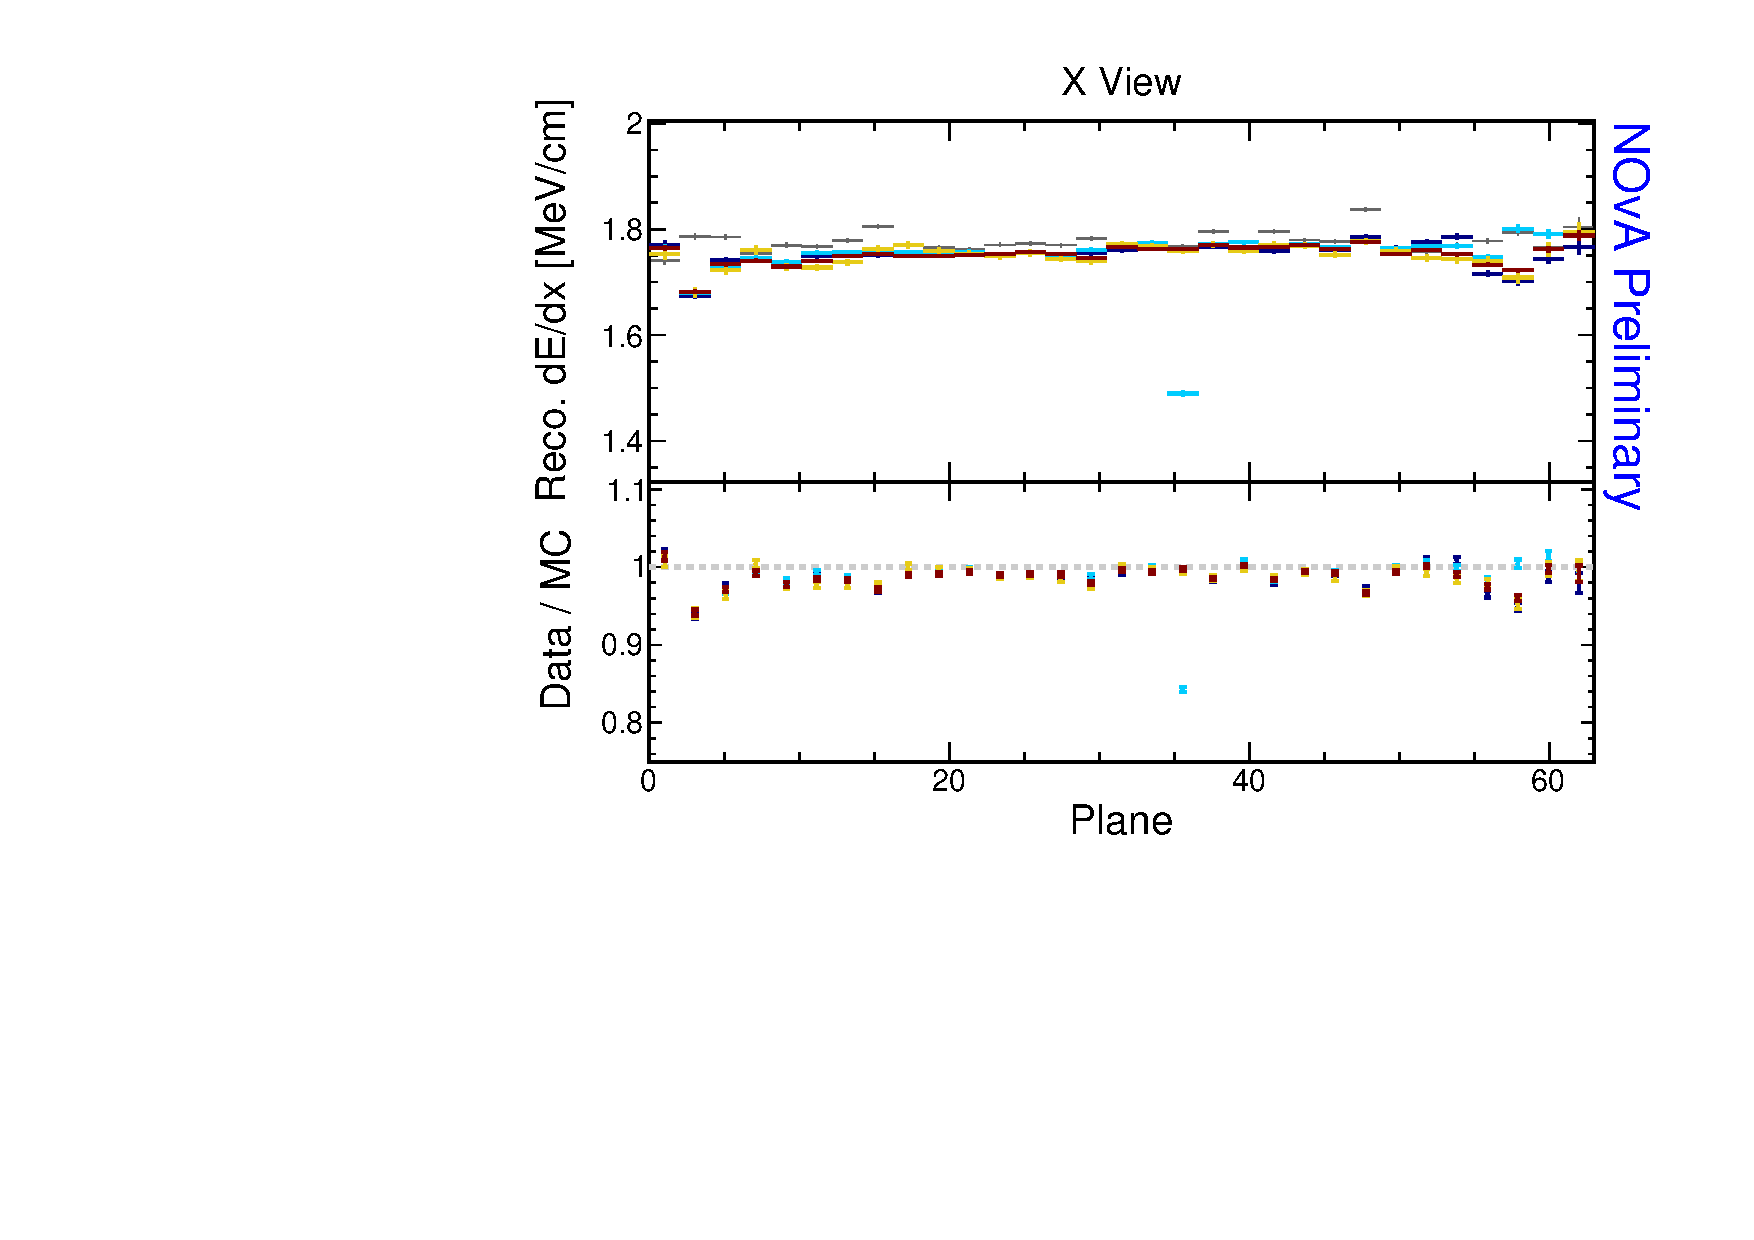
\includegraphics[width=\linewidth]{Plots/Calibana/recomevcm_plane_x.pdf}
  \end{subfigure}
  \begin{subfigure}{0.495\textwidth}
    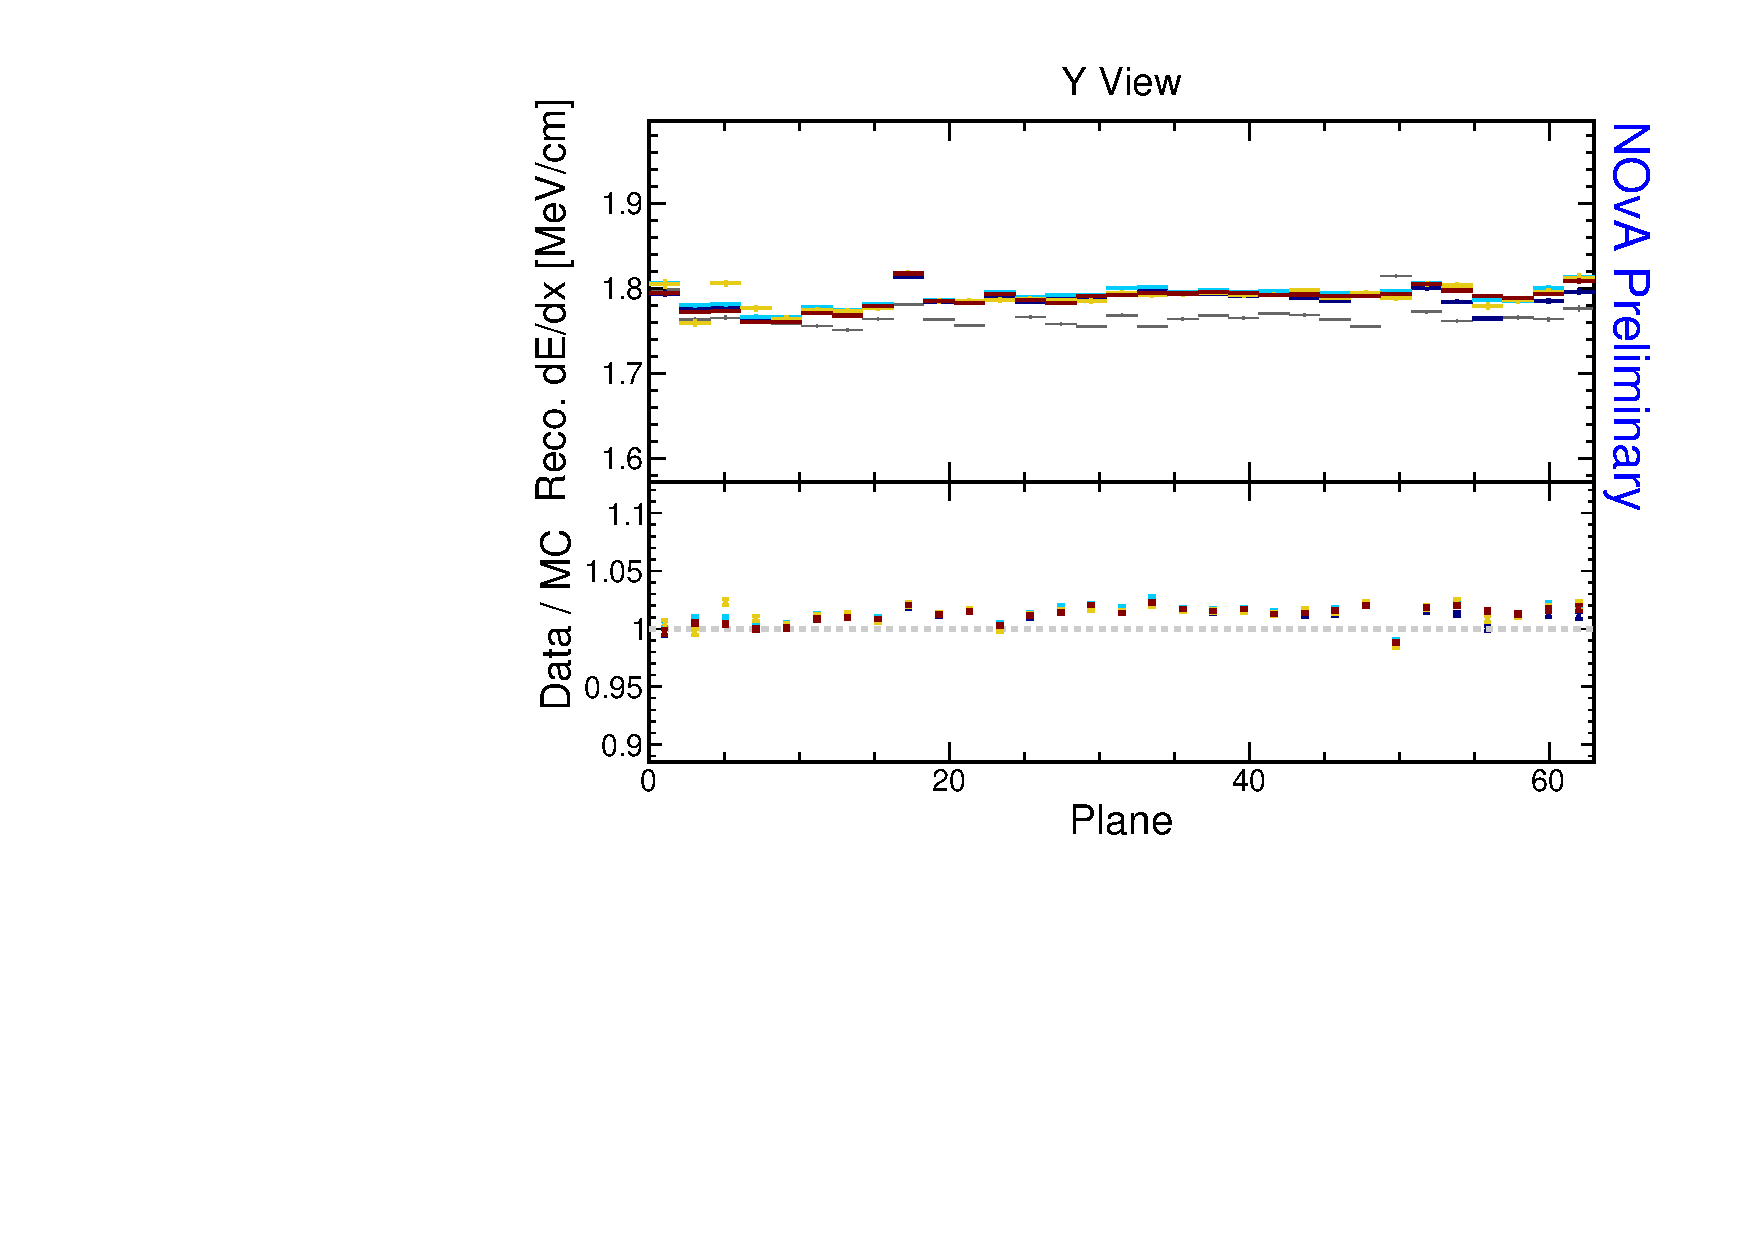
\includegraphics[width=\linewidth]{Plots/Calibana/recomevcm_plane_y.pdf}
  \end{subfigure}
  \caption{Distributions of stopping muons within a 1-2 m track window from the end of their tracks across the planes of the detector.}
  %\label{fig:AbsCalibPlane1}
\end{figure}

\begin{figure}[!ht]
  \begin{subfigure}{\textwidth}
  \centering
    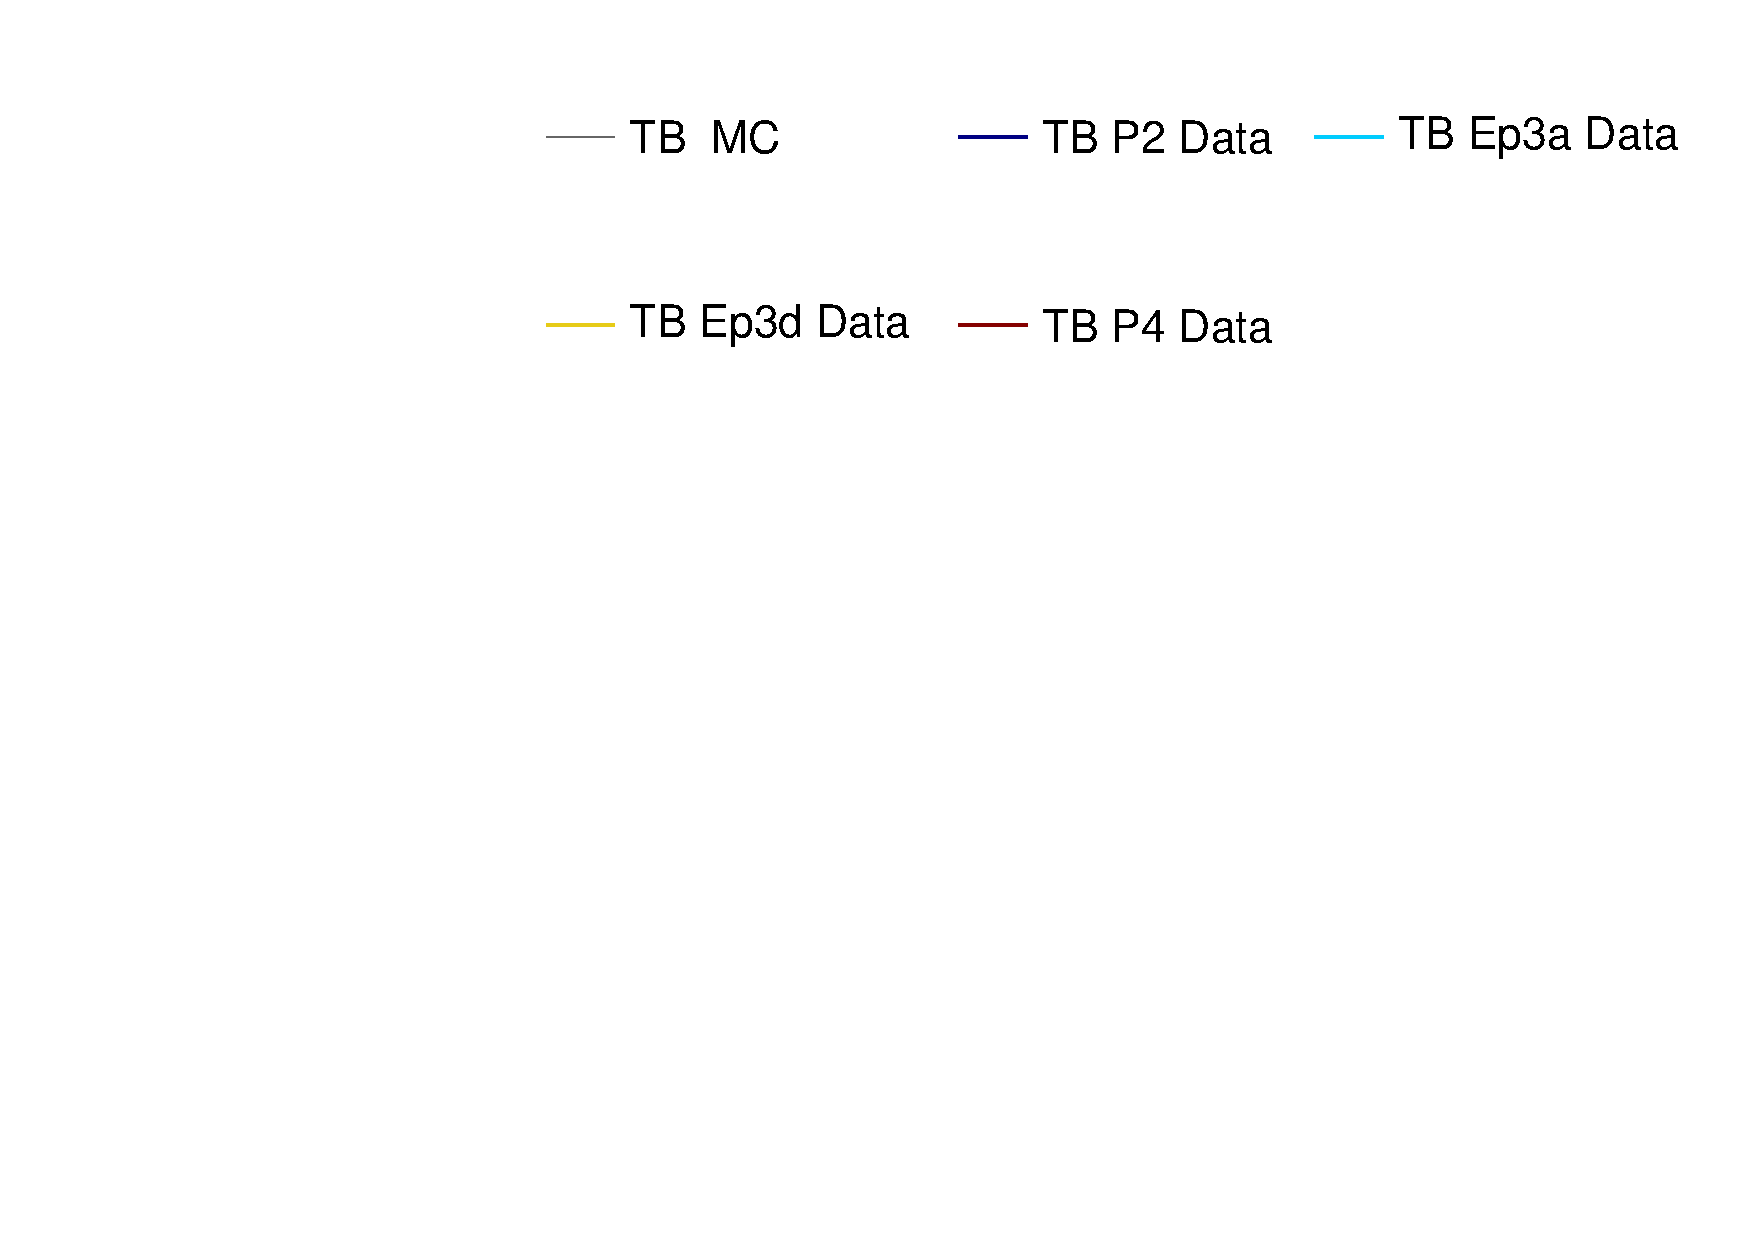
\includegraphics[height=0.2\linewidth]{Plots/Calibana/legend.pdf}
  \end{subfigure}
  \vspace*{2mm}

  \begin{subfigure}{0.495\textwidth}
    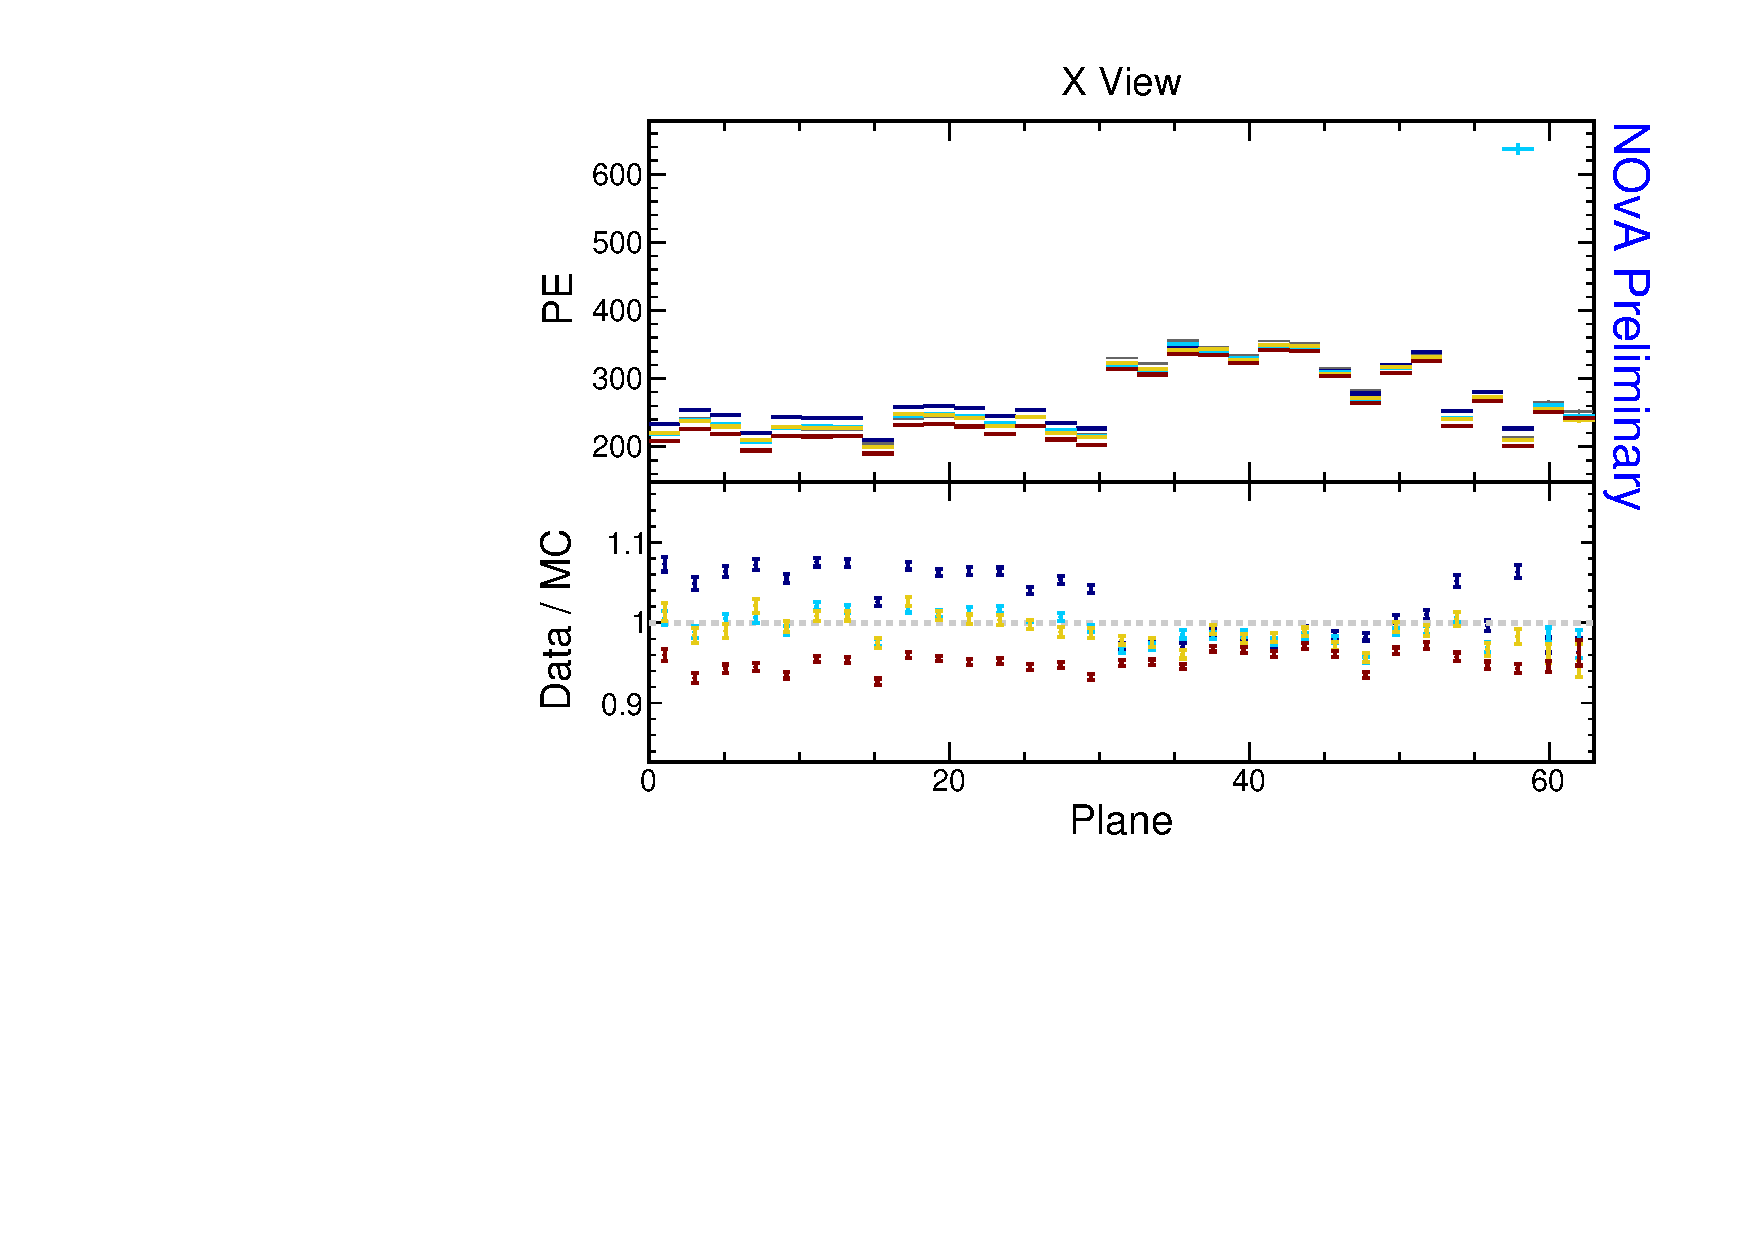
\includegraphics[width=\linewidth]{Plots/Calibana/pe_plane_x.pdf}
  \end{subfigure}
  \begin{subfigure}{0.495\textwidth}
    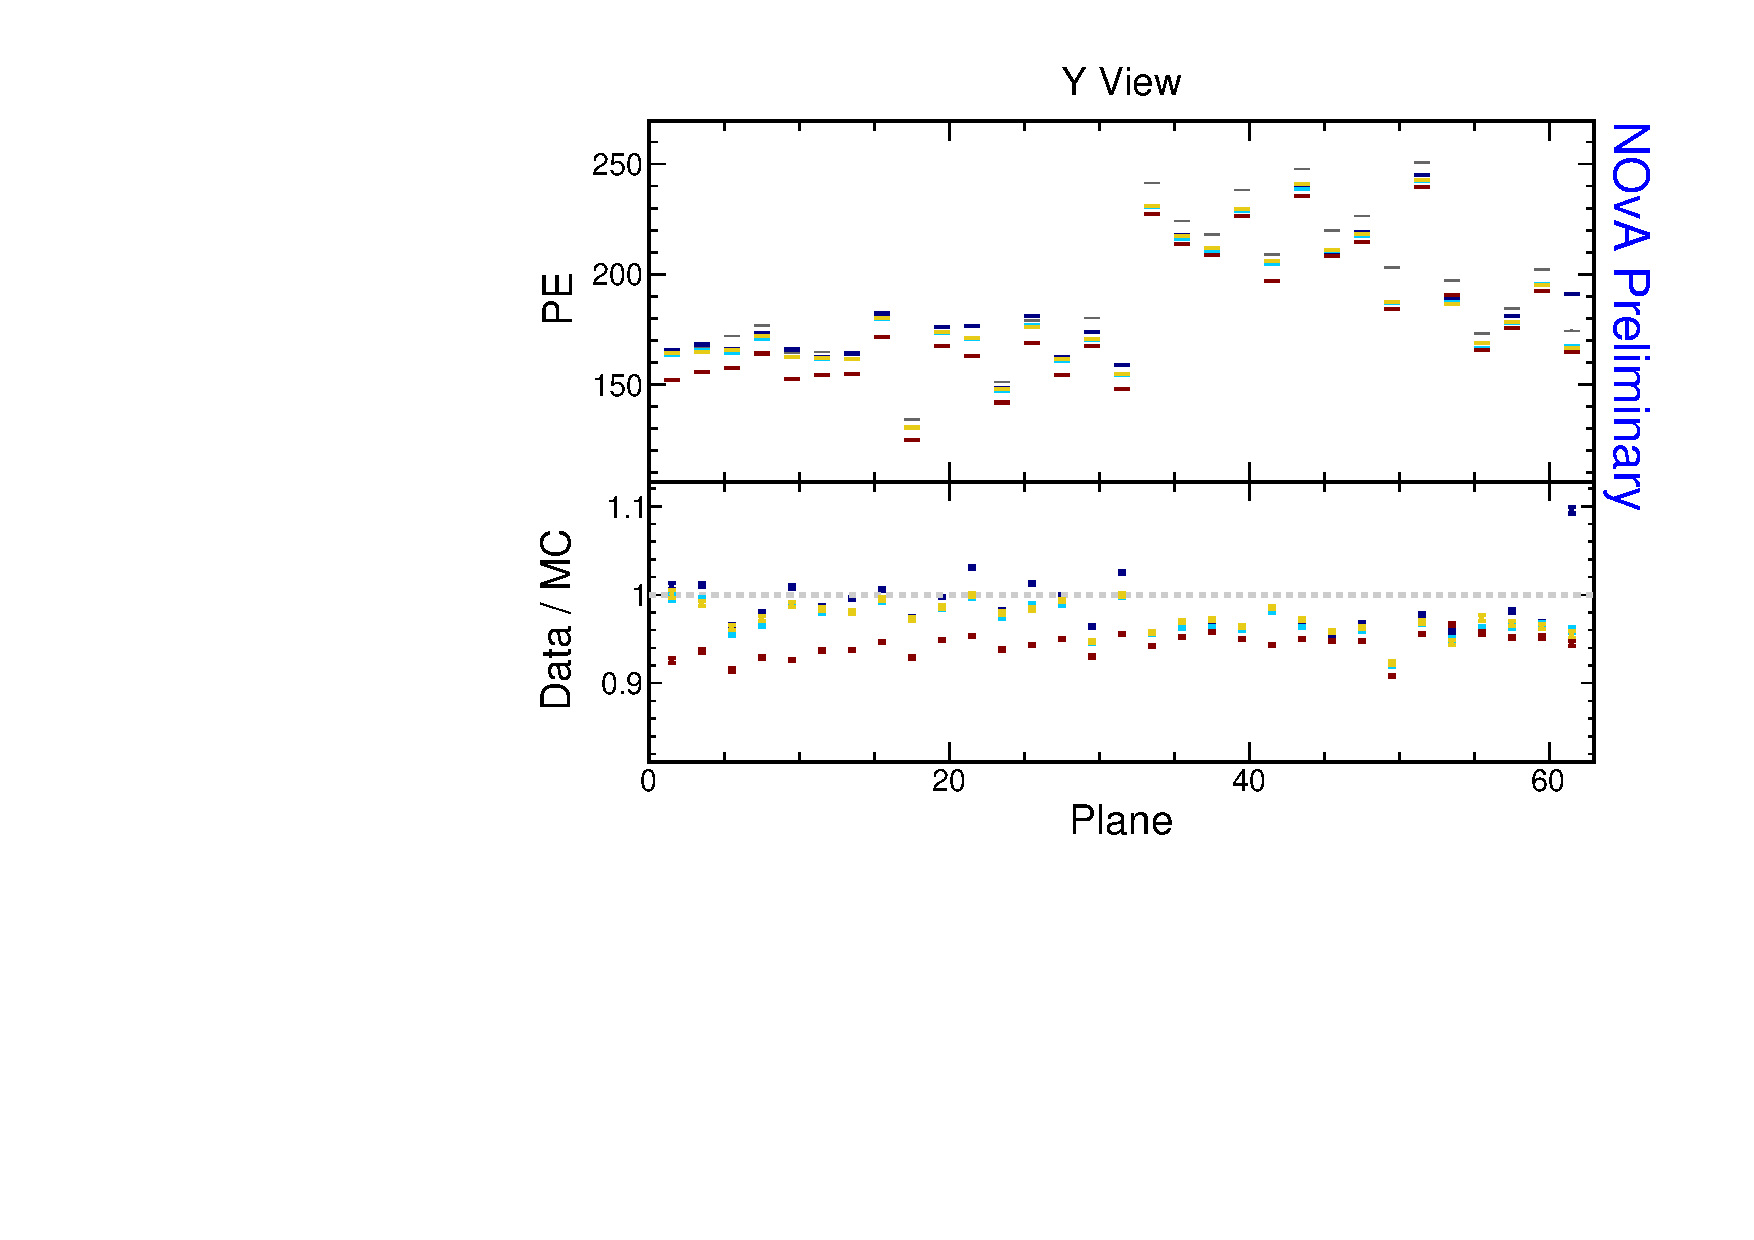
\includegraphics[width=\linewidth]{Plots/Calibana/pe_plane_y.pdf}
  \end{subfigure}
  \begin{subfigure}{0.495\textwidth}
    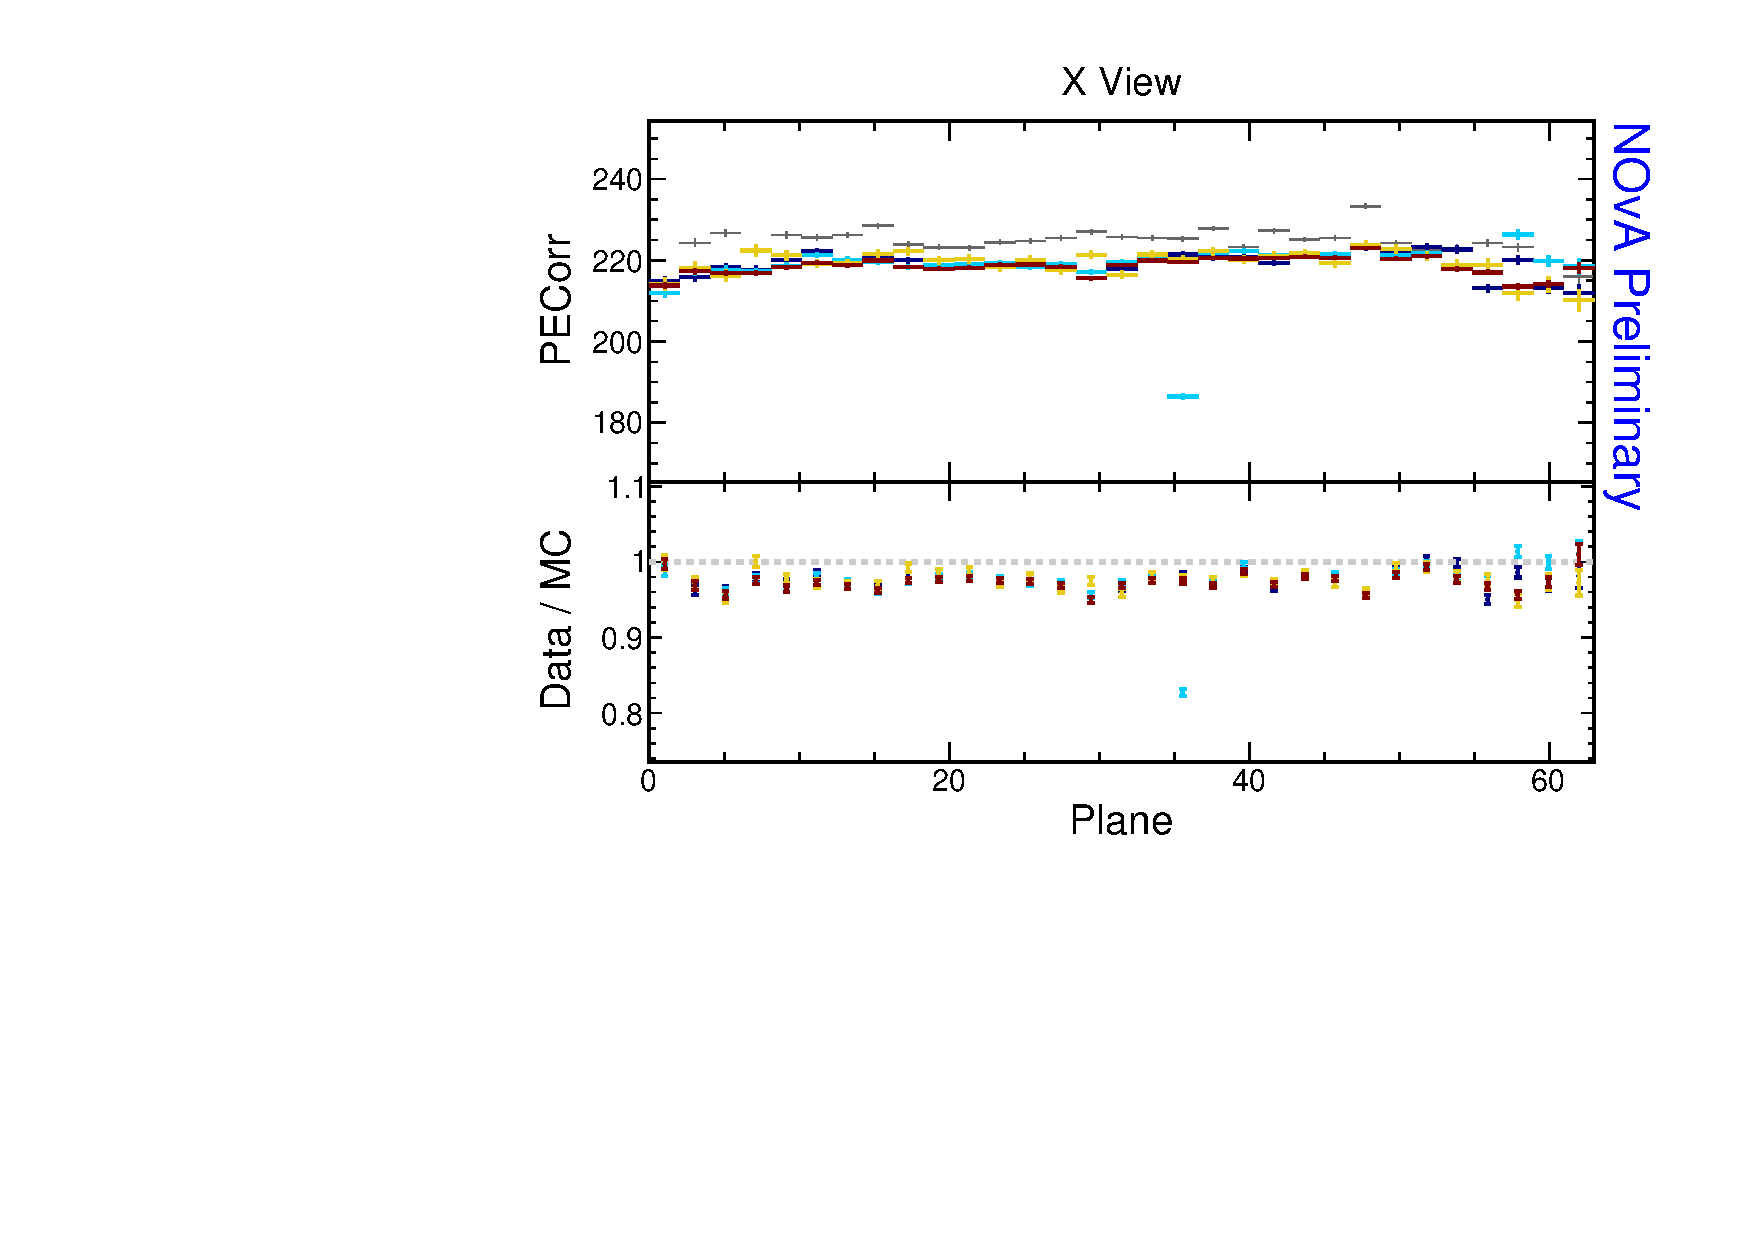
\includegraphics[width=\linewidth]{Plots/Calibana/pecorr_plane_x.pdf}
  \end{subfigure}
  \begin{subfigure}{0.495\textwidth}
    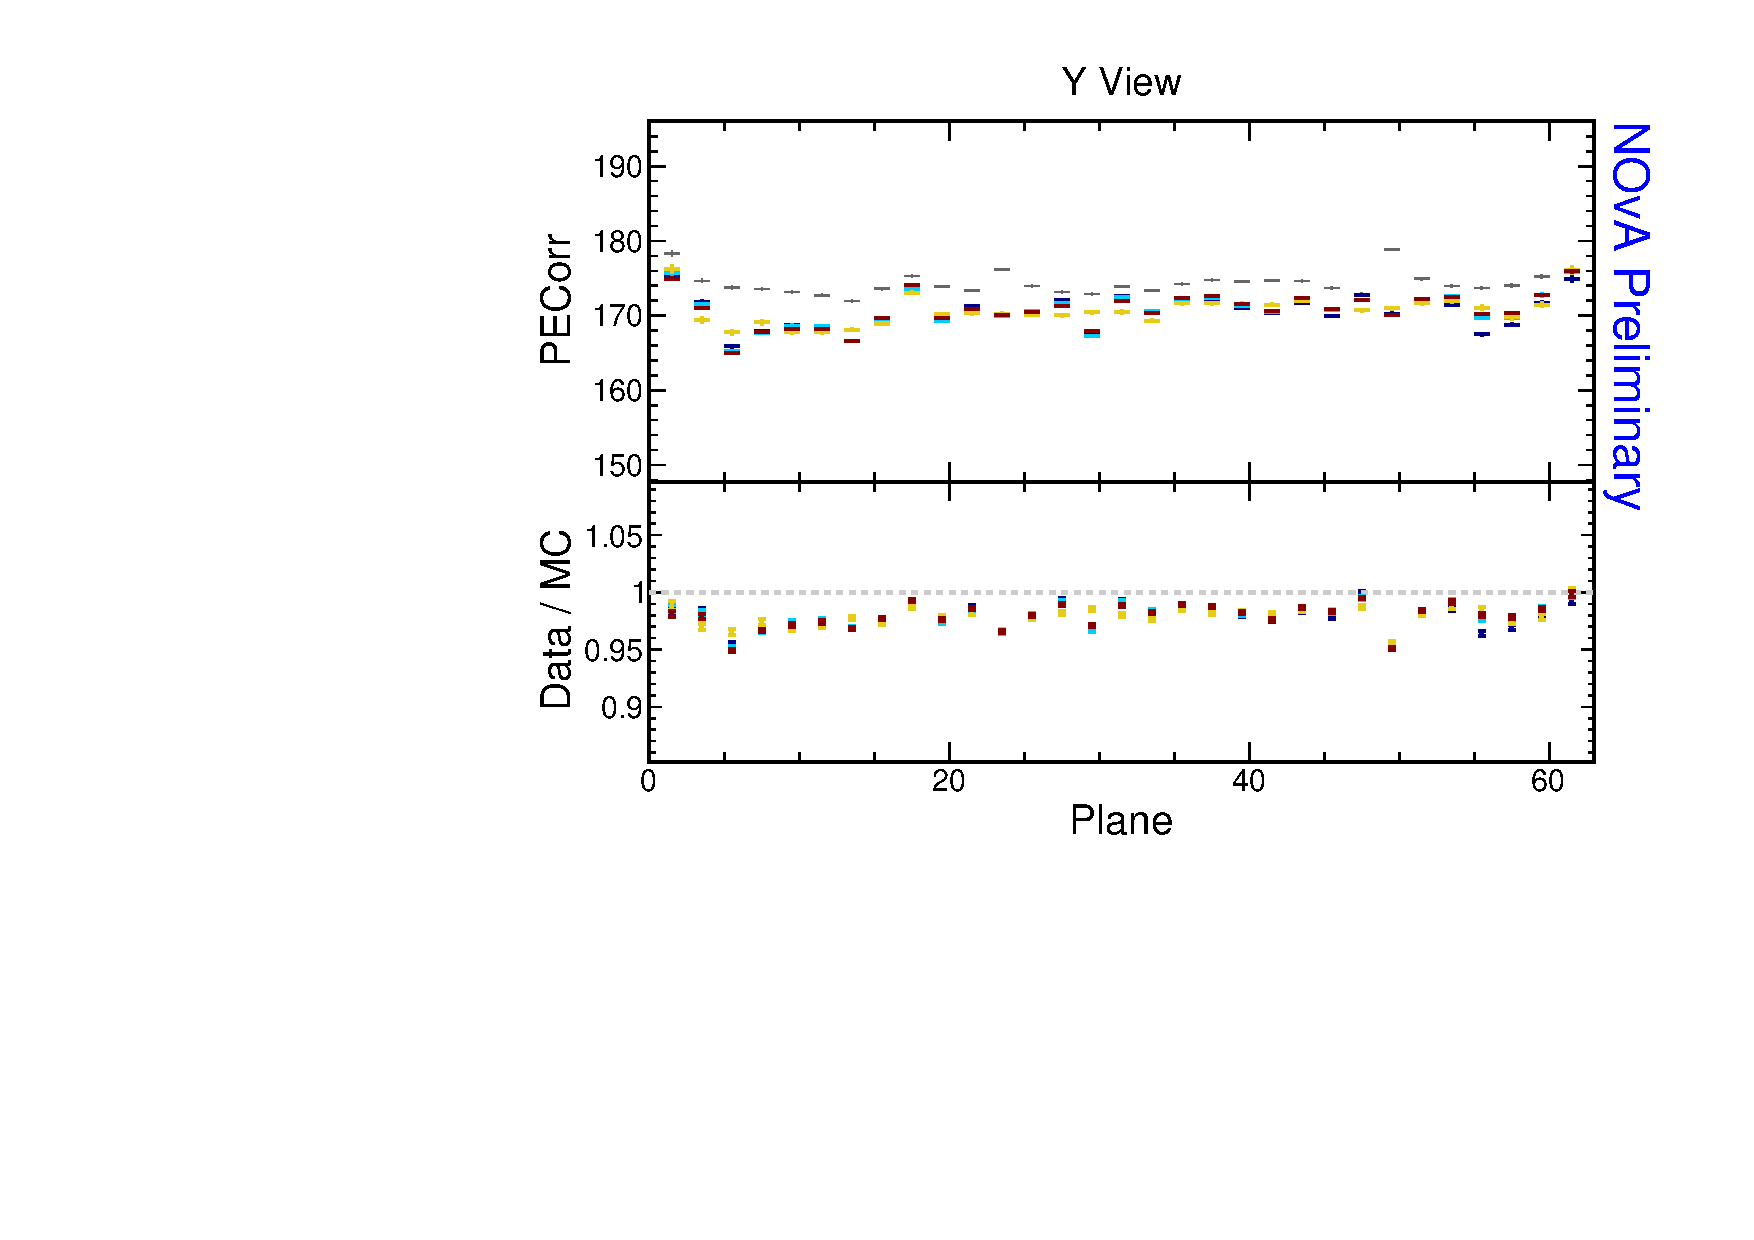
\includegraphics[width=\linewidth]{Plots/Calibana/pecorr_plane_y.pdf}
  \end{subfigure}
  \begin{subfigure}{0.495\textwidth}
    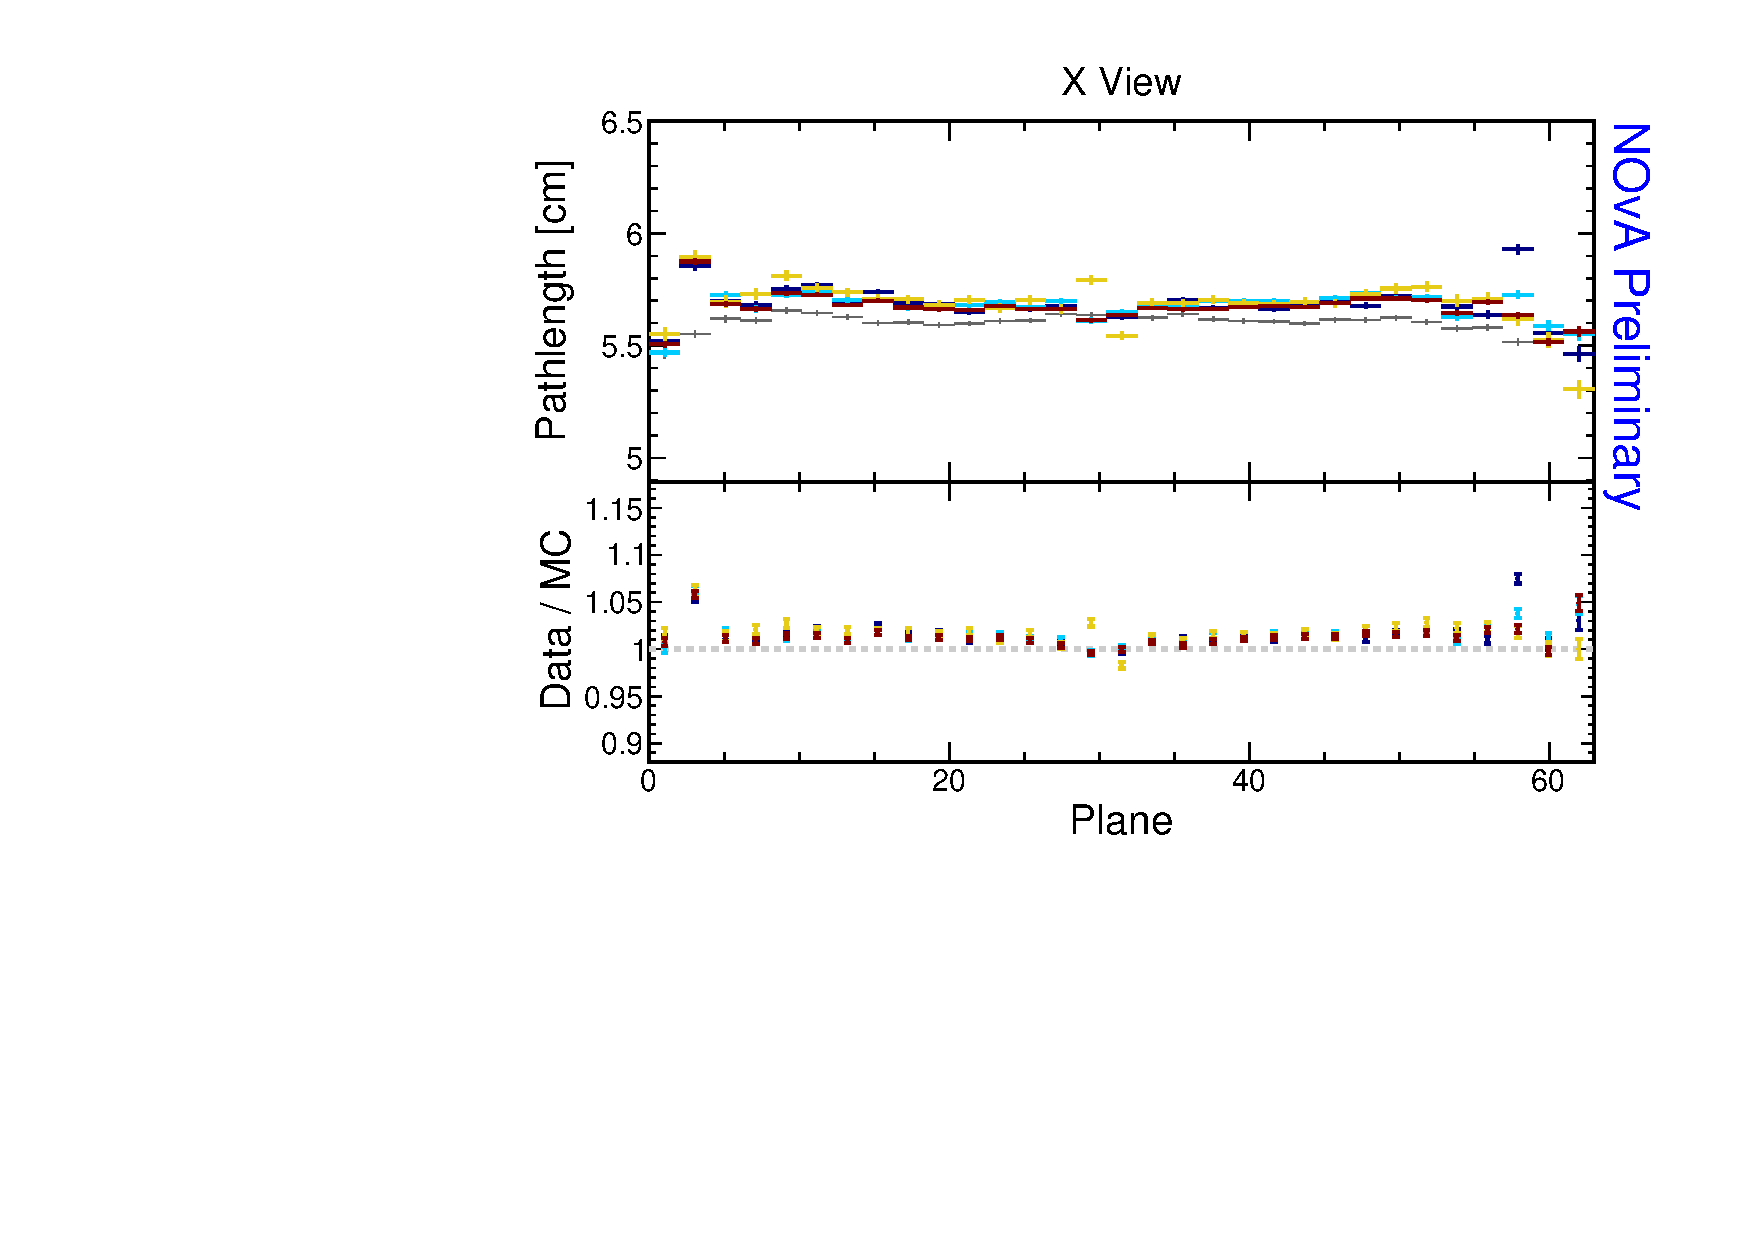
\includegraphics[width=\linewidth]{Plots/Calibana/cm_plane_x.pdf}
  \end{subfigure}
  \begin{subfigure}{0.495\textwidth}
    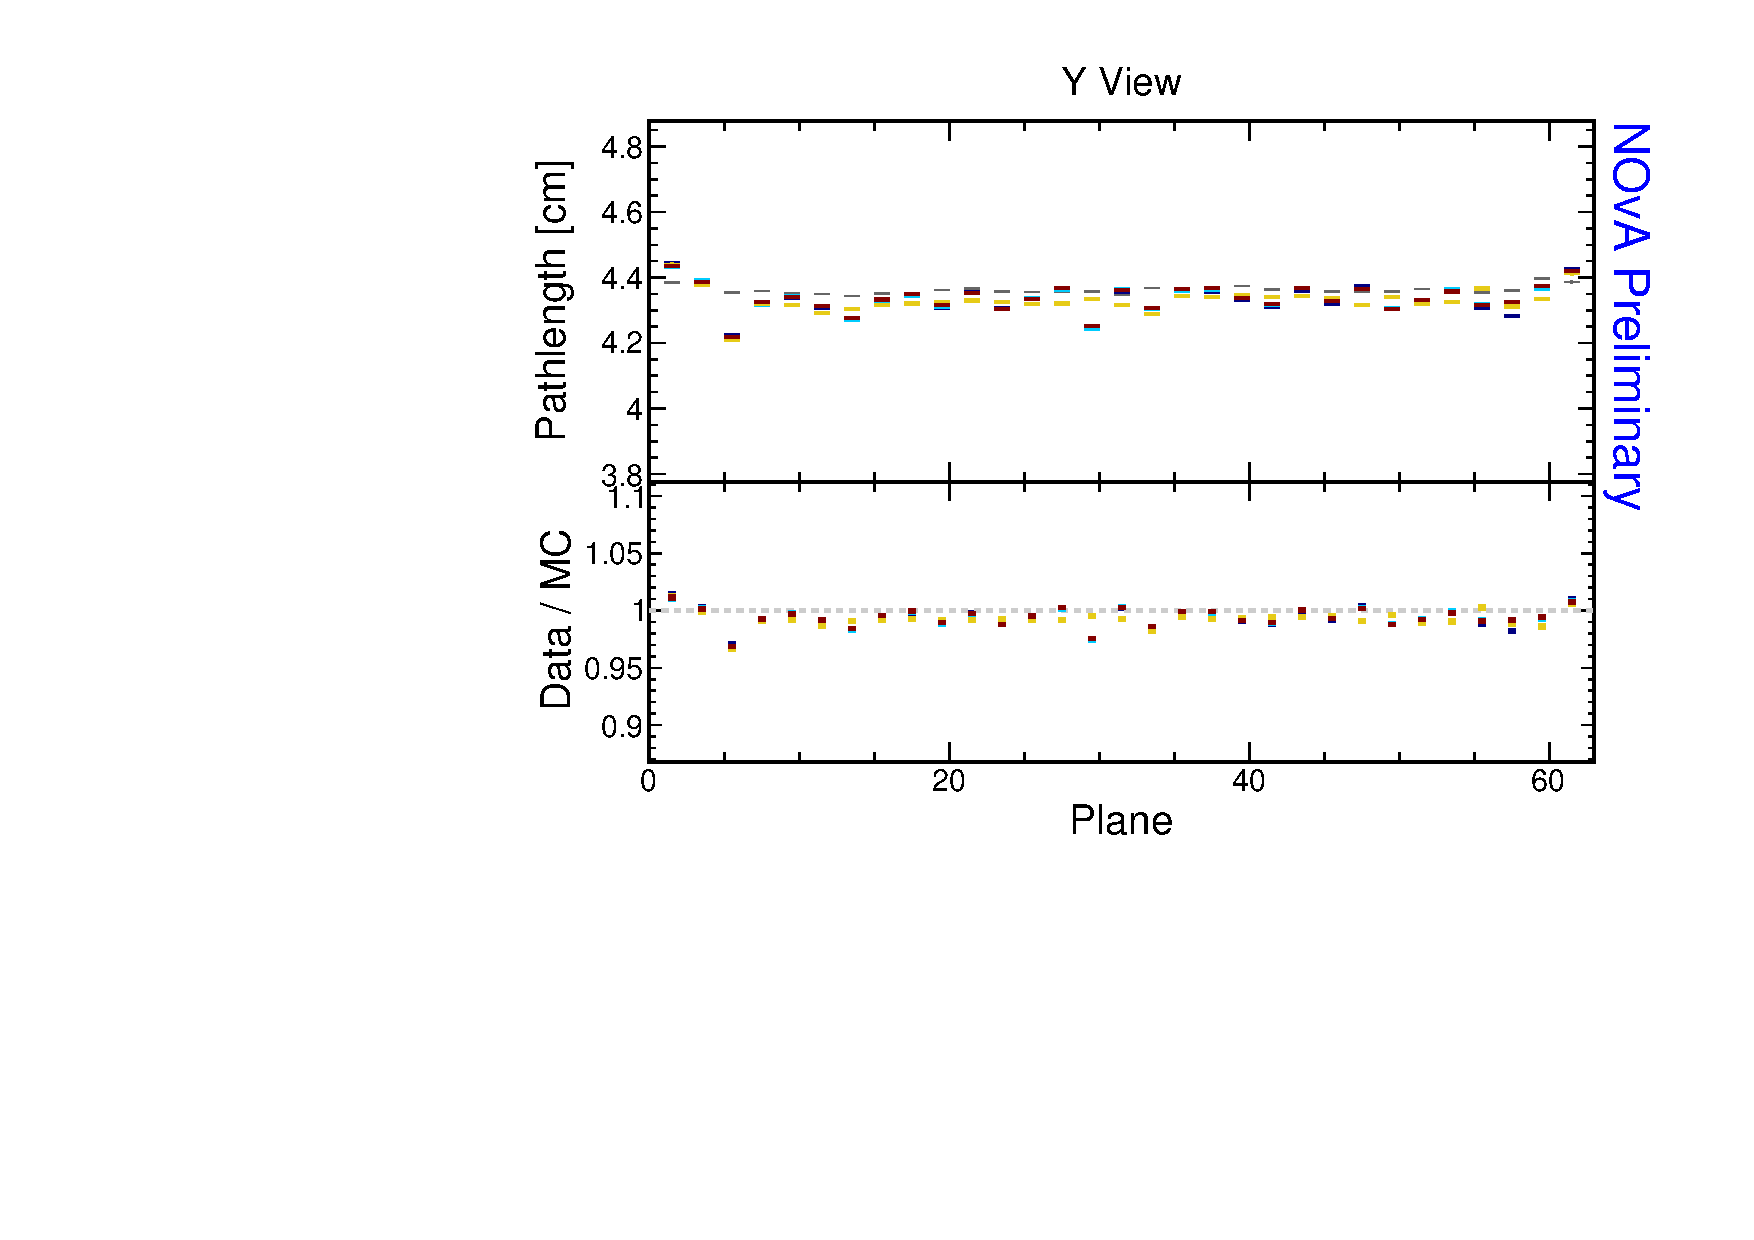
\includegraphics[width=\linewidth]{Plots/Calibana/cm_plane_y.pdf}
  \end{subfigure}
  \caption{Distributions of stopping muons within a 1-2 m track window from the end of their tracks across the planes of the detector.}
  %\label{fig:AbsCalibPlane2}
\end{figure}

\begin{figure}[!ht]
  \begin{subfigure}{\textwidth}
  \centering
    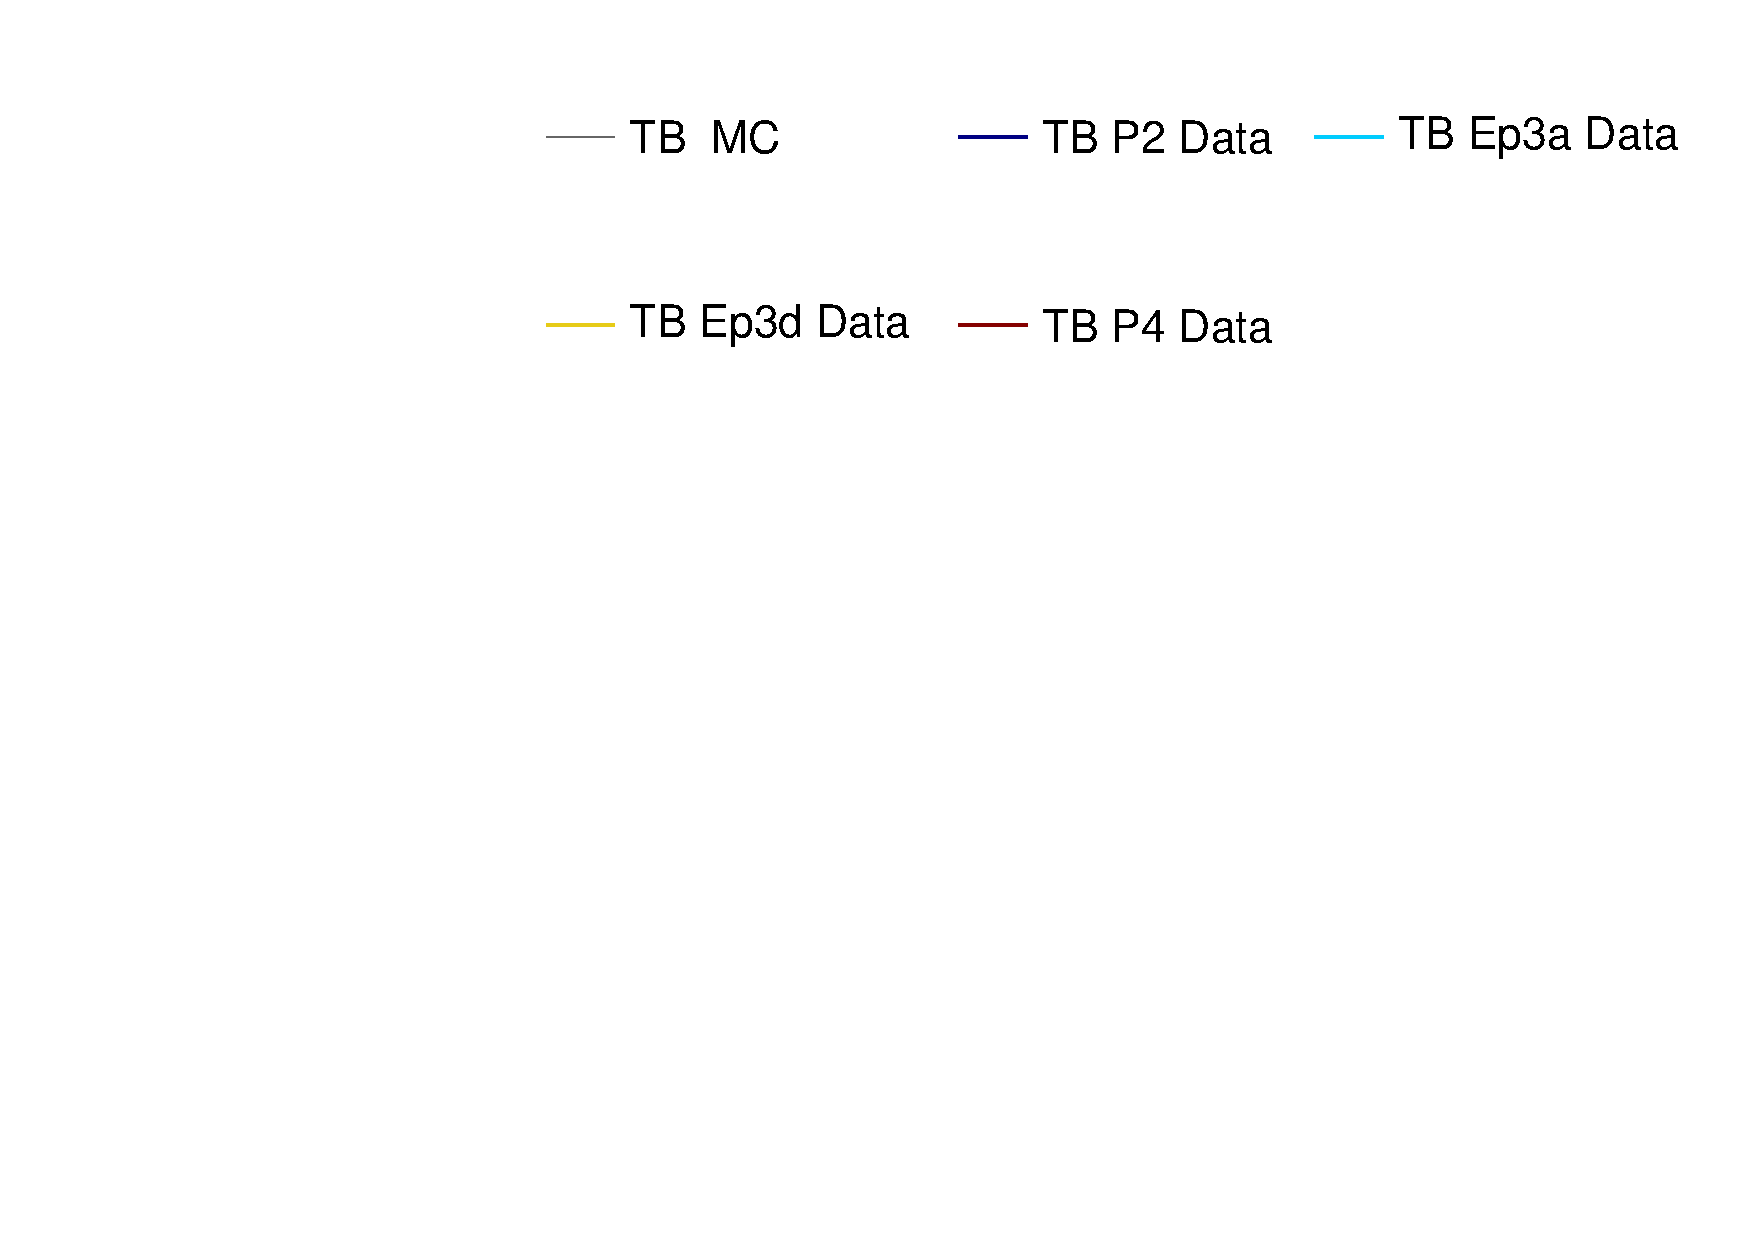
\includegraphics[height=0.2\linewidth]{Plots/Calibana/legend.pdf}
  \end{subfigure}
  \vspace*{2mm}

  \begin{subfigure}{0.495\textwidth}
    \includegraphics[width=\linewidth]{PlotsAngularDistribution/pecm_cosx_x.pdf}
  \end{subfigure}
  \begin{subfigure}{0.495\textwidth}
    \includegraphics[width=\linewidth]{PlotsAngularDistribution/pecm_cosx_y.pdf}
  \end{subfigure}
  \begin{subfigure}{0.495\textwidth}
    \includegraphics[width=\linewidth]{PlotsAngularDistribution/pecorrcm_cosx_x.pdf}
  \end{subfigure}
  \begin{subfigure}{0.495\textwidth}
    \includegraphics[width=\linewidth]{PlotsAngularDistribution/pecorrcm_cosx_y.pdf}
  \end{subfigure}
  \caption{Distributions of stopping muons within a 1-2 m track window from the end of their tracks across the cosine of the track angle from the X (horizontal) axis.}
  %\label{fig:AbsCalibCosX1}
\end{figure}

\begin{figure}[!ht]
  \begin{subfigure}{\textwidth}
  \centering
    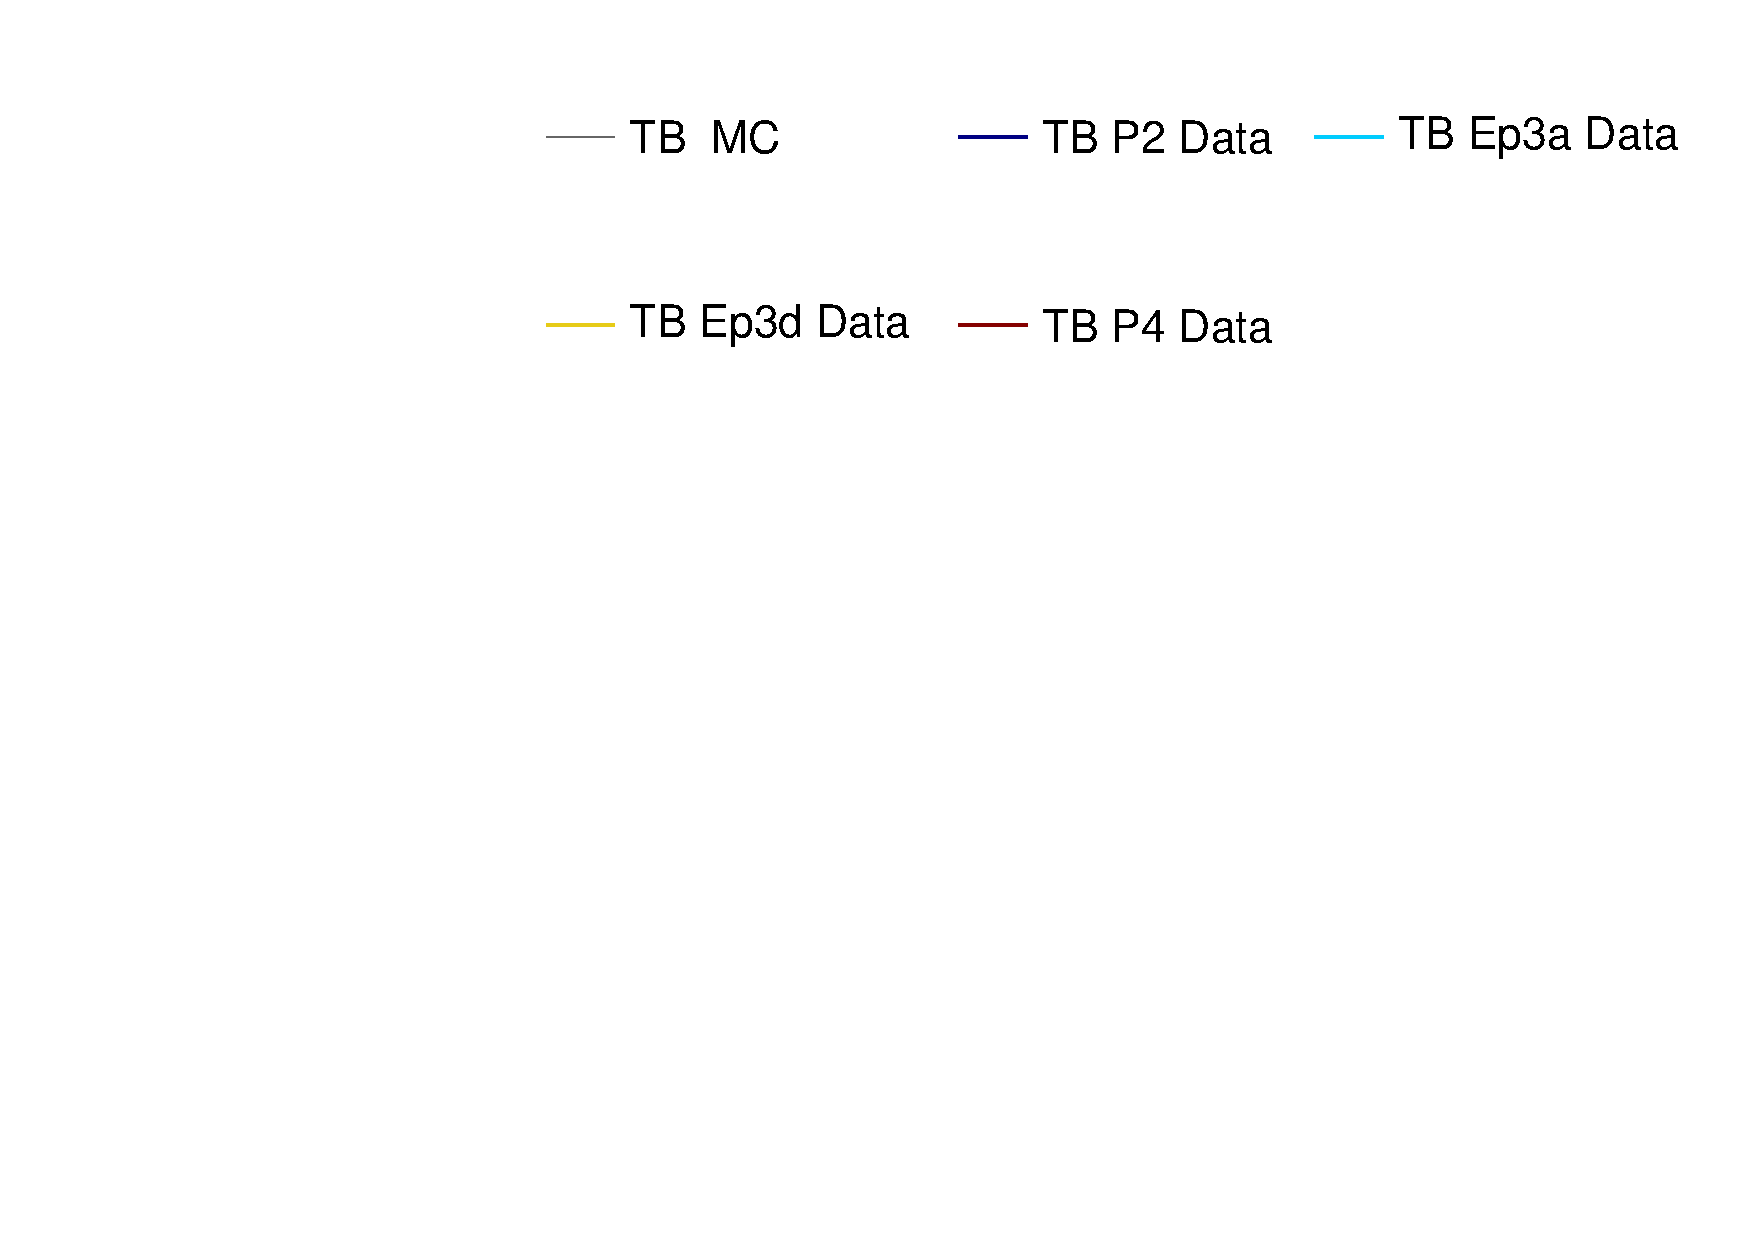
\includegraphics[height=0.2\linewidth]{Plots/Calibana/legend.pdf}
  \end{subfigure}
  \vspace*{2mm}

  \begin{subfigure}{0.495\textwidth}
    \includegraphics[width=\linewidth]{PlotsAngularDistribution/pe_cosx_x.pdf}
  \end{subfigure}
  \begin{subfigure}{0.495\textwidth}
    \includegraphics[width=\linewidth]{PlotsAngularDistribution/pe_cosx_y.pdf}
  \end{subfigure}
  \begin{subfigure}{0.495\textwidth}
    \includegraphics[width=\linewidth]{PlotsAngularDistribution/pecorr_cosx_x.pdf}
  \end{subfigure}
  \begin{subfigure}{0.495\textwidth}
    \includegraphics[width=\linewidth]{PlotsAngularDistribution/pecorr_cosx_y.pdf}
  \end{subfigure}
  \begin{subfigure}{0.495\textwidth}
    \includegraphics[width=\linewidth]{PlotsAngularDistribution/cm_cosx_x.pdf}
  \end{subfigure}
  \begin{subfigure}{0.495\textwidth}
    \includegraphics[width=\linewidth]{PlotsAngularDistribution/cm_cosx_y.pdf}
  \end{subfigure}
  \caption{Distributions of stopping muons within a 1-2 m track window from the end of their tracks across the cosine of the track angle from the X (horizontal) axis.}
  %\label{fig:AbsCalibCosX2}
\end{figure}

\begin{figure}[!ht]
  \begin{subfigure}{\textwidth}
  \centering
    \includegraphics[height=0.2\linewidth]{Plots/Calibana/legend.pdf}
  \end{subfigure}
  \vspace*{2mm}
  
  \begin{subfigure}{0.495\textwidth}
    \includegraphics[width=\linewidth]{PlotsAngularDistribution/pecm_cosy_x.pdf}
  \end{subfigure}
  \begin{subfigure}{0.495\textwidth}
    \includegraphics[width=\linewidth]{PlotsAngularDistribution/pecm_cosy_y.pdf}
  \end{subfigure}
  \begin{subfigure}{0.495\textwidth}
    \includegraphics[width=\linewidth]{PlotsAngularDistribution/pecorrcm_cosy_x.pdf}
  \end{subfigure}
  \begin{subfigure}{0.495\textwidth}
    \includegraphics[width=\linewidth]{PlotsAngularDistribution/pecorrcm_cosy_y.pdf}
  \end{subfigure}
  \caption{Distributions of stopping muons within a 1-2 m track window from the end of their tracks across the cosine of the track angle from the Y (vertical) axis.}
  %\label{fig:AbsCalibCosY1}
\end{figure}

\begin{figure}[!ht]
  \begin{subfigure}{\textwidth}
  \centering
    \includegraphics[height=0.2\linewidth]{Plots/Calibana/legend.pdf}
  \end{subfigure}
  \vspace*{2mm}

  \begin{subfigure}{0.495\textwidth}
    \includegraphics[width=\linewidth]{PlotsAngularDistribution/pe_cosy_x.pdf}
  \end{subfigure}
  \begin{subfigure}{0.495\textwidth}
    \includegraphics[width=\linewidth]{PlotsAngularDistribution/pe_cosy_y.pdf}
  \end{subfigure}
  \begin{subfigure}{0.495\textwidth}
    \includegraphics[width=\linewidth]{PlotsAngularDistribution/pecorr_cosy_x.pdf}
  \end{subfigure}
  \begin{subfigure}{0.495\textwidth}
    \includegraphics[width=\linewidth]{PlotsAngularDistribution/pecorr_cosy_y.pdf}
  \end{subfigure}
  \begin{subfigure}{0.495\textwidth}
    \includegraphics[width=\linewidth]{PlotsAngularDistribution/cm_cosy_x.pdf}
  \end{subfigure}
  \begin{subfigure}{0.495\textwidth}
    \includegraphics[width=\linewidth]{PlotsAngularDistribution/cm_cosy_y.pdf}
  \end{subfigure}
  \caption{Distributions of stopping muons within a 1-2 m track window from the end of their tracks across the cosine of the track angle from the Y (vertical) axis.}
  %\label{fig:AbsCalibCosY2}
\end{figure}

\begin{figure}[!ht]
  \begin{subfigure}{\textwidth}
  \centering
    \includegraphics[height=0.2\linewidth]{Plots/Calibana/legend.pdf}
  \end{subfigure}
  \vspace*{2mm}
  
  \begin{subfigure}{0.495\textwidth}
    \includegraphics[width=\linewidth]{PlotsAngularDistribution/pecm_cosz_x.pdf}
  \end{subfigure}
  \begin{subfigure}{0.495\textwidth}
    \includegraphics[width=\linewidth]{PlotsAngularDistribution/pecm_cosz_y.pdf}
  \end{subfigure}
  \begin{subfigure}{0.495\textwidth}
    \includegraphics[width=\linewidth]{PlotsAngularDistribution/pecorrcm_cosz_x.pdf}
  \end{subfigure}
  \begin{subfigure}{0.495\textwidth}
    \includegraphics[width=\linewidth]{PlotsAngularDistribution/pecorrcm_cosz_y.pdf}
  \end{subfigure}
  \caption{Distributions of stopping muons within a 1-2 m track window from the end of their tracks across the cosine of the track angle from the Z (beam) axis.}
  %\label{fig:AbsCalibCosZ1}
\end{figure}

\begin{figure}[!ht]
  \begin{subfigure}{\textwidth}
    \centering
    \includegraphics[height=0.2\linewidth]{Plots/Calibana/legend.pdf}
  \end{subfigure}
  \vspace*{2mm}
  
  \begin{subfigure}{0.5\textwidth}
    \includegraphics[width=\linewidth]{PlotsAngularDistribution/pe_cosz_x.pdf}
  \end{subfigure}
  \begin{subfigure}{0.495\textwidth}
    \includegraphics[width=\linewidth]{PlotsAngularDistribution/pe_cosz_y.pdf}
  \end{subfigure}
  \begin{subfigure}{0.495\textwidth}
    \includegraphics[width=\linewidth]{PlotsAngularDistribution/pecorr_cosz_x.pdf}
  \end{subfigure}
  \begin{subfigure}{0.495\textwidth}
    \includegraphics[width=\linewidth]{PlotsAngularDistribution/pecorr_cosz_y.pdf}
  \end{subfigure}
  \begin{subfigure}{0.495\textwidth}
    \includegraphics[width=\linewidth]{PlotsAngularDistribution/cm_cosz_x.pdf}
  \end{subfigure}
  \begin{subfigure}{0.495\textwidth}
    \includegraphics[width=\linewidth]{PlotsAngularDistribution/cm_cosz_y.pdf}
  \end{subfigure}
  \caption{Distributions of stopping muons within a 1-2 m track window from the end of their tracks across the cosine of the track angle from the Z (beam) axis.}
  %\label{fig:AbsCalibCosZ2}
\end{figure}

%\subsection{Drift in TB data}

\begin{figure}[!ht]
  \begin{subfigure}{\textwidth}
    \centering
    \includegraphics[height=0.2\linewidth]{Plots/Calibana/legend.pdf}
  \end{subfigure}
  \vspace*{2mm}
  
  \begin{subfigure}{0.495\textwidth}
    \includegraphics[width=\linewidth]{Plots/Calibana/pecm_time_x.pdf}
  \end{subfigure}
  \begin{subfigure}{0.495\textwidth}
    \includegraphics[width=\linewidth]{Plots/Calibana/pecm_time_y.pdf}
  \end{subfigure}
  \begin{subfigure}{0.495\textwidth}
    \includegraphics[width=\linewidth]{Plots/Calibana/pecorrcm_time_x.pdf}
  \end{subfigure}
  \begin{subfigure}{0.495\textwidth}
    \includegraphics[width=\linewidth]{Plots/Calibana/pecorrcm_time_y.pdf}
  \end{subfigure}
    \begin{subfigure}{0.495\textwidth}
    \includegraphics[width=\linewidth]{Plots/Calibana/recomevcm_time_x.pdf}
  \end{subfigure}
  \begin{subfigure}{0.495\textwidth}
    \includegraphics[width=\linewidth]{Plots/Calibana/recomevcm_time_y.pdf}
  \end{subfigure}
  \caption{Distributions of stopping muons within a 1-2 m track window from the end of their tracks across the event UNIX time.}
  %\label{fig:AbsCalibDrift1}
\end{figure}

\begin{figure}[!ht]
  \begin{subfigure}{\textwidth}
    \centering
    \includegraphics[height=0.2\linewidth]{Plots/Calibana/legend.pdf}
  \end{subfigure}
  \vspace*{2mm}
  
  \begin{subfigure}{0.495\textwidth}
    \includegraphics[width=\linewidth]{Plots/Calibana/pe_time_x.pdf}
  \end{subfigure}
  \begin{subfigure}{0.495\textwidth}
    \includegraphics[width=\linewidth]{Plots/Calibana/pe_time_y.pdf}
  \end{subfigure}
  \begin{subfigure}{0.495\textwidth}
    \includegraphics[width=\linewidth]{Plots/Calibana/pecorr_time_x.pdf}
  \end{subfigure}
  \begin{subfigure}{0.495\textwidth}
    \includegraphics[width=\linewidth]{Plots/Calibana/pecorr_time_y.pdf}
  \end{subfigure}
  \begin{subfigure}{0.495\textwidth}
    \includegraphics[width=\linewidth]{Plots/Calibana/cm_time_x.pdf}
  \end{subfigure}
  \begin{subfigure}{0.495\textwidth}
    \includegraphics[width=\linewidth]{Plots/Calibana/cm_time_y.pdf}
  \end{subfigure}
  \caption{Distributions of stopping muons within a 1-2 m track window from the end of their tracks across the event UNIX time.}
  %\label{fig:AbsCalibDrift2}
\end{figure}


\begin{figure}[ht!]
  \begin{subfigure}{\textwidth}
	\centering
   	\includegraphics[height=0.2\linewidth]{Plots/Calibana/legend.pdf}
  \end{subfigure}
  \vspace*{2mm}
  
  \begin{subfigure}{0.495\textwidth}
    \includegraphics[width=\linewidth]{Plots/Calibana/nhits_w_x.pdf}
  \end{subfigure}
  \begin{subfigure}{0.495\textwidth}
    \includegraphics[width=\linewidth]{Plots/Calibana/nhits_w_y.pdf}
  \end{subfigure}
  \begin{subfigure}{0.495\textwidth}
    \includegraphics[width=\linewidth]{Plots/Calibana/nhits_cell_x.pdf}
  \end{subfigure}
  \begin{subfigure}{0.495\textwidth}
    \includegraphics[width=\linewidth]{Plots/Calibana/nhits_cell_y.pdf}
  \end{subfigure}
  \begin{subfigure}{0.495\textwidth}
    \includegraphics[width=\linewidth]{Plots/Calibana/nhits_plane_x.pdf}
  \end{subfigure}
  \begin{subfigure}{0.495\textwidth}
    \includegraphics[width=\linewidth]{Plots/Calibana/nhits_plane_y.pdf}
  \end{subfigure}
    \caption{Distributions of stopping muons within a 1-2 m track window from the end of their tracks.}
  %\label{fig:AbsCalibNHitsWCellPlane}
\end{figure}
